% Options for packages loaded elsewhere
\PassOptionsToPackage{unicode}{hyperref}
\PassOptionsToPackage{hyphens}{url}
\PassOptionsToPackage{dvipsnames,svgnames,x11names}{xcolor}
%
\documentclass[
  letterpaper,
  DIV=11,
  numbers=noendperiod]{scrreprt}

\usepackage{amsmath,amssymb}
\usepackage{lmodern}
\usepackage{iftex}
\ifPDFTeX
  \usepackage[T1]{fontenc}
  \usepackage[utf8]{inputenc}
  \usepackage{textcomp} % provide euro and other symbols
\else % if luatex or xetex
  \usepackage{unicode-math}
  \defaultfontfeatures{Scale=MatchLowercase}
  \defaultfontfeatures[\rmfamily]{Ligatures=TeX,Scale=1}
\fi
% Use upquote if available, for straight quotes in verbatim environments
\IfFileExists{upquote.sty}{\usepackage{upquote}}{}
\IfFileExists{microtype.sty}{% use microtype if available
  \usepackage[]{microtype}
  \UseMicrotypeSet[protrusion]{basicmath} % disable protrusion for tt fonts
}{}
\makeatletter
\@ifundefined{KOMAClassName}{% if non-KOMA class
  \IfFileExists{parskip.sty}{%
    \usepackage{parskip}
  }{% else
    \setlength{\parindent}{0pt}
    \setlength{\parskip}{6pt plus 2pt minus 1pt}}
}{% if KOMA class
  \KOMAoptions{parskip=half}}
\makeatother
\usepackage{xcolor}
\setlength{\emergencystretch}{3em} % prevent overfull lines
\setcounter{secnumdepth}{5}
% Make \paragraph and \subparagraph free-standing
\ifx\paragraph\undefined\else
  \let\oldparagraph\paragraph
  \renewcommand{\paragraph}[1]{\oldparagraph{#1}\mbox{}}
\fi
\ifx\subparagraph\undefined\else
  \let\oldsubparagraph\subparagraph
  \renewcommand{\subparagraph}[1]{\oldsubparagraph{#1}\mbox{}}
\fi

\usepackage{color}
\usepackage{fancyvrb}
\newcommand{\VerbBar}{|}
\newcommand{\VERB}{\Verb[commandchars=\\\{\}]}
\DefineVerbatimEnvironment{Highlighting}{Verbatim}{commandchars=\\\{\}}
% Add ',fontsize=\small' for more characters per line
\usepackage{framed}
\definecolor{shadecolor}{RGB}{241,243,245}
\newenvironment{Shaded}{\begin{snugshade}}{\end{snugshade}}
\newcommand{\AlertTok}[1]{\textcolor[rgb]{0.68,0.00,0.00}{#1}}
\newcommand{\AnnotationTok}[1]{\textcolor[rgb]{0.37,0.37,0.37}{#1}}
\newcommand{\AttributeTok}[1]{\textcolor[rgb]{0.40,0.45,0.13}{#1}}
\newcommand{\BaseNTok}[1]{\textcolor[rgb]{0.68,0.00,0.00}{#1}}
\newcommand{\BuiltInTok}[1]{\textcolor[rgb]{0.00,0.23,0.31}{#1}}
\newcommand{\CharTok}[1]{\textcolor[rgb]{0.13,0.47,0.30}{#1}}
\newcommand{\CommentTok}[1]{\textcolor[rgb]{0.37,0.37,0.37}{#1}}
\newcommand{\CommentVarTok}[1]{\textcolor[rgb]{0.37,0.37,0.37}{\textit{#1}}}
\newcommand{\ConstantTok}[1]{\textcolor[rgb]{0.56,0.35,0.01}{#1}}
\newcommand{\ControlFlowTok}[1]{\textcolor[rgb]{0.00,0.23,0.31}{#1}}
\newcommand{\DataTypeTok}[1]{\textcolor[rgb]{0.68,0.00,0.00}{#1}}
\newcommand{\DecValTok}[1]{\textcolor[rgb]{0.68,0.00,0.00}{#1}}
\newcommand{\DocumentationTok}[1]{\textcolor[rgb]{0.37,0.37,0.37}{\textit{#1}}}
\newcommand{\ErrorTok}[1]{\textcolor[rgb]{0.68,0.00,0.00}{#1}}
\newcommand{\ExtensionTok}[1]{\textcolor[rgb]{0.00,0.23,0.31}{#1}}
\newcommand{\FloatTok}[1]{\textcolor[rgb]{0.68,0.00,0.00}{#1}}
\newcommand{\FunctionTok}[1]{\textcolor[rgb]{0.28,0.35,0.67}{#1}}
\newcommand{\ImportTok}[1]{\textcolor[rgb]{0.00,0.46,0.62}{#1}}
\newcommand{\InformationTok}[1]{\textcolor[rgb]{0.37,0.37,0.37}{#1}}
\newcommand{\KeywordTok}[1]{\textcolor[rgb]{0.00,0.23,0.31}{#1}}
\newcommand{\NormalTok}[1]{\textcolor[rgb]{0.00,0.23,0.31}{#1}}
\newcommand{\OperatorTok}[1]{\textcolor[rgb]{0.37,0.37,0.37}{#1}}
\newcommand{\OtherTok}[1]{\textcolor[rgb]{0.00,0.23,0.31}{#1}}
\newcommand{\PreprocessorTok}[1]{\textcolor[rgb]{0.68,0.00,0.00}{#1}}
\newcommand{\RegionMarkerTok}[1]{\textcolor[rgb]{0.00,0.23,0.31}{#1}}
\newcommand{\SpecialCharTok}[1]{\textcolor[rgb]{0.37,0.37,0.37}{#1}}
\newcommand{\SpecialStringTok}[1]{\textcolor[rgb]{0.13,0.47,0.30}{#1}}
\newcommand{\StringTok}[1]{\textcolor[rgb]{0.13,0.47,0.30}{#1}}
\newcommand{\VariableTok}[1]{\textcolor[rgb]{0.07,0.07,0.07}{#1}}
\newcommand{\VerbatimStringTok}[1]{\textcolor[rgb]{0.13,0.47,0.30}{#1}}
\newcommand{\WarningTok}[1]{\textcolor[rgb]{0.37,0.37,0.37}{\textit{#1}}}

\providecommand{\tightlist}{%
  \setlength{\itemsep}{0pt}\setlength{\parskip}{0pt}}\usepackage{longtable,booktabs,array}
\usepackage{calc} % for calculating minipage widths
% Correct order of tables after \paragraph or \subparagraph
\usepackage{etoolbox}
\makeatletter
\patchcmd\longtable{\par}{\if@noskipsec\mbox{}\fi\par}{}{}
\makeatother
% Allow footnotes in longtable head/foot
\IfFileExists{footnotehyper.sty}{\usepackage{footnotehyper}}{\usepackage{footnote}}
\makesavenoteenv{longtable}
\usepackage{graphicx}
\makeatletter
\def\maxwidth{\ifdim\Gin@nat@width>\linewidth\linewidth\else\Gin@nat@width\fi}
\def\maxheight{\ifdim\Gin@nat@height>\textheight\textheight\else\Gin@nat@height\fi}
\makeatother
% Scale images if necessary, so that they will not overflow the page
% margins by default, and it is still possible to overwrite the defaults
% using explicit options in \includegraphics[width, height, ...]{}
\setkeys{Gin}{width=\maxwidth,height=\maxheight,keepaspectratio}
% Set default figure placement to htbp
\makeatletter
\def\fps@figure{htbp}
\makeatother
\newlength{\cslhangindent}
\setlength{\cslhangindent}{1.5em}
\newlength{\csllabelwidth}
\setlength{\csllabelwidth}{3em}
\newlength{\cslentryspacingunit} % times entry-spacing
\setlength{\cslentryspacingunit}{\parskip}
\newenvironment{CSLReferences}[2] % #1 hanging-ident, #2 entry spacing
 {% don't indent paragraphs
  \setlength{\parindent}{0pt}
  % turn on hanging indent if param 1 is 1
  \ifodd #1
  \let\oldpar\par
  \def\par{\hangindent=\cslhangindent\oldpar}
  \fi
  % set entry spacing
  \setlength{\parskip}{#2\cslentryspacingunit}
 }%
 {}
\usepackage{calc}
\newcommand{\CSLBlock}[1]{#1\hfill\break}
\newcommand{\CSLLeftMargin}[1]{\parbox[t]{\csllabelwidth}{#1}}
\newcommand{\CSLRightInline}[1]{\parbox[t]{\linewidth - \csllabelwidth}{#1}\break}
\newcommand{\CSLIndent}[1]{\hspace{\cslhangindent}#1}

\usepackage{booktabs}
\usepackage{longtable}
\usepackage{array}
\usepackage{multirow}
\usepackage{wrapfig}
\usepackage{float}
\usepackage{colortbl}
\usepackage{pdflscape}
\usepackage{tabu}
\usepackage{threeparttable}
\usepackage{threeparttablex}
\usepackage[normalem]{ulem}
\usepackage{makecell}
\usepackage{xcolor}
\KOMAoption{captions}{tableheading}
\makeatletter
\makeatother
\makeatletter
\@ifpackageloaded{bookmark}{}{\usepackage{bookmark}}
\makeatother
\makeatletter
\@ifpackageloaded{caption}{}{\usepackage{caption}}
\AtBeginDocument{%
\ifdefined\contentsname
  \renewcommand*\contentsname{Table of contents}
\else
  \newcommand\contentsname{Table of contents}
\fi
\ifdefined\listfigurename
  \renewcommand*\listfigurename{List of Figures}
\else
  \newcommand\listfigurename{List of Figures}
\fi
\ifdefined\listtablename
  \renewcommand*\listtablename{List of Tables}
\else
  \newcommand\listtablename{List of Tables}
\fi
\ifdefined\figurename
  \renewcommand*\figurename{Figure}
\else
  \newcommand\figurename{Figure}
\fi
\ifdefined\tablename
  \renewcommand*\tablename{Table}
\else
  \newcommand\tablename{Table}
\fi
}
\@ifpackageloaded{float}{}{\usepackage{float}}
\floatstyle{ruled}
\@ifundefined{c@chapter}{\newfloat{codelisting}{h}{lop}}{\newfloat{codelisting}{h}{lop}[chapter]}
\floatname{codelisting}{Listing}
\newcommand*\listoflistings{\listof{codelisting}{List of Listings}}
\makeatother
\makeatletter
\@ifpackageloaded{caption}{}{\usepackage{caption}}
\@ifpackageloaded{subcaption}{}{\usepackage{subcaption}}
\makeatother
\makeatletter
\@ifpackageloaded{tcolorbox}{}{\usepackage[many]{tcolorbox}}
\makeatother
\makeatletter
\@ifundefined{shadecolor}{\definecolor{shadecolor}{rgb}{.97, .97, .97}}
\makeatother
\makeatletter
\makeatother
\ifLuaTeX
  \usepackage{selnolig}  % disable illegal ligatures
\fi
\IfFileExists{bookmark.sty}{\usepackage{bookmark}}{\usepackage{hyperref}}
\IfFileExists{xurl.sty}{\usepackage{xurl}}{} % add URL line breaks if available
\urlstyle{same} % disable monospaced font for URLs
\hypersetup{
  pdftitle={Metagad experiment example},
  pdfauthor={MetaDag Team},
  colorlinks=true,
  linkcolor={blue},
  filecolor={Maroon},
  citecolor={Blue},
  urlcolor={Blue},
  pdfcreator={LaTeX via pandoc}}

\title{Metagad experiment example}
\author{MetaDag Team}
\date{6/6/23}

\begin{document}
\maketitle
\ifdefined\Shaded\renewenvironment{Shaded}{\begin{tcolorbox}[sharp corners, frame hidden, breakable, enhanced, boxrule=0pt, borderline west={3pt}{0pt}{shadecolor}, interior hidden]}{\end{tcolorbox}}\fi

\renewcommand*\contentsname{Table of contents}
{
\hypersetup{linkcolor=}
\setcounter{tocdepth}{2}
\tableofcontents
}
\bookmarksetup{startatroot}

\hypertarget{introduction}{%
\chapter*{Introduction}\label{introduction}}
\addcontentsline{toc}{chapter}{Introduction}

\markboth{Introduction}{Introduction}

This is a example of experiment whith results of metaDag data
\url{https://http://bioinfo.uib.es/metadag/}.

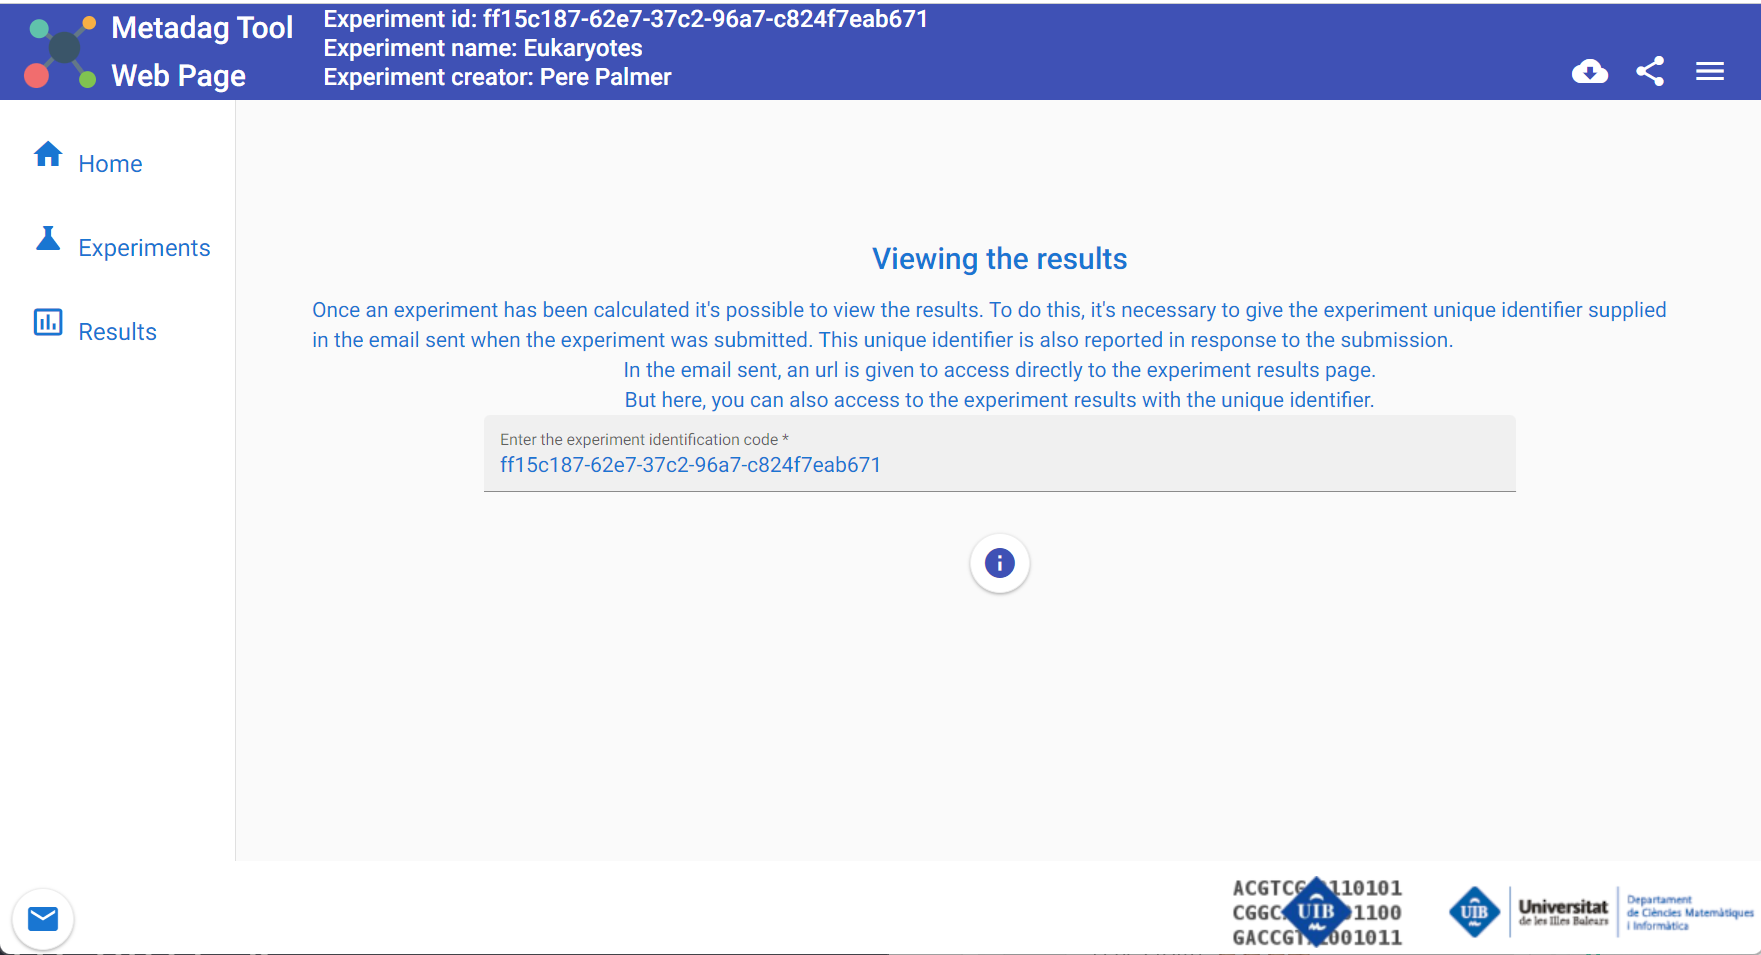
\includegraphics[width=5.87in,height=\textheight]{./figures/screen_1.png}

\bookmarksetup{startatroot}

\hypertarget{load-data-metadag-experiment}{%
\chapter{Load data MetaDag
experiment}\label{load-data-metadag-experiment}}

\begin{Shaded}
\begin{Highlighting}[]
\FunctionTok{library}\NormalTok{(tidyverse)}
\end{Highlighting}
\end{Shaded}

\begin{verbatim}
-- Attaching core tidyverse packages ------------------------ tidyverse 2.0.0 --
v dplyr     1.1.2     v readr     2.1.4
v forcats   1.0.0     v stringr   1.5.0
v ggplot2   3.4.2     v tibble    3.2.1
v lubridate 1.9.2     v tidyr     1.3.0
v purrr     1.0.1     
-- Conflicts ------------------------------------------ tidyverse_conflicts() --
x dplyr::filter() masks stats::filter()
x dplyr::lag()    masks stats::lag()
i Use the conflicted package (<http://conflicted.r-lib.org/>) to force all conflicts to become errors
\end{verbatim}

\begin{Shaded}
\begin{Highlighting}[]
\NormalTok{experiment}\OtherTok{=}
  \StringTok{"results\_ff15c187{-}62e7{-}37c2{-}96a7{-}c824f7eab671"}
\NormalTok{path\_exp}\OtherTok{=}\FunctionTok{paste0}\NormalTok{(}\StringTok{"data/"}\NormalTok{,experiment,}\StringTok{"/data/"}\NormalTok{)}
\FunctionTok{dir}\NormalTok{(path\_exp)}
\end{Highlighting}
\end{Shaded}

\begin{verbatim}
 [1] "Different_MBB.csv"                            
 [2] "Different_mDAG.csv"                           
 [3] "Global"                                       
 [4] "Individuals"                                  
 [5] "Results.csv"                                  
 [6] "Similarities_MBB_MSAMethod.csv"               
 [7] "Similarities_MBB_MunkresMethod.csv"           
 [8] "Similarities_mDAG_MSAMethod.csv"              
 [9] "Similarities_mDAG_MSAMethod_MunkresMethod.csv"
[10] "Similarities_mDAG_MunkresMethod.csv"          
[11] "Similarities_mDAG_MunkresMethod_MSAMethod.csv"
[12] "Similarities_mDAGOnReaction.csv"              
[13] "TaxonomyLevels"                               
\end{verbatim}

\begin{Shaded}
\begin{Highlighting}[]
\NormalTok{MBB}\OtherTok{=}\FunctionTok{read\_csv}\NormalTok{(}\FunctionTok{paste0}\NormalTok{(path\_exp,}\StringTok{"Different\_MBB.csv"}\NormalTok{),}\AttributeTok{show\_col\_types =} \ConstantTok{FALSE}\NormalTok{)}
\NormalTok{mDAG}\OtherTok{=}\FunctionTok{read\_csv}\NormalTok{(}\FunctionTok{paste0}\NormalTok{(path\_exp,}\StringTok{"Different\_mDAG.csv"}\NormalTok{),}\AttributeTok{show\_col\_types =} \ConstantTok{FALSE}\NormalTok{)}
\NormalTok{Results}\OtherTok{=}\FunctionTok{read\_csv}\NormalTok{(}\FunctionTok{paste0}\NormalTok{(path\_exp,}\StringTok{"Results.csv"}\NormalTok{),}\AttributeTok{show\_col\_types =} \ConstantTok{FALSE}\NormalTok{)}
\end{Highlighting}
\end{Shaded}

\hypertarget{mbb}{%
\section{MBB}\label{mbb}}

In this experiment \texttt{MBB} is a table with 5112 rows and 4106
columns.

\begin{Shaded}
\begin{Highlighting}[]
\FunctionTok{library}\NormalTok{(knitr)}
\FunctionTok{library}\NormalTok{(kableExtra)}
\end{Highlighting}
\end{Shaded}

\begin{verbatim}

Attaching package: 'kableExtra'
\end{verbatim}

\begin{verbatim}
The following object is masked from 'package:dplyr':

    group_rows
\end{verbatim}

\begin{Shaded}
\begin{Highlighting}[]
\CommentTok{\#add\_header\_above(c("a" = 5, "b" = 18,"last"=2752{-}23)) \%\textgreater{}\%}
\CommentTok{\# kable\_paper() \%\textgreater{}\%}
\FunctionTok{kable}\NormalTok{(MBB[}\DecValTok{1}\SpecialCharTok{:}\DecValTok{20}\NormalTok{,}\DecValTok{1}\SpecialCharTok{:}\DecValTok{30}\NormalTok{]) }\SpecialCharTok{\%\textgreater{}\%}   \FunctionTok{scroll\_box}\NormalTok{(}\AttributeTok{width =} \StringTok{"100\%"}\NormalTok{, }\AttributeTok{height =} \StringTok{"200px"}\NormalTok{)}
\end{Highlighting}
\end{Shaded}

\begin{tabular}{l|r|r|r|r|r|r|r|r|r|r|r|r|r|r|r|r|r|r|r|r|r|r|r|r|r|r|r|r|r}
\hline
MBB Id & natural & \#pathways & Protists & Fungi & Plants & Animals & Alveolates & Amoebozoa & Annelids & Arthropods & Ascomycetes & Basal angiosperms & Basidiomycetes & Brachiopodas & Cephalochordates & Choanoflagellates & Cnidarians & Cryptomonads & Echinoderms & Eudicots & Euglenozoa & Ferns & Flatworms & Green algae & Haptophyta & Hemichordates & Heterolobosea & Metamonada & Microsporidians\\
\hline
0 & 0 & 0 & 0 & 0 & 0 & 0 & 0 & 0 & 0 & 0 & 0 & 0 & 0 & 0 & 0 & 0 & 0 & 0 & 0 & 0 & 0 & 0 & 0 & 0 & 0 & 0 & 0 & 0 & 0\\
\hline
0.0 & 0 & 0 & 0 & 0 & 0 & 0 & 0 & 0 & 0 & 0 & 0 & 0 & 0 & 0 & 0 & 0 & 0 & 0 & 0 & 0 & 0 & 0 & 0 & 0 & 0 & 0 & 0 & 0 & 0\\
\hline
0.0.0 & 1 & 1 & 1 & 0 & 0 & 0 & 0 & 0 & 0 & 0 & 0 & 0 & 0 & 0 & 0 & 0 & 0 & 0 & 0 & 0 & 0 & 0 & 0 & 0 & 0 & 0 & 0 & 0 & 0\\
\hline
0.0.0.0 & 1 & 1 & 1 & 0 & 0 & 0 & 0 & 0 & 0 & 0 & 0 & 0 & 0 & 0 & 0 & 0 & 0 & 0 & 0 & 0 & 0 & 0 & 0 & 0 & 0 & 0 & 0 & 0 & 0\\
\hline
0.0.1 & 1 & 1 & 1 & 0 & 0 & 0 & 0 & 0 & 0 & 0 & 0 & 0 & 0 & 0 & 0 & 0 & 0 & 0 & 0 & 0 & 0 & 0 & 0 & 0 & 0 & 0 & 0 & 0 & 0\\
\hline
0.0.1.0 & 1 & 86 & 2 & 77 & 1 & 6 & 1 & 0 & 0 & 5 & 57 & 0 & 20 & 0 & 0 & 0 & 0 & 0 & 0 & 0 & 0 & 0 & 0 & 0 & 1 & 0 & 0 & 0 & 0\\
\hline
0.0.1.1 & 1 & 86 & 2 & 77 & 1 & 6 & 1 & 0 & 0 & 5 & 57 & 0 & 20 & 0 & 0 & 0 & 0 & 0 & 0 & 0 & 0 & 0 & 0 & 0 & 1 & 0 & 0 & 0 & 0\\
\hline
0.0.1.2 & 1 & 15 & 15 & 0 & 0 & 0 & 12 & 0 & 0 & 0 & 0 & 0 & 0 & 0 & 0 & 0 & 0 & 0 & 0 & 0 & 0 & 0 & 0 & 0 & 0 & 0 & 0 & 0 & 0\\
\hline
0.0.1.3 & 1 & 5 & 5 & 0 & 0 & 0 & 0 & 4 & 0 & 0 & 0 & 0 & 0 & 0 & 0 & 0 & 0 & 0 & 0 & 0 & 0 & 0 & 0 & 0 & 0 & 0 & 1 & 0 & 0\\
\hline
0.0.1.4 & 0 & 0 & 0 & 0 & 0 & 0 & 0 & 0 & 0 & 0 & 0 & 0 & 0 & 0 & 0 & 0 & 0 & 0 & 0 & 0 & 0 & 0 & 0 & 0 & 0 & 0 & 0 & 0 & 0\\
\hline
0.0.1.4.0 & 1 & 609 & 14 & 128 & 128 & 339 & 1 & 3 & 1 & 8 & 93 & 2 & 35 & 1 & 2 & 2 & 4 & 0 & 3 & 98 & 0 & 1 & 3 & 3 & 1 & 1 & 1 & 1 & 0\\
\hline
0.0.1.4.1 & 1 & 609 & 14 & 128 & 128 & 339 & 1 & 3 & 1 & 8 & 93 & 2 & 35 & 1 & 2 & 2 & 4 & 0 & 3 & 98 & 0 & 1 & 3 & 3 & 1 & 1 & 1 & 1 & 0\\
\hline
0.0.1.4.2 & 1 & 322 & 6 & 92 & 133 & 91 & 1 & 0 & 0 & 61 & 62 & 2 & 30 & 1 & 2 & 1 & 8 & 0 & 2 & 98 & 0 & 1 & 0 & 7 & 1 & 1 & 1 & 0 & 0\\
\hline
0.0.1.4.3 & 1 & 322 & 6 & 92 & 133 & 91 & 1 & 0 & 0 & 61 & 62 & 2 & 30 & 1 & 2 & 1 & 8 & 0 & 2 & 98 & 0 & 1 & 0 & 7 & 1 & 1 & 1 & 0 & 0\\
\hline
0.0.1.4.4 & 1 & 1 & 0 & 0 & 1 & 0 & 0 & 0 & 0 & 0 & 0 & 0 & 0 & 0 & 0 & 0 & 0 & 0 & 0 & 0 & 0 & 0 & 0 & 0 & 0 & 0 & 0 & 0 & 0\\
\hline
0.0.1.4.5 & 1 & 1 & 1 & 0 & 0 & 0 & 0 & 1 & 0 & 0 & 0 & 0 & 0 & 0 & 0 & 0 & 0 & 0 & 0 & 0 & 0 & 0 & 0 & 0 & 0 & 0 & 0 & 0 & 0\\
\hline
0.0.1.5 & 0 & 0 & 0 & 0 & 0 & 0 & 0 & 0 & 0 & 0 & 0 & 0 & 0 & 0 & 0 & 0 & 0 & 0 & 0 & 0 & 0 & 0 & 0 & 0 & 0 & 0 & 0 & 0 & 0\\
\hline
0.0.1.5.0 & 1 & 5 & 5 & 0 & 0 & 0 & 0 & 4 & 0 & 0 & 0 & 0 & 0 & 0 & 0 & 0 & 0 & 0 & 0 & 0 & 0 & 0 & 0 & 0 & 0 & 0 & 1 & 0 & 0\\
\hline
0.0.2 & 1 & 1 & 1 & 0 & 0 & 0 & 0 & 0 & 0 & 0 & 0 & 0 & 0 & 0 & 0 & 0 & 0 & 0 & 0 & 0 & 0 & 0 & 0 & 0 & 0 & 0 & 0 & 0 & 0\\
\hline
0.0.3 & 1 & 1 & 1 & 0 & 0 & 0 & 0 & 1 & 0 & 0 & 0 & 0 & 0 & 0 & 0 & 0 & 0 & 0 & 0 & 0 & 0 & 0 & 0 & 0 & 0 & 0 & 0 & 0 & 0\\
\hline
\end{tabular}

Manual columnas MBB

\begin{Shaded}
\begin{Highlighting}[]
\CommentTok{\#definition\_cols=data.frame(col\_number,col\_name,col,definition)}
\end{Highlighting}
\end{Shaded}

\hypertarget{mdag}{%
\section{mDAG}\label{mdag}}

Abstract/unique mDAG's in this experiment

\begin{Shaded}
\begin{Highlighting}[]
\FunctionTok{dim}\NormalTok{(mDAG)}
\end{Highlighting}
\end{Shaded}

\begin{verbatim}
[1]  884 5224
\end{verbatim}

\begin{Shaded}
\begin{Highlighting}[]
\FunctionTok{kable}\NormalTok{(mDAG[}\DecValTok{1}\SpecialCharTok{:}\DecValTok{20}\NormalTok{,}\DecValTok{1}\SpecialCharTok{:}\DecValTok{30}\NormalTok{]) }\SpecialCharTok{\%\textgreater{}\%}   \FunctionTok{scroll\_box}\NormalTok{(}\AttributeTok{width =} \StringTok{"100\%"}\NormalTok{, }\AttributeTok{height =} \StringTok{"200px"}\NormalTok{)}
\end{Highlighting}
\end{Shaded}

\begin{tabular}{l|r|r|r|r|r|r|r|r|r|r|r|r|r|r|r|r|r|r|r|r|r|r|r|r|r|r|r|r|r}
\hline
mDAG Id & \#Categories & Animals & Plants & Fungi & Protists & Alveolates & Amoebozoa & Annelids & Arthropods & Ascomycetes & Basal angiosperms & Basidiomycetes & Brachiopodas & Cephalochordates & Choanoflagellates & Cnidarians & Cryptomonads & Echinoderms & Eudicots & Euglenozoa & Ferns & Flatworms & Green algae & Haptophyta & Hemichordates & Heterolobosea & Metamonada & Microsporidians & Mollusks\\
\hline
0001 & 3 & 1 & 0 & 0 & 0 & 0 & 0 & 0 & 0 & 0 & 0 & 0 & 0 & 0 & 0 & 0 & 0 & 0 & 0 & 0 & 0 & 0 & 0 & 0 & 0 & 0 & 0 & 0 & 0\\
\hline
0002 & 2 & 0 & 0 & 1 & 0 & 0 & 0 & 0 & 0 & 0 & 0 & 1 & 0 & 0 & 0 & 0 & 0 & 0 & 0 & 0 & 0 & 0 & 0 & 0 & 0 & 0 & 0 & 0 & 0\\
\hline
0003 & 2 & 1 & 0 & 0 & 0 & 0 & 0 & 0 & 0 & 0 & 0 & 0 & 0 & 0 & 0 & 0 & 0 & 0 & 0 & 0 & 0 & 1 & 0 & 0 & 0 & 0 & 0 & 0 & 0\\
\hline
0004 & 3 & 1 & 0 & 0 & 0 & 0 & 0 & 0 & 0 & 0 & 0 & 0 & 0 & 0 & 0 & 0 & 0 & 0 & 0 & 0 & 0 & 0 & 0 & 0 & 0 & 0 & 0 & 0 & 0\\
\hline
0005 & 3 & 1 & 0 & 0 & 0 & 0 & 0 & 0 & 0 & 0 & 0 & 0 & 0 & 0 & 0 & 0 & 0 & 0 & 0 & 0 & 0 & 0 & 0 & 0 & 0 & 0 & 0 & 0 & 0\\
\hline
0006 & 3 & 0 & 1 & 0 & 0 & 0 & 0 & 0 & 0 & 0 & 0 & 0 & 0 & 0 & 0 & 0 & 0 & 0 & 1 & 0 & 0 & 0 & 0 & 0 & 0 & 0 & 0 & 0 & 0\\
\hline
0007 & 2 & 0 & 1 & 0 & 0 & 0 & 0 & 0 & 0 & 0 & 0 & 0 & 0 & 0 & 0 & 0 & 0 & 0 & 0 & 0 & 0 & 0 & 0 & 0 & 0 & 0 & 0 & 0 & 0\\
\hline
0008 & 3 & 0 & 1 & 0 & 0 & 0 & 0 & 0 & 0 & 0 & 0 & 0 & 0 & 0 & 0 & 0 & 0 & 0 & 0 & 0 & 0 & 0 & 0 & 0 & 0 & 0 & 0 & 0 & 0\\
\hline
0009 & 3 & 0 & 1 & 0 & 0 & 0 & 0 & 0 & 0 & 0 & 0 & 0 & 0 & 0 & 0 & 0 & 0 & 0 & 1 & 0 & 0 & 0 & 0 & 0 & 0 & 0 & 0 & 0 & 0\\
\hline
0010 & 3 & 1 & 0 & 0 & 0 & 0 & 0 & 0 & 0 & 0 & 0 & 0 & 0 & 0 & 0 & 0 & 0 & 0 & 0 & 0 & 0 & 0 & 0 & 0 & 0 & 0 & 0 & 0 & 0\\
\hline
0011 & 3 & 1 & 0 & 0 & 0 & 0 & 0 & 0 & 0 & 0 & 0 & 0 & 0 & 0 & 0 & 0 & 0 & 0 & 0 & 0 & 0 & 0 & 0 & 0 & 0 & 0 & 0 & 0 & 0\\
\hline
0012 & 3 & 0 & 0 & 0 & 1 & 0 & 0 & 0 & 0 & 0 & 0 & 0 & 0 & 0 & 0 & 0 & 0 & 0 & 0 & 0 & 0 & 0 & 0 & 0 & 0 & 0 & 1 & 0 & 0\\
\hline
0013 & 3 & 1 & 0 & 0 & 0 & 0 & 0 & 0 & 0 & 0 & 0 & 0 & 0 & 0 & 0 & 0 & 0 & 0 & 0 & 0 & 0 & 0 & 0 & 0 & 0 & 0 & 0 & 0 & 0\\
\hline
0014 & 3 & 0 & 0 & 0 & 1 & 1 & 0 & 0 & 0 & 0 & 0 & 0 & 0 & 0 & 0 & 0 & 0 & 0 & 0 & 0 & 0 & 0 & 0 & 0 & 0 & 0 & 0 & 0 & 0\\
\hline
0015 & 2 & 0 & 0 & 1 & 0 & 0 & 0 & 0 & 0 & 0 & 0 & 0 & 0 & 0 & 0 & 0 & 0 & 0 & 0 & 0 & 0 & 0 & 0 & 0 & 0 & 0 & 0 & 1 & 0\\
\hline
0016 & 3 & 0 & 0 & 0 & 1 & 0 & 1 & 0 & 0 & 0 & 0 & 0 & 0 & 0 & 0 & 0 & 0 & 0 & 0 & 0 & 0 & 0 & 0 & 0 & 0 & 0 & 0 & 0 & 0\\
\hline
0017 & 3 & 1 & 0 & 0 & 0 & 0 & 0 & 0 & 0 & 0 & 0 & 0 & 0 & 0 & 0 & 0 & 0 & 0 & 0 & 0 & 0 & 0 & 0 & 0 & 0 & 0 & 0 & 0 & 0\\
\hline
0018 & 3 & 1 & 0 & 0 & 0 & 0 & 0 & 0 & 0 & 0 & 0 & 0 & 0 & 0 & 0 & 0 & 0 & 0 & 0 & 0 & 0 & 0 & 0 & 0 & 0 & 0 & 0 & 0 & 0\\
\hline
0019 & 3 & 1 & 0 & 0 & 0 & 0 & 0 & 0 & 1 & 0 & 0 & 0 & 0 & 0 & 0 & 0 & 0 & 0 & 0 & 0 & 0 & 0 & 0 & 0 & 0 & 0 & 0 & 0 & 0\\
\hline
0020 & 3 & 1 & 0 & 0 & 0 & 0 & 0 & 0 & 0 & 0 & 0 & 0 & 0 & 0 & 0 & 0 & 0 & 0 & 0 & 0 & 0 & 0 & 0 & 0 & 0 & 0 & 0 & 0 & 0\\
\hline
\end{tabular}

\begin{Shaded}
\begin{Highlighting}[]
\FunctionTok{dim}\NormalTok{(mDAG)}
\end{Highlighting}
\end{Shaded}

\begin{verbatim}
[1]  884 5224
\end{verbatim}

\begin{Shaded}
\begin{Highlighting}[]
\FunctionTok{names}\NormalTok{(mDAG)[}\DecValTok{1}\SpecialCharTok{:}\DecValTok{6}\NormalTok{]}
\end{Highlighting}
\end{Shaded}

\begin{verbatim}
[1] "mDAG Id"     "#Categories" "Animals"     "Plants"      "Fungi"      
[6] "Protists"   
\end{verbatim}

\begin{Shaded}
\begin{Highlighting}[]
\FunctionTok{names}\NormalTok{(mDAG)[}\DecValTok{7}\SpecialCharTok{:}\NormalTok{(}\FunctionTok{dim}\NormalTok{(mDAG)[}\DecValTok{2}\NormalTok{]}\SpecialCharTok{{-}}\DecValTok{1150}\NormalTok{)]}\CommentTok{\# 28 to 1213  code MBB: 1 if MBB in mDAG 0 }
\end{Highlighting}
\end{Shaded}

\begin{verbatim}
   [1] "Alveolates"                 "Amoebozoa"                 
   [3] "Annelids"                   "Arthropods"                
   [5] "Ascomycetes"                "Basal angiosperms"         
   [7] "Basidiomycetes"             "Brachiopodas"              
   [9] "Cephalochordates"           "Choanoflagellates"         
  [11] "Cnidarians"                 "Cryptomonads"              
  [13] "Echinoderms"                "Eudicots"                  
  [15] "Euglenozoa"                 "Ferns"                     
  [17] "Flatworms"                  "Green algae"               
  [19] "Haptophyta"                 "Hemichordates"             
  [21] "Heterolobosea"              "Metamonada"                
  [23] "Microsporidians"            "Mollusks"                  
  [25] "Monocots"                   "Mosses"                    
  [27] "Nematodes"                  "Placozoans"                
  [29] "Poriferans"                 "Red algae"                 
  [31] "Stramenopiles"              "Tunicates"                 
  [33] "Vertebrates"                "Acanthamoeba"              
  [35] "Acanthus family"            "Amaranth family"           
  [37] "Amborella family"           "Amphibians"                
  [39] "Apicomplexans"              "Asparagus family"          
  [41] "Banana family"              "Beech family"              
  [43] "Birds"                      "Bittersweet family"        
  [45] "Buckthorn family"           "Caper family"              
  [47] "Cartilaginous fishes"       "Chelicerates"              
  [49] "Ciliates"                   "Crustaceans"               
  [51] "Cucumber family"            "Daisy family"              
  [53] "Diatoms"                    "Dictyostelia"              
  [55] "Dinoflagellates"            "Diplomonads"               
  [57] "Dothideomycetes"            "Entamoeba"                 
  [59] "Eurotiomycetes"             "Eustigmatophytes"          
  [61] "Fishes"                     "Ginger family"             
  [63] "Grape family"               "Grass family"              
  [65] "Insects"                    "Kinetoplasts"              
  [67] "Leotiomycetes"              "Lopseed family"            
  [69] "Lotus family"               "Mallow family"             
  [71] "Mammals"                    "Mint family"               
  [73] "Morning-glory family"       "Mulberry family"           
  [75] "Mustard family"             "Myrtle family"             
  [77] "Nightshade family"          "Olive family"              
  [79] "Oomycetes"                  "Orchid family"             
  [81] "Palm family"                "Papaya family"             
  [83] "Parsley family"             "Pea family"                
  [85] "Pelagophytes"               "Pezizomycetes"             
  [87] "Poppy family"               "Protea family"             
  [89] "Reptiles"                   "Rose family"               
  [91] "Rue family"                 "Saccharomycetes"           
  [93] "Schizosaccharomycetes"      "Sesame family"             
  [95] "Sordariomycetes"            "Spurge family"             
  [97] "Sumac family"               "Tea family"                
  [99] "Tetramitia"                 "Trichomonads"              
 [101] "Walnut family"              "Water-lily family"         
 [103] "Willow family"              "#MMB"                      
 [105] "0"                          "0.0"                       
 [107] "0.0.0"                      "0.0.0.0"                   
 [109] "0.0.1"                      "0.0.1.0"                   
 [111] "0.0.1.1"                    "0.0.1.2"                   
 [113] "0.0.1.3"                    "0.0.1.4"                   
 [115] "0.0.1.4.0"                  "0.0.1.4.1"                 
 [117] "0.0.1.4.2"                  "0.0.1.4.3"                 
 [119] "0.0.1.4.4"                  "0.0.1.4.5"                 
 [121] "0.0.1.5"                    "0.0.1.5.0"                 
 [123] "0.0.2"                      "0.0.3"                     
 [125] "0.0.3.0"                    "0.0.4"                     
 [127] "0.0.4.0"                    "0.0.4.0.0"                 
 [129] "0.0.4.0.0.0"                "0.0.4.1"                   
 [131] "0.0.5"                      "0.0.6"                     
 [133] "0.0.7"                      "0.0.8"                     
 [135] "0.0.9"                      "0.0.9.0"                   
 [137] "0.0.10"                     "0.0.11"                    
 [139] "0.0.11.0"                   "0.0.11.1"                  
 [141] "0.0.11.2"                   "0.0.11.3"                  
 [143] "0.0.11.4"                   "0.0.11.5"                  
 [145] "0.0.11.6"                   "0.0.11.7"                  
 [147] "0.0.11.8"                   "0.0.11.9"                  
 [149] "0.0.11.10"                  "0.0.11.11"                 
 [151] "0.0.12"                     "0.0.13"                    
 [153] "0.0.14"                     "0.0.14.0"                  
 [155] "0.0.14.0.0"                 "0.0.14.0.1"                
 [157] "0.0.14.0.1.0"               "0.0.14.0.1.1"              
 [159] "0.0.14.1"                   "0.0.15"                    
 [161] "0.0.17"                     "0.0.17.0"                  
 [163] "0.0.19"                     "0.0.20"                    
 [165] "0.0.21"                     "0.0.21.0"                  
 [167] "0.0.21.0.0"                 "0.0.21.1"                  
 [169] "0.0.21.2"                   "0.0.21.2.0"                
 [171] "0.0.21.2.1"                 "0.0.21.2.2"                
 [173] "0.0.21.2.3"                 "0.0.21.2.3.0"              
 [175] "0.0.21.2.3.0.0"             "0.0.21.2.4"                
 [177] "0.0.21.2.5"                 "0.0.22"                    
 [179] "0.0.22.0"                   "0.0.23"                    
 [181] "0.0.24"                     "0.0.25"                    
 [183] "0.0.25.0"                   "0.0.25.0.0"                
 [185] "0.0.25.0.1"                 "0.0.25.1"                  
 [187] "0.0.25.2"                   "0.0.25.3"                  
 [189] "0.0.25.4"                   "0.0.25.4.0"                
 [191] "0.0.31"                     "0.0.32"                    
 [193] "0.0.32.0"                   "0.0.32.1"                  
 [195] "0.0.35"                     "0.0.35.0"                  
 [197] "0.0.35.0.0"                 "0.0.35.1"                  
 [199] "0.0.36"                     "0.0.37"                    
 [201] "0.0.38"                     "0.0.40"                    
 [203] "0.0.41"                     "0.0.42"                    
 [205] "0.0.43"                     "0.0.43.0"                  
 [207] "0.0.47"                     "0.0.47.0"                  
 [209] "0.0.48"                     "0.0.48.0"                  
 [211] "0.0.49"                     "0.0.50"                    
 [213] "0.0.51"                     "0.0.51.0"                  
 [215] "0.0.51.0.0"                 "0.0.51.0.0.0"              
 [217] "0.0.51.0.0.1"               "0.0.51.1"                  
 [219] "0.0.51.2"                   "0.0.51.2.0"                
 [221] "0.0.51.2.0.0"               "0.0.51.2.0.1"              
 [223] "0.0.51.2.1"                 "0.0.51.2.1.0"              
 [225] "0.0.51.2.1.0.0"             "0.0.51.2.1.0.0.0"          
 [227] "0.0.52"                     "0.0.52.0"                  
 [229] "0.0.52.0.0"                 "0.0.53"                    
 [231] "0.0.53.0"                   "0.0.53.0.0"                
 [233] "0.0.54"                     "0.0.54.0"                  
 [235] "0.0.54.1"                   "0.0.54.2"                  
 [237] "0.0.54.2.0"                 "0.0.55"                    
 [239] "0.0.57"                     "0.0.57.0"                  
 [241] "0.0.57.1"                   "0.0.58"                    
 [243] "0.0.58.0"                   "0.0.58.0.0"                
 [245] "0.0.58.0.0.0"               "0.0.58.0.0.1"              
 [247] "0.0.58.0.0.2"               "0.0.58.0.0.2.0"            
 [249] "0.0.58.0.0.3"               "0.0.58.0.0.4"              
 [251] "0.0.58.0.0.5"               "0.0.58.0.0.5.0"            
 [253] "0.0.58.0.0.5.1"             "0.0.58.0.0.5.2"            
 [255] "0.0.58.0.0.6"               "0.0.58.0.0.7"              
 [257] "0.0.58.0.0.7.0"             "0.0.58.0.0.7.1"            
 [259] "0.0.58.0.0.7.2"             "0.0.58.0.0.7.3"            
 [261] "0.0.58.0.1"                 "0.0.58.0.1.0"              
 [263] "0.0.58.0.1.0.0"             "0.0.58.0.1.0.1"            
 [265] "0.0.58.0.2"                 "0.0.62"                    
 [267] "0.0.62.0"                   "0.0.62.1"                  
 [269] "0.0.62.1.0"                 "0.0.62.1.1"                
 [271] "0.0.62.1.2"                 "0.0.62.2"                  
 [273] "0.0.62.3"                   "0.0.62.3.0"                
 [275] "0.0.63"                     "0.0.63.0"                  
 [277] "0.0.63.1"                   "0.0.63.2"                  
 [279] "0.0.63.3"                   "0.0.63.4"                  
 [281] "0.0.63.5"                   "0.0.63.6"                  
 [283] "0.0.64"                     "0.0.65"                    
 [285] "0.0.67"                     "0.0.70"                    
 [287] "0.0.71"                     "0.0.71.0"                  
 [289] "0.0.71.1"                   "0.0.75"                    
 [291] "0.0.75.0"                   "0.0.75.0.0"                
 [293] "0.0.75.1"                   "0.0.76"                    
 [295] "0.0.76.0"                   "0.0.76.0.0"                
 [297] "0.0.76.0.0.0"               "0.0.76.0.0.1"              
 [299] "0.0.76.0.0.1.0"             "0.0.76.0.0.1.0.0"          
 [301] "0.0.76.0.0.1.0.1"           "0.0.76.0.0.1.1"            
 [303] "0.0.76.0.1"                 "0.0.76.0.1.0"              
 [305] "0.0.76.0.1.1"               "0.0.76.0.2"                
 [307] "0.0.76.1"                   "0.0.76.1.0"                
 [309] "0.0.76.1.0.0"               "0.0.76.1.0.0.0"            
 [311] "0.0.76.1.1"                 "0.0.76.2"                  
 [313] "0.0.76.3"                   "0.0.76.3.0"                
 [315] "0.0.76.3.0.0"               "0.0.76.3.0.0.0"            
 [317] "0.0.76.3.0.1"               "0.0.77"                    
 [319] "0.0.78"                     "0.0.78.0"                  
 [321] "0.0.78.0.0"                 "0.0.78.1"                  
 [323] "0.0.78.2"                   "0.0.78.3"                  
 [325] "0.0.78.4"                   "0.0.78.5"                  
 [327] "0.0.79"                     "0.0.80"                    
 [329] "0.0.80.0"                   "0.0.80.0.0"                
 [331] "0.0.80.0.0.0"               "0.0.80.1"                  
 [333] "0.0.80.2"                   "0.0.81"                    
 [335] "0.0.81.0"                   "0.0.81.1"                  
 [337] "0.0.83"                     "0.0.83.0"                  
 [339] "0.0.85"                     "0.0.85.0"                  
 [341] "0.0.85.0.0"                 "0.0.85.1"                  
 [343] "0.0.85.2"                   "0.0.85.3"                  
 [345] "0.0.87"                     "0.0.87.0"                  
 [347] "0.0.87.1"                   "0.0.89"                    
 [349] "0.0.89.0"                   "0.0.89.0.0"                
 [351] "0.0.90"                     "0.0.90.0"                  
 [353] "0.0.90.0.0"                 "0.0.91"                    
 [355] "0.0.91.0"                   "0.0.94"                    
 [357] "0.0.94.0"                   "0.0.94.0.0"                
 [359] "0.0.94.1"                   "0.0.94.2"                  
 [361] "0.0.94.2.0"                 "0.0.94.2.0.0"              
 [363] "0.0.94.2.0.0.0"             "0.0.94.2.0.0.0.0"          
 [365] "0.0.94.2.0.0.0.1"           "0.0.94.2.0.0.0.2"          
 [367] "0.0.94.2.0.0.1"             "0.0.94.2.0.0.1.0"          
 [369] "0.0.94.2.0.1"               "0.0.94.2.0.1.0"            
 [371] "0.0.94.2.0.1.1"             "0.0.94.2.0.1.2"            
 [373] "0.0.94.2.0.2"               "0.0.94.2.1"                
 [375] "0.0.97"                     "0.0.97.0"                  
 [377] "0.0.97.1"                   "0.0.98"                    
 [379] "0.0.99"                     "0.0.99.0"                  
 [381] "0.0.100"                    "0.0.100.0"                 
 [383] "0.0.100.0.0"                "0.0.101"                   
 [385] "0.0.101.0"                  "0.0.101.0.0"               
 [387] "0.0.101.0.0.0"              "0.0.101.0.0.1"             
 [389] "0.0.101.0.1"                "0.0.101.0.1.0"             
 [391] "0.0.101.0.1.0.0"            "0.0.101.0.1.0.0.0"         
 [393] "0.0.101.0.1.0.0.1"          "0.0.101.0.1.0.0.1.0"       
 [395] "0.0.101.0.1.0.0.2"          "0.0.101.0.1.0.0.3"         
 [397] "0.0.101.0.1.0.0.4"          "0.0.101.0.1.0.1"           
 [399] "0.0.101.0.1.0.1.0"          "0.0.101.0.1.0.1.0.0"       
 [401] "0.0.101.0.1.0.1.0.1"        "0.0.101.0.1.0.1.0.2"       
 [403] "0.0.101.0.1.0.1.0.2.0"      "0.0.101.0.1.0.1.1"         
 [405] "0.0.102"                    "0.0.102.0"                 
 [407] "0.0.102.0.0"                "0.0.102.0.0.0"             
 [409] "0.0.102.0.0.0.0"            "0.0.102.0.0.1"             
 [411] "0.0.102.0.0.1.0"            "0.0.102.0.1"               
 [413] "0.0.102.0.1.0"              "0.0.102.0.1.0.0"           
 [415] "0.0.102.1"                  "0.0.102.1.0"               
 [417] "0.0.102.1.0.0"              "0.0.102.1.1"               
 [419] "0.0.102.2"                  "0.0.102.2.0"               
 [421] "0.0.102.3"                  "0.0.102.3.0"               
 [423] "0.0.102.4"                  "0.0.103"                   
 [425] "0.0.103.0"                  "0.0.103.0.0"               
 [427] "0.0.104"                    "0.0.104.0"                 
 [429] "0.0.104.0.0"                "0.0.104.0.0.0"             
 [431] "0.0.104.0.0.1"              "0.0.104.0.1"               
 [433] "0.0.104.0.2"                "0.0.104.0.2.0"             
 [435] "0.0.105"                    "0.0.105.0"                 
 [437] "0.0.105.0.0"                "0.0.105.1"                 
 [439] "0.0.105.1.0"                "0.0.107"                   
 [441] "0.0.107.0"                  "0.0.108"                   
 [443] "0.0.109"                    "0.0.109.0"                 
 [445] "0.0.109.1"                  "0.0.110"                   
 [447] "0.0.111"                    "0.0.111.0"                 
 [449] "0.0.111.1"                  "0.0.111.2"                 
 [451] "0.0.112"                    "0.0.115"                   
 [453] "0.0.116"                    "0.0.117"                   
 [455] "0.0.117.0"                  "0.0.117.0.0"               
 [457] "0.0.119"                    "0.0.119.0"                 
 [459] "0.0.121"                    "0.0.121.0"                 
 [461] "0.0.123"                    "0.0.123.0"                 
 [463] "0.0.123.0.0"                "0.0.123.0.0.0"             
 [465] "0.0.123.1"                  "0.0.123.1.0"               
 [467] "0.0.123.1.0.0"              "0.0.123.1.0.0.0"           
 [469] "0.0.123.1.0.0.1"            "0.0.123.1.0.1"             
 [471] "0.0.123.1.1"                "0.0.123.1.1.0"             
 [473] "0.0.124"                    "0.0.128"                   
 [475] "0.0.128.0"                  "0.0.128.0.0"               
 [477] "0.0.128.0.0.0"              "0.0.128.0.0.0.0"           
 [479] "0.0.128.0.0.1"              "0.0.128.0.0.2"             
 [481] "0.0.128.0.0.3"              "0.0.128.0.1"               
 [483] "0.0.128.0.1.0"              "0.0.128.1"                 
 [485] "0.0.129"                    "0.0.131"                   
 [487] "0.0.132"                    "0.0.132.0"                 
 [489] "0.0.132.1"                  "0.0.132.2"                 
 [491] "0.0.133"                    "0.0.139"                   
 [493] "0.0.139.0"                  "0.0.139.1"                 
 [495] "0.0.139.2"                  "0.0.146"                   
 [497] "0.0.146.0"                  "0.0.146.0.0"               
 [499] "0.0.146.0.0.0"              "0.0.146.0.0.0.0"           
 [501] "0.0.146.0.0.0.0.0"          "0.0.146.0.0.0.0.1"         
 [503] "0.0.146.0.0.0.1"            "0.0.146.0.0.0.1.0"         
 [505] "0.0.146.0.0.0.1.0.0"        "0.0.146.0.0.1"             
 [507] "0.0.146.0.0.1.0"            "0.0.146.0.0.1.0.0"         
 [509] "0.0.146.0.0.1.0.1"          "0.0.146.0.1"               
 [511] "0.0.146.0.1.0"              "0.0.146.0.2"               
 [513] "0.0.146.1"                  "0.0.146.1.0"               
 [515] "0.0.146.1.0.0"              "0.0.146.1.0.0.0"           
 [517] "0.0.146.1.0.0.0.0"          "0.0.146.1.0.0.1"           
 [519] "0.0.146.1.0.1"              "0.0.146.1.0.1.0"           
 [521] "0.0.146.1.0.2"              "0.0.146.1.1"               
 [523] "0.0.146.1.1.0"              "0.0.146.1.1.0.0"           
 [525] "0.0.146.1.2"                "0.0.146.1.2.0"             
 [527] "0.0.146.1.3"                "0.0.146.2"                 
 [529] "0.0.146.2.0"                "0.0.146.3"                 
 [531] "0.0.146.3.0"                "0.0.146.4"                 
 [533] "0.0.148"                    "0.0.150"                   
 [535] "0.0.152"                    "0.0.153"                   
 [537] "0.0.154"                    "0.0.155"                   
 [539] "0.0.156"                    "0.0.157"                   
 [541] "0.0.157.0"                  "0.0.161"                   
 [543] "0.0.162"                    "0.0.163"                   
 [545] "0.0.164"                    "0.0.167"                   
 [547] "0.0.167.0"                  "0.0.167.1"                 
 [549] "0.0.167.2"                  "0.0.167.3"                 
 [551] "0.0.167.4"                  "0.0.167.5"                 
 [553] "0.0.167.6"                  "0.0.167.6.0"               
 [555] "0.0.167.6.1"                "0.0.167.7"                 
 [557] "0.0.172"                    "0.0.174"                   
 [559] "0.0.175"                    "0.0.175.0"                 
 [561] "0.0.175.0.0"                "0.0.175.0.0.0"             
 [563] "0.0.175.0.1"                "0.0.175.0.1.0"             
 [565] "0.0.175.0.2"                "0.0.175.1"                 
 [567] "0.0.175.1.0"                "0.0.175.1.0.0"             
 [569] "0.0.175.1.0.0.0"            "0.0.175.2"                 
 [571] "0.0.178"                    "0.0.179"                   
 [573] "0.0.184"                    "0.0.184.0"                 
 [575] "0.0.184.1"                  "0.0.185"                   
 [577] "0.0.185.0"                  "0.0.187"                   
 [579] "0.0.187.0"                  "0.0.188"                   
 [581] "0.0.188.0"                  "0.0.190"                   
 [583] "0.0.190.0"                  "0.0.190.1"                 
 [585] "0.0.190.2"                  "0.0.190.2.0"               
 [587] "0.0.190.2.1"                "0.0.193"                   
 [589] "0.0.193.0"                  "0.0.196"                   
 [591] "0.0.197"                    "0.0.199"                   
 [593] "0.0.199.0"                  "0.0.199.0.0"               
 [595] "0.0.199.0.0.0"              "0.0.200"                   
 [597] "0.0.200.0"                  "0.0.200.0.0"               
 [599] "0.0.200.0.1"                "0.0.200.1"                 
 [601] "0.0.201"                    "0.0.201.0"                 
 [603] "0.0.201.0.0"                "0.0.201.0.1"               
 [605] "0.0.201.1"                  "0.0.202"                   
 [607] "0.0.202.0"                  "0.0.202.0.0"               
 [609] "0.0.202.0.1"                "0.0.202.1"                 
 [611] "0.0.203"                    "0.0.203.0"                 
 [613] "0.0.203.0.0"                "0.0.203.0.1"               
 [615] "0.0.203.1"                  "0.0.206"                   
 [617] "0.0.206.0"                  "0.0.210"                   
 [619] "0.0.210.0"                  "0.0.210.0.0"               
 [621] "0.0.210.0.0.0"              "0.0.210.0.0.1"             
 [623] "0.0.210.0.1"                "0.0.210.0.1.0"             
 [625] "0.0.210.0.1.0.0"            "0.0.210.0.1.0.1"           
 [627] "0.0.210.0.1.0.1.0"          "0.0.210.0.1.0.2"           
 [629] "0.0.210.0.1.1"              "0.0.210.1"                 
 [631] "0.0.210.1.0"                "0.0.210.1.0.0"             
 [633] "0.0.212"                    "0.0.212.0"                 
 [635] "0.0.214"                    "0.0.214.0"                 
 [637] "0.0.215"                    "0.0.215.0"                 
 [639] "0.0.215.1"                  "0.0.215.2"                 
 [641] "0.0.215.3"                  "0.0.215.4"                 
 [643] "0.0.215.5"                  "0.0.220"                   
 [645] "0.0.220.0"                  "0.0.220.0.0"               
 [647] "0.0.220.0.1"                "0.0.222"                   
 [649] "0.0.223"                    "0.0.226"                   
 [651] "0.0.226.0"                  "0.0.231"                   
 [653] "0.0.231.0"                  "0.0.231.0.0"               
 [655] "0.0.231.0.0.0"              "0.0.231.0.1"               
 [657] "0.0.231.0.1.0"              "0.0.231.1"                 
 [659] "0.0.231.1.0"                "0.0.231.1.0.0"             
 [661] "0.0.234"                    "0.0.234.0"                 
 [663] "0.0.234.0.0"                "0.0.234.0.0.0"             
 [665] "0.0.234.0.0.1"              "0.0.234.0.1"               
 [667] "0.0.234.0.1.0"              "0.0.234.0.2"               
 [669] "0.0.234.1"                  "0.0.234.1.0"               
 [671] "0.0.234.1.0.0"              "0.0.237"                   
 [673] "0.0.238"                    "0.0.239"                   
 [675] "0.0.240"                    "0.0.242"                   
 [677] "0.0.242.0"                  "0.0.243"                   
 [679] "0.0.243.0"                  "0.0.244"                   
 [681] "0.0.245"                    "0.0.246"                   
 [683] "0.0.249"                    "0.0.249.0"                 
 [685] "0.0.249.0.0"                "0.0.249.0.0.0"             
 [687] "0.0.249.1"                  "0.0.255"                   
 [689] "0.0.256"                    "0.0.260"                   
 [691] "0.0.260.0"                  "0.0.260.0.0"               
 [693] "0.0.261"                    "0.0.263"                   
 [695] "0.0.264"                    "0.0.264.0"                 
 [697] "0.0.266"                    "0.0.266.0"                 
 [699] "0.0.266.0.0"                "0.0.266.0.1"               
 [701] "0.0.267"                    "0.0.272"                   
 [703] "0.0.272.0"                  "0.0.275"                   
 [705] "0.0.275.0"                  "0.0.277"                   
 [707] "0.0.279"                    "0.0.280"                   
 [709] "0.0.281"                    "0.0.282"                   
 [711] "0.0.287"                    "0.0.301"                   
 [713] "0.0.301.0"                  "0.0.303"                   
 [715] "0.0.303.0"                  "0.0.303.1"                 
 [717] "0.0.303.1.0"                "0.0.303.1.1"               
 [719] "0.0.305"                    "0.0.305.0"                 
 [721] "0.0.305.1"                  "0.0.305.2"                 
 [723] "0.0.305.3"                  "0.0.306"                   
 [725] "0.0.306.0"                  "0.0.306.0.0"               
 [727] "0.0.306.1"                  "0.0.308"                   
 [729] "0.0.308.0"                  "0.0.309"                   
 [731] "0.0.309.0"                  "0.0.309.0.0"               
 [733] "0.0.309.0.1"                "0.0.309.1"                 
 [735] "0.0.311"                    "0.0.311.0"                 
 [737] "0.0.312"                    "0.0.312.0"                 
 [739] "0.0.312.0.0"                "0.0.314"                   
 [741] "0.0.314.0"                  "0.0.314.0.0"               
 [743] "0.0.314.1"                  "0.0.315"                   
 [745] "0.0.315.0"                  "0.0.315.0.0"               
 [747] "0.0.315.1"                  "0.0.315.1.0"               
 [749] "0.0.315.2"                  "0.0.315.2.0"               
 [751] "0.0.320"                    "0.0.322"                   
 [753] "0.0.323"                    "0.0.324"                   
 [755] "0.0.325"                    "0.0.326"                   
 [757] "0.0.326.0"                  "0.0.326.0.0"               
 [759] "0.0.327"                    "0.0.327.0"                 
 [761] "0.0.327.0.0"                "0.0.328"                   
 [763] "0.0.328.0"                  "0.0.328.0.0"               
 [765] "0.0.331"                    "0.0.332"                   
 [767] "0.0.334"                    "0.0.334.0"                 
 [769] "0.0.334.0.0"                "0.0.335"                   
 [771] "0.0.335.0"                  "0.0.335.0.0"               
 [773] "0.0.335.0.1"                "0.0.335.1"                 
 [775] "0.0.336"                    "0.0.337"                   
 [777] "0.0.338"                    "0.0.339"                   
 [779] "0.0.340"                    "0.0.341"                   
 [781] "0.0.342"                    "0.0.349"                   
 [783] "0.0.349.0"                  "0.0.349.0.0"               
 [785] "0.0.349.1"                  "0.0.351"                   
 [787] "0.0.351.0"                  "0.0.351.0.0"               
 [789] "0.0.352"                    "0.0.352.0"                 
 [791] "0.0.352.0.0"                "0.0.353"                   
 [793] "0.0.353.0"                  "0.0.353.0.0"               
 [795] "0.0.354"                    "0.0.354.0"                 
 [797] "0.0.354.0.0"                "0.0.355"                   
 [799] "0.0.356"                    "0.0.357"                   
 [801] "0.0.358"                    "0.0.358.0"                 
 [803] "0.0.360"                    "0.0.361"                   
 [805] "0.0.361.0"                  "0.0.361.0.0"               
 [807] "0.0.361.0.1"                "0.0.361.1"                 
 [809] "0.0.361.1.0"                "0.0.363"                   
 [811] "0.0.363.0"                  "0.0.365"                   
 [813] "0.0.366"                    "0.0.367"                   
 [815] "0.0.372"                    "0.0.376"                   
 [817] "0.0.378"                    "0.0.378.0"                 
 [819] "0.0.378.1"                  "0.0.381"                   
 [821] "0.0.381.0"                  "0.0.381.1"                 
 [823] "0.0.381.2"                  "0.0.382"                   
 [825] "0.0.382.0"                  "0.0.382.0.0"               
 [827] "0.0.382.1"                  "0.0.384"                   
 [829] "0.0.384.0"                  "0.0.384.1"                 
 [831] "0.0.385"                    "0.0.385.0"                 
 [833] "0.0.385.1"                  "0.0.386"                   
 [835] "0.0.386.0"                  "0.0.386.1"                 
 [837] "0.0.387"                    "0.0.387.0"                 
 [839] "0.0.387.1"                  "0.0.388"                   
 [841] "0.0.390"                    "0.0.391"                   
 [843] "0.0.391.0"                  "0.0.391.0.0"               
 [845] "0.0.391.0.1"                "0.0.391.1"                 
 [847] "0.0.391.1.0"                "0.0.391.1.1"               
 [849] "0.0.392"                    "0.0.392.0"                 
 [851] "0.0.403"                    "0.0.404"                   
 [853] "0.0.404.0"                  "0.0.407"                   
 [855] "0.0.407.0"                  "0.0.407.1"                 
 [857] "0.0.412"                    "0.0.412.0"                 
 [859] "0.0.414"                    "0.0.416"                   
 [861] "0.0.420"                    "0.0.421"                   
 [863] "0.0.422"                    "0.0.422.0"                 
 [865] "0.0.424"                    "0.0.426"                   
 [867] "0.0.429"                    "0.0.430"                   
 [869] "0.0.431"                    "0.0.432"                   
 [871] "0.0.433"                    "0.0.434"                   
 [873] "0.0.435"                    "0.0.436"                   
 [875] "0.0.441"                    "0.0.442"                   
 [877] "0.0.443"                    "0.0.443.0"                 
 [879] "0.0.444"                    "0.0.447"                   
 [881] "0.0.451"                    "0.0.452"                   
 [883] "0.0.452.0"                  "0.0.454"                   
 [885] "0.0.455"                    "0.0.456"                   
 [887] "0.0.457"                    "0.0.462"                   
 [889] "0.0.465"                    "0.0.469"                   
 [891] "0.0.469.0"                  "0.0.470"                   
 [893] "0.0.470.0"                  "0.0.471"                   
 [895] "0.0.471.0"                  "0.0.474"                   
 [897] "0.0.476"                    "0.0.478"                   
 [899] "0.0.478.0"                  "0.0.478.1"                 
 [901] "0.0.481"                    "0.0.484"                   
 [903] "0.0.491"                    "0.0.492"                   
 [905] "0.0.493"                    "0.0.494"                   
 [907] "0.0.495"                    "0.0.497"                   
 [909] "0.0.498"                    "0.0.499"                   
 [911] "0.0.500"                    "0.0.501"                   
 [913] "0.0.502"                    "0.0.503"                   
 [915] "0.0.506"                    "0.0.506.0"                 
 [917] "0.0.506.1"                  "0.0.508"                   
 [919] "0.0.510"                    "0.0.510.0"                 
 [921] "0.0.510.1"                  "0.0.512"                   
 [923] "0.0.515"                    "0.0.515.0"                 
 [925] "0.0.517"                    "0.0.518"                   
 [927] "0.0.520"                    "0.0.525"                   
 [929] "0.0.529"                    "0.0.533"                   
 [931] "0.0.537"                    "0.0.538"                   
 [933] "0.0.538.0"                  "0.0.538.1"                 
 [935] "0.0.539"                    "0.0.549"                   
 [937] "0.0.552"                    "0.0.553"                   
 [939] "0.0.554"                    "0.0.556"                   
 [941] "0.0.558"                    "0.0.560"                   
 [943] "0.0.562"                    "0.0.563"                   
 [945] "0.0.564"                    "0.0.565"                   
 [947] "0.0.566"                    "0.0.567"                   
 [949] "0.0.576"                    "0.0.577"                   
 [951] "0.0.578"                    "0.0.581"                   
 [953] "0.0.584"                    "0.0.586"                   
 [955] "0.0.605"                    "0.0.608"                   
 [957] "0.0.609"                    "0.0.612"                   
 [959] "0.0.617"                    "0.0.618"                   
 [961] "0.0.619"                    "0.0.620"                   
 [963] "0.0.621"                    "0.0.622"                   
 [965] "0.0.623"                    "0.0.624"                   
 [967] "0.0.626"                    "0.0.627"                   
 [969] "0.0.628"                    "0.0.631"                   
 [971] "0.0.632"                    "0.0.633"                   
 [973] "0.0.634"                    "0.0.635"                   
 [975] "0.0.636"                    "0.0.637"                   
 [977] "0.0.638"                    "0.0.641"                   
 [979] "0.0.643"                    "0.0.644"                   
 [981] "0.0.645"                    "0.0.646"                   
 [983] "0.0.647"                    "0.0.648"                   
 [985] "0.0.649"                    "0.0.651"                   
 [987] "0.0.652"                    "0.0.653"                   
 [989] "0.0.654"                    "0.0.655"                   
 [991] "0.0.656"                    "0.0.658"                   
 [993] "0.0.659"                    "0.0.660"                   
 [995] "0.0.661"                    "0.0.666"                   
 [997] "0.0.669"                    "0.0.670"                   
 [999] "0.0.671"                    "0.0.672"                   
[1001] "0.0.673"                    "0.0.674"                   
[1003] "0.0.675"                    "0.0.676"                   
[1005] "0.0.677"                    "0.0.678"                   
[1007] "0.0.682"                    "0.0.684"                   
[1009] "0.0.685"                    "0.0.686"                   
[1011] "0.0.687"                    "0.0.688"                   
[1013] "0.0.689"                    "0.0.690"                   
[1015] "0.0.692"                    "0.0.694"                   
[1017] "0.0.696"                    "0.0.697"                   
[1019] "0.0.698"                    "0.0.699"                   
[1021] "0.0.700"                    "0.0.702"                   
[1023] "0.0.703"                    "0.0.705"                   
[1025] "0.0.708"                    "0.0.713"                   
[1027] "0.0.714"                    "0.0.715"                   
[1029] "0.0.723"                    "0.0.724"                   
[1031] "0.0.725"                    "0.0.726"                   
[1033] "0.0.727"                    "0.0.728"                   
[1035] "0.0.729"                    "0.0.730"                   
[1037] "0.0.731"                    "0.0.732"                   
[1039] "0.0.733"                    "0.0.734"                   
[1041] "0.0.735"                    "0.0.736"                   
[1043] "0.0.737"                    "0.0.738"                   
[1045] "0.0.739"                    "0.0.744"                   
[1047] "0.0.745"                    "0.0.747"                   
[1049] "0.0.749"                    "0.0.750"                   
[1051] "0.0.751"                    "0.0.752"                   
[1053] "0.0.753"                    "0.0.754"                   
[1055] "0.0.755"                    "0.0.756"                   
[1057] "0.0.757"                    "0.0.758"                   
[1059] "0.0.759"                    "0.0.760"                   
[1061] "0.0.761"                    "0.0.762"                   
[1063] "0.0.763"                    "0.0.765"                   
[1065] "0.0.766"                    "0.0.767"                   
[1067] "0.0.768"                    "0.0.769"                   
[1069] "0.0.770"                    "0.0.771"                   
[1071] "0.0.774"                    "0.0.775"                   
[1073] "0.0.776"                    "0.0.778"                   
[1075] "0.0.779"                    "0.0.780"                   
[1077] "0.0.782"                    "0.0.785"                   
[1079] "0.0.787"                    "0.0.788"                   
[1081] "0.0.789"                    "0.0.790"                   
[1083] "0.0.791"                    "0.0.792"                   
[1085] "0.0.793"                    "0.0.794"                   
[1087] "0.0.795"                    "0.0.797"                   
[1089] "0.0.798"                    "0.0.799"                   
[1091] "0.0.801"                    "0.0.802"                   
[1093] "0.0.803"                    "0.0.804"                   
[1095] "0.0.807"                    "0.0.809"                   
[1097] "0.0.810"                    "0.0.811"                   
[1099] "0.0.813"                    "0.0.815"                   
[1101] "0.0.816"                    "0.0.817"                   
[1103] "0.0.821"                    "0.0.822"                   
[1105] "0.0.823"                    "0.0.824"                   
[1107] "0.0.828"                    "0.0.829"                   
[1109] "0.0.831"                    "0.0.832"                   
[1111] "0.0.833"                    "0.0.834"                   
[1113] "0.0.835"                    "0.0.837"                   
[1115] "0.0.838"                    "0.0.839"                   
[1117] "0.0.840"                    "0.0.841"                   
[1119] "0.0.842"                    "0.0.843"                   
[1121] "0.0.844"                    "0.0.845"                   
[1123] "0.0.846"                    "0.0.847"                   
[1125] "0.0.848"                    "0.0.850"                   
[1127] "0.0.851"                    "0.0.854"                   
[1129] "0.0.855"                    "0.0.856"                   
[1131] "0.0.857"                    "0.0.858"                   
[1133] "0.0.859"                    "0.0.860"                   
[1135] "0.0.861"                    "0.0.862"                   
[1137] "0.0.863"                    "0.0.865"                   
[1139] "0.0.866"                    "0.0.869"                   
[1141] "0.0.870"                    "0.0.871"                   
[1143] "0.0.872"                    "0.0.873"                   
[1145] "0.0.874"                    "0.0.877"                   
[1147] "0.0.878"                    "0.0.879"                   
[1149] "0.0.880"                    "0.0.881"                   
[1151] "0.0.883"                    "0.0.885"                   
[1153] "0.0.886"                    "0.0.888"                   
[1155] "0.0.889"                    "0.0.890"                   
[1157] "0.0.891"                    "0.0.892"                   
[1159] "0.0.894"                    "0.0.896"                   
[1161] "0.0.897"                    "0.0.898"                   
[1163] "0.0.899"                    "0.0.903"                   
[1165] "0.0.904"                    "0.0.905"                   
[1167] "0.0.906"                    "0.0.912"                   
[1169] "0.0.913"                    "0.0.915"                   
[1171] "0.0.916"                    "0.0.917"                   
[1173] "0.0.919"                    "0.0.920"                   
[1175] "0.0.922"                    "0.0.923"                   
[1177] "0.0.924"                    "0.0.925"                   
[1179] "0.0.927"                    "0.0.928"                   
[1181] "0.0.929"                    "0.0.930"                   
[1183] "0.0.931"                    "0.0.932"                   
[1185] "0.0.933"                    "0.0.934"                   
[1187] "0.0.935"                    "0.0.936"                   
[1189] "0.0.938"                    "0.0.939"                   
[1191] "0.0.940"                    "0.0.941"                   
[1193] "0.0.942"                    "0.0.943"                   
[1195] "0.0.944"                    "0.0.945"                   
[1197] "0.0.946"                    "0.0.948"                   
[1199] "0.0.949"                    "0.0.950"                   
[1201] "0.0.952"                    "0.0.953"                   
[1203] "0.0.954"                    "0.0.956"                   
[1205] "0.0.957"                    "0.0.958"                   
[1207] "0.0.959"                    "0.0.960"                   
[1209] "0.0.961"                    "0.0.963"                   
[1211] "0.0.964"                    "0.0.965"                   
[1213] "0.0.970"                    "0.0.971"                   
[1215] "0.0.972"                    "0.0.973"                   
[1217] "0.0.974"                    "0.0.975"                   
[1219] "0.0.978"                    "0.0.979"                   
[1221] "0.0.985"                    "0.0.986"                   
[1223] "0.0.988"                    "0.0.989"                   
[1225] "0.0.990"                    "0.0.993"                   
[1227] "0.0.993.0"                  "0.0.993.1"                 
[1229] "0.0.993.1.0"                "0.0.993.2"                 
[1231] "0.0.993.3"                  "0.0.993.3.0"               
[1233] "0.0.993.3.0.0"              "0.0.993.3.0.0.0"           
[1235] "0.0.993.3.0.0.1"            "0.0.993.3.0.0.2"           
[1237] "0.0.993.3.0.0.2.0"          "0.0.993.3.0.1"             
[1239] "0.0.993.3.0.1.0"            "0.0.993.3.0.1.0.0"         
[1241] "0.0.993.3.0.1.0.1"          "0.0.993.3.0.2"             
[1243] "0.0.993.3.1"                "0.0.993.3.2"               
[1245] "0.0.993.5"                  "0.0.993.6"                 
[1247] "0.0.993.6.0"                "0.0.993.7"                 
[1249] "0.0.993.7.0"                "0.0.993.8"                 
[1251] "0.0.993.8.0"                "0.0.993.8.1"               
[1253] "0.0.993.8.2"                "0.0.993.9"                 
[1255] "0.0.993.9.0"                "0.0.993.10"                
[1257] "0.0.993.10.0"               "0.0.993.12"                
[1259] "0.0.993.12.0"               "0.0.993.12.1"              
[1261] "0.0.993.13"                 "0.0.993.13.0"              
[1263] "0.0.993.14"                 "0.0.993.14.0"              
[1265] "0.0.993.14.0.0"             "0.0.993.14.0.1"            
[1267] "0.0.993.14.0.1.0"           "0.0.993.14.0.1.1"          
[1269] "0.0.993.14.0.1.1.0"         "0.0.993.14.0.2"            
[1271] "0.0.993.14.1"               "0.0.993.14.1.0"            
[1273] "0.0.993.14.1.0.0"           "0.0.993.14.1.0.0.0"        
[1275] "0.0.993.14.1.0.0.1"         "0.0.993.15"                
[1277] "0.0.993.15.0"               "0.0.993.15.1"              
[1279] "0.0.993.16"                 "0.0.993.16.0"              
[1281] "0.0.993.17"                 "0.0.993.17.0"              
[1283] "0.0.993.17.0.0"             "0.0.993.17.0.1"            
[1285] "0.0.993.18"                 "0.0.993.18.0"              
[1287] "0.0.993.18.1"               "0.0.993.19"                
[1289] "0.0.993.19.0"               "0.0.993.19.1"              
[1291] "0.0.993.22"                 "0.0.993.24"                
[1293] "0.0.993.24.0"               "0.0.993.24.0.0"            
[1295] "0.0.993.24.0.0.0"           "0.0.993.24.0.0.1"          
[1297] "0.0.993.24.0.1"             "0.0.993.25"                
[1299] "0.0.993.25.0"               "0.0.993.27"                
[1301] "0.0.993.29"                 "0.0.993.29.0"              
[1303] "0.0.993.31"                 "0.0.993.31.0"              
[1305] "0.0.993.31.1"               "0.0.993.32"                
[1307] "0.0.993.32.0"               "0.0.993.32.1"              
[1309] "0.0.993.33"                 "0.0.993.33.0"              
[1311] "0.0.993.33.1"               "0.0.993.34"                
[1313] "0.0.993.34.0"               "0.0.993.34.1"              
[1315] "0.0.993.39"                 "0.0.993.41"                
[1317] "0.0.993.41.0"               "0.0.993.41.0.0"            
[1319] "0.0.993.41.0.1"             "0.0.993.41.0.2"            
[1321] "0.0.993.41.0.2.0"           "0.0.993.41.0.2.0.0"        
[1323] "0.0.993.41.0.2.0.1"         "0.0.993.41.0.2.1"          
[1325] "0.0.993.41.0.2.1.0"         "0.0.993.41.0.2.1.1"        
[1327] "0.0.993.41.1"               "0.0.993.41.1.0"            
[1329] "0.0.993.41.1.0.0"           "0.0.993.41.1.0.0.0"        
[1331] "0.0.993.41.1.0.0.1"         "0.0.993.42"                
[1333] "0.0.993.43"                 "0.0.993.44"                
[1335] "0.0.993.45"                 "0.0.993.46"                
[1337] "0.0.993.47"                 "0.0.993.47.0"              
[1339] "0.0.993.47.0.0"             "0.0.993.47.0.1"            
[1341] "0.0.993.47.0.1.0"           "0.0.993.47.0.1.0.0"        
[1343] "0.0.993.47.0.1.1"           "0.0.993.47.1"              
[1345] "0.0.993.47.1.0"             "0.0.993.47.2"              
[1347] "0.0.993.49"                 "0.0.993.58"                
[1349] "0.0.993.58.0"               "0.0.993.59"                
[1351] "0.0.993.62"                 "0.0.993.63"                
[1353] "0.0.993.65"                 "0.0.993.65.0"              
[1355] "0.0.993.65.0.0"             "0.0.993.65.0.1"            
[1357] "0.0.993.65.1"               "0.0.993.69"                
[1359] "0.0.993.71"                 "0.0.993.71.0"              
[1361] "0.0.993.75"                 "0.0.993.75.0"              
[1363] "0.0.993.75.0.0"             "0.0.993.75.1"              
[1365] "0.0.993.78"                 "0.0.993.83"                
[1367] "0.0.993.84"                 "0.0.993.84.0"              
[1369] "0.0.993.90"                 "0.0.993.90.0"              
[1371] "0.0.993.90.0.0"             "0.0.993.90.1"              
[1373] "0.0.993.91"                 "0.0.993.92"                
[1375] "0.0.993.92.0"               "0.0.993.95"                
[1377] "0.0.993.95.0"               "0.0.993.97"                
[1379] "0.0.993.97.0"               "0.0.993.100"               
[1381] "0.0.993.102"                "0.0.993.102.0"             
[1383] "0.0.993.103"                "0.0.993.104"               
[1385] "0.0.993.105"                "0.0.993.107"               
[1387] "0.0.993.111"                "0.0.993.112"               
[1389] "0.0.993.112.0"              "0.0.993.112.1"             
[1391] "0.0.993.112.1.0"            "0.0.993.113"               
[1393] "0.0.993.113.0"              "0.0.993.113.1"             
[1395] "0.0.993.113.1.0"            "0.0.993.114"               
[1397] "0.0.993.114.0"              "0.0.993.114.1"             
[1399] "0.0.993.114.1.0"            "0.0.993.115"               
[1401] "0.0.993.115.0"              "0.0.993.115.1"             
[1403] "0.0.993.115.1.0"            "0.0.993.116"               
[1405] "0.0.993.117"                "0.0.993.118"               
[1407] "0.0.993.118.0"              "0.0.993.119"               
[1409] "0.0.993.120"                "0.0.993.120.0"             
[1411] "0.0.993.120.1"              "0.0.993.122"               
[1413] "0.0.993.122.0"              "0.0.993.124"               
[1415] "0.0.993.128"                "0.0.993.130"               
[1417] "0.0.993.136"                "0.0.993.137"               
[1419] "0.0.993.138"                "0.0.993.140"               
[1421] "0.0.993.141"                "0.0.993.143"               
[1423] "0.0.993.144"                "0.0.993.149"               
[1425] "0.0.993.162"                "0.0.993.164"               
[1427] "0.0.993.164.0"              "0.0.993.167"               
[1429] "0.0.993.168"                "0.0.993.171"               
[1431] "0.0.993.172"                "0.0.993.173"               
[1433] "0.0.993.174"                "0.0.993.175"               
[1435] "0.0.993.181"                "0.0.993.181.0"             
[1437] "0.0.993.186"                "0.0.993.187"               
[1439] "0.0.993.187.0"              "0.0.993.188"               
[1441] "0.0.993.189"                "0.0.993.190"               
[1443] "0.0.993.192"                "0.0.993.194"               
[1445] "0.0.993.195"                "0.0.993.196"               
[1447] "0.0.993.200"                "0.0.993.203"               
[1449] "0.0.993.204"                "0.0.993.205"               
[1451] "0.0.993.206"                "0.0.993.207"               
[1453] "0.0.993.208"                "0.0.993.209"               
[1455] "0.0.993.210"                "0.0.993.211"               
[1457] "0.0.993.212"                "0.0.993.213"               
[1459] "0.0.993.215"                "0.0.993.216"               
[1461] "0.0.993.217"                "0.0.993.218"               
[1463] "0.0.993.219"                "0.0.993.220"               
[1465] "0.0.993.221"                "0.0.993.222"               
[1467] "0.0.993.223"                "0.0.993.224"               
[1469] "0.0.993.225"                "0.0.993.226"               
[1471] "0.0.993.227"                "0.0.993.228"               
[1473] "0.0.993.229"                "0.0.993.230"               
[1475] "0.0.993.231"                "0.0.993.232"               
[1477] "0.0.993.233"                "0.0.993.234"               
[1479] "0.0.993.235"                "0.0.993.236"               
[1481] "0.0.993.238"                "0.0.993.239"               
[1483] "0.0.993.240"                "0.0.993.241"               
[1485] "0.0.993.242"                "0.0.993.243"               
[1487] "0.0.993.244"                "0.0.993.250"               
[1489] "0.0.993.252"                "0.0.993.253"               
[1491] "0.0.993.254"                "0.0.993.255"               
[1493] "0.0.993.256"                "0.0.993.257"               
[1495] "0.0.993.258"                "0.0.993.259"               
[1497] "0.0.993.260"                "0.0.993.261"               
[1499] "0.0.993.262"                "0.0.993.263"               
[1501] "0.0.993.264"                "0.0.993.265"               
[1503] "0.0.993.266"                "0.0.993.267"               
[1505] "0.0.993.268"                "0.0.993.269"               
[1507] "0.0.993.270"                "0.0.993.271"               
[1509] "0.0.993.272"                "0.0.993.273"               
[1511] "0.0.993.274"                "0.0.993.275"               
[1513] "0.0.993.278"                "0.0.993.279"               
[1515] "0.0.993.280"                "0.0.993.281"               
[1517] "0.0.993.282"                "0.0.993.283"               
[1519] "0.0.993.284"                "0.0.993.286"               
[1521] "0.0.993.287"                "0.0.993.288"               
[1523] "0.0.993.289"                "0.0.993.291"               
[1525] "0.0.993.292"                "0.0.993.293"               
[1527] "0.0.993.294"                "0.0.993.295"               
[1529] "0.0.993.296"                "0.0.993.297"               
[1531] "0.0.993.298"                "0.0.993.299"               
[1533] "0.0.993.300"                "0.0.993.301"               
[1535] "0.0.993.302"                "0.0.993.303"               
[1537] "0.0.993.304"                "0.0.993.305"               
[1539] "0.0.993.307"                "0.0.993.308"               
[1541] "0.0.993.309"                "0.0.993.312"               
[1543] "0.0.993.313"                "0.0.993.314"               
[1545] "0.0.993.315"                "0.0.993.316"               
[1547] "0.0.993.322"                "0.0.993.323"               
[1549] "0.0.993.324"                "0.0.993.325"               
[1551] "0.0.993.326"                "0.0.993.327"               
[1553] "0.0.993.331"                "0.0.993.332"               
[1555] "0.0.993.333"                "0.0.993.335"               
[1557] "0.0.993.337"                "0.0.993.340"               
[1559] "0.0.993.341"                "0.0.993.342"               
[1561] "0.0.993.344"                "0.0.993.345"               
[1563] "0.0.993.346"                "0.0.993.353"               
[1565] "0.0.993.354"                "0.0.993.355"               
[1567] "0.0.993.356"                "0.0.993.359"               
[1569] "0.0.993.363"                "0.0.993.364"               
[1571] "0.0.993.365"                "0.0.993.366"               
[1573] "0.0.993.367"                "0.0.993.368"               
[1575] "0.0.993.374"                "0.0.993.380"               
[1577] "0.0.993.384"                "0.0.993.385"               
[1579] "0.0.993.387"                "0.0.993.387.4"             
[1581] "0.0.993.387.4.0"            "0.0.993.387.5"             
[1583] "0.0.993.387.11"             "0.0.993.387.12"            
[1585] "0.0.993.387.15"             "0.0.993.387.20"            
[1587] "0.0.993.387.21"             "0.0.993.387.22"            
[1589] "0.0.993.387.23"             "0.0.993.387.24"            
[1591] "0.0.993.387.25"             "0.0.993.387.26"            
[1593] "0.0.993.387.27"             "0.0.993.387.28"            
[1595] "0.0.993.387.36"             "0.0.993.387.37"            
[1597] "0.0.993.387.37.1"           "0.0.993.387.37.1.0"        
[1599] "0.0.993.387.37.4"           "0.0.993.387.37.5"          
[1601] "0.0.993.387.37.9"           "0.0.994"                   
[1603] "0.0.994.0"                  "0.0.994.6"                 
[1605] "0.0.994.7"                  "0.0.995"                   
[1607] "0.0.995.1"                  "0.0.995.3"                 
[1609] "0.0.995.3.0"                "0.0.995.3.1"               
[1611] "0.0.995.3.2"                "0.1"                       
[1613] "0.1.2"                      "0.1.2.0"                   
[1615] "0.1.2.1"                    "0.1.3"                     
[1617] "0.1.4"                      "0.1.5"                     
[1619] "0.1.6"                      "0.1.7"                     
[1621] "0.1.8"                      "0.1.9"                     
[1623] "0.1.15"                     "0.1.15.0"                  
[1625] "0.1.15.1"                   "0.1.15.1.0"                
[1627] "0.1.15.1.1"                 "0.1.15.1.2"                
[1629] "0.1.15.1.3"                 "0.1.15.1.4"                
[1631] "0.1.16"                     "0.1.17"                    
[1633] "0.1.17.0"                   "0.1.17.0.1"                
[1635] "0.1.17.1"                   "0.1.17.1.0"                
[1637] "0.1.17.1.0.0"               "0.1.17.1.0.1"              
[1639] "0.1.17.1.0.1.0"             "0.1.17.1.0.2"              
[1641] "0.1.17.1.1"                 "0.1.17.1.1.0"              
[1643] "0.1.17.1.1.0.0"             "0.1.17.1.1.0.0.0"          
[1645] "0.1.17.1.1.0.0.1"           "0.1.17.1.1.0.0.1.0"        
[1647] "0.1.17.1.1.0.1"             "0.1.17.1.1.0.1.0"          
[1649] "0.1.17.1.1.0.1.0.4"         "0.1.17.1.1.0.1.0.5"        
[1651] "0.1.17.1.1.0.1.0.14"        "0.1.17.1.1.0.1.0.15"       
[1653] "0.1.17.1.1.0.1.0.16"        "0.1.17.1.1.0.1.0.17"       
[1655] "0.1.17.1.1.0.1.0.19"        "0.1.17.1.1.0.1.0.20"       
[1657] "0.1.17.1.1.0.1.0.21"        "0.1.17.1.1.0.1.0.23"       
[1659] "0.1.17.1.1.1"               "0.1.17.1.1.2"              
[1661] "0.1.17.1.1.3"               "0.1.17.1.1.4"              
[1663] "0.1.17.1.2"                 "0.1.17.1.3"                
[1665] "0.1.17.1.4"                 "0.1.17.1.4.0"              
[1667] "0.1.17.1.5"                 "0.1.17.1.5.0"              
[1669] "0.1.17.1.5.0.0"             "0.1.17.1.5.0.0.0"          
[1671] "0.1.17.1.5.0.1"             "0.1.17.1.5.0.2"            
[1673] "0.1.17.1.5.0.2.0"           "0.1.17.1.6"                
[1675] "0.1.17.1.6.0"               "0.1.17.1.6.0.0"            
[1677] "0.1.17.1.6.1"               "0.1.17.1.6.1.0"            
[1679] "0.1.17.1.7"                 "0.1.17.1.8"                
[1681] "0.1.17.1.9"                 "0.1.18"                    
[1683] "0.1.18.0"                   "0.1.18.1"                  
[1685] "0.1.18.2"                   "0.1.18.3"                  
[1687] "0.1.18.4"                   "0.1.18.6"                  
[1689] "0.1.18.7"                   "0.1.18.7.0"                
[1691] "0.1.18.8"                   "0.1.18.8.0"                
[1693] "0.1.18.8.0.0"               "0.1.18.8.0.0.0"            
[1695] "0.1.18.8.0.0.1"             "0.1.18.8.0.0.1.5"          
[1697] "0.1.18.8.0.1"               "0.1.18.8.0.2"              
[1699] "0.1.18.8.0.2.0"             "0.1.18.8.0.2.1"            
[1701] "0.1.18.8.0.2.2"             "0.1.18.8.1"                
[1703] "0.1.18.9"                   "0.1.18.9.0"                
[1705] "0.1.18.9.0.0"               "0.1.18.9.0.0.0"            
[1707] "0.1.18.9.1"                 "0.1.18.10"                 
[1709] "0.1.18.10.0"                "0.1.18.10.0.0"             
[1711] "0.1.18.10.0.0.6"            "0.1.18.10.0.0.8"           
[1713] "0.1.18.10.0.0.9"            "0.1.18.10.0.0.11"          
[1715] "0.1.18.10.0.1"              "0.1.18.10.0.1.0"           
[1717] "0.1.18.10.0.1.1"            "0.1.18.10.0.1.2"           
[1719] "0.1.18.10.0.1.3"            "0.1.18.10.0.2"             
[1721] "0.1.18.10.0.2.0"            "0.1.18.10.0.2.1"           
[1723] "0.1.18.10.0.2.2"            "0.1.18.10.0.2.3"           
[1725] "0.1.18.10.0.3"              "0.1.18.10.0.3.0"           
[1727] "0.1.18.10.0.3.0.0"          "0.1.18.10.0.3.1"           
[1729] "0.1.18.10.0.4"              "0.1.18.10.0.5"             
[1731] "0.1.18.10.0.6"              "0.1.18.10.0.7"             
[1733] "0.1.18.10.0.8"              "0.1.18.10.0.9"             
[1735] "0.1.18.10.0.10"             "0.1.18.10.0.10.0"          
[1737] "0.1.18.10.0.10.0.0"         "0.1.18.10.0.10.1"          
[1739] "0.1.18.10.0.10.2"           "0.1.18.10.1"               
[1741] "0.1.18.10.1.0"              "0.1.18.10.1.0.0"           
[1743] "0.1.18.10.1.0.0.0"          "0.1.18.10.1.0.0.0.0"       
[1745] "0.1.18.10.1.0.0.0.0.0"      "0.1.18.10.1.0.0.0.0.1"     
[1747] "0.1.18.10.1.0.0.0.0.1.0"    "0.1.18.10.1.0.0.0.0.1.0.0" 
[1749] "0.1.18.10.1.0.0.0.0.2"      "0.1.18.10.1.0.0.0.0.3"     
[1751] "0.1.18.10.1.0.0.0.0.4"      "0.1.18.10.1.0.0.0.0.7"     
[1753] "0.1.18.10.1.0.0.0.1"        "0.1.18.10.1.0.0.1"         
[1755] "0.1.18.10.1.0.0.1.0"        "0.1.18.10.1.0.0.2"         
[1757] "0.1.18.10.1.0.0.2.0"        "0.1.18.10.1.0.0.2.0.1"     
[1759] "0.1.18.10.1.0.0.2.0.3"      "0.1.18.10.1.0.0.2.0.8"     
[1761] "0.1.18.10.1.0.0.2.0.20"     "0.1.18.10.1.0.0.2.0.21"    
[1763] "0.1.18.10.1.0.0.2.0.22"     "0.1.18.10.1.0.0.2.0.23"    
[1765] "0.1.18.10.1.0.0.2.0.33"     "0.1.18.10.1.0.0.2.0.35"    
[1767] "0.1.18.10.1.0.0.2.0.41"     "0.1.18.10.1.0.0.2.0.42"    
[1769] "0.1.18.10.1.0.0.2.0.44"     "0.1.18.10.1.0.0.2.0.49"    
[1771] "0.1.18.10.1.0.0.2.0.50"     "0.1.18.10.1.0.0.2.0.53"    
[1773] "0.1.18.10.1.0.0.2.0.57"     "0.1.18.10.1.0.0.2.0.59"    
[1775] "0.1.18.10.1.0.0.2.0.65"     "0.1.18.10.1.0.0.2.0.83"    
[1777] "0.1.18.10.1.0.0.3"          "0.1.18.10.1.0.0.4"         
[1779] "0.1.18.10.1.0.0.5"          "0.1.18.10.1.0.0.6"         
[1781] "0.1.18.10.1.0.0.7"          "0.1.18.10.1.0.1"           
[1783] "0.1.18.10.1.0.1.0"          "0.1.18.10.2"               
[1785] "0.1.18.10.3"                "0.1.18.11"                 
[1787] "0.1.18.11.0"                "0.1.18.11.0.0"             
[1789] "0.1.18.11.0.1"              "0.1.18.11.0.2"             
[1791] "0.1.18.11.0.3"              "0.1.18.11.0.4"             
[1793] "0.1.18.11.0.5"              "0.1.18.11.0.6"             
[1795] "0.1.18.11.1"                "0.1.18.11.2"               
[1797] "0.1.18.11.3"                "0.1.18.11.4"               
[1799] "0.1.19"                     "0.1.19.2"                  
[1801] "0.1.19.3"                   "0.1.19.4"                  
[1803] "0.1.19.4.0"                 "0.1.19.4.1"                
[1805] "0.1.19.6"                   "0.1.19.7"                  
[1807] "0.1.19.8"                   "0.1.19.9"                  
[1809] "0.1.19.10"                  "0.1.19.11"                 
[1811] "0.1.19.14"                  "0.1.19.15"                 
[1813] "0.1.19.16"                  "0.1.20"                    
[1815] "0.1.20.0"                   "0.1.20.0.0"                
[1817] "0.1.20.0.0.0"               "0.1.20.0.0.0.0"            
[1819] "0.1.20.0.0.0.0.0"           "0.1.20.0.0.0.0.0.0"        
[1821] "0.1.20.0.0.0.1"             "0.1.20.0.0.1"              
[1823] "0.1.20.0.0.1.0"             "0.1.20.0.0.1.0.0"          
[1825] "0.1.20.0.0.1.0.1"           "0.1.20.0.0.1.0.2"          
[1827] "0.1.20.0.0.1.1"             "0.1.20.0.0.1.2"            
[1829] "0.1.20.0.0.1.2.0"           "0.1.20.0.1"                
[1831] "0.1.20.0.1.0"               "0.1.20.0.1.0.0"            
[1833] "0.1.20.0.1.1"               "0.1.20.0.1.2"              
[1835] "0.1.20.0.1.3"               "0.1.20.0.1.4"              
[1837] "0.1.20.0.1.5"               "0.1.20.0.2"                
[1839] "0.1.20.0.2.0"               "0.1.20.0.2.0.0"            
[1841] "0.1.21"                     "0.1.21.0"                  
[1843] "0.1.21.0.14"                "0.1.21.1"                  
[1845] "0.1.21.2"                   "0.1.22"                    
[1847] "0.2"                        "0.2.0"                     
[1849] "0.2.0.0"                    "0.2.1"                     
[1851] "0.2.3"                      "0.2.4"                     
[1853] "0.2.5"                      "0.2.16"                    
[1855] "0.2.21"                     "0.2.31"                    
[1857] "0.2.33"                     "0.2.33.0"                  
[1859] "0.2.33.1"                   "0.2.33.2"                  
[1861] "0.2.33.3"                   "0.2.33.4"                  
[1863] "0.2.33.4.0"                 "0.2.33.6"                  
[1865] "0.2.33.6.1"                 "0.2.33.8"                  
[1867] "0.2.33.8.0"                 "0.2.33.8.0.4"              
[1869] "0.2.33.15"                  "0.2.33.16"                 
[1871] "0.2.33.16.0"                "0.2.33.16.1"               
[1873] "0.2.33.16.2"                "0.2.33.20"                 
[1875] "0.2.33.33"                  "0.2.33.33.0"               
[1877] "0.2.33.33.68"               "0.2.33.33.69"              
[1879] "0.2.33.33.70"               "0.2.33.33.71"              
[1881] "0.2.33.33.187"              "0.2.33.33.187.0"           
[1883] "0.2.33.33.255"              "0.2.33.33.256"             
[1885] "0.2.33.33.257"              "0.2.33.33.258"             
[1887] "0.2.33.33.259"              "0.2.33.33.260"             
[1889] "0.2.33.33.261"              "0.2.33.33.274"             
[1891] "0.2.33.33.313"              "0.2.33.33.376"             
[1893] "0.2.33.33.457"              "0.2.33.33.484"             
[1895] "0.2.33.33.485"              "0.2.33.33.487"             
[1897] "0.2.33.33.488"              "0.2.33.33.493"             
[1899] "0.2.33.34"                  "0.2.33.34.0"               
[1901] "0.2.33.34.1"                "0.2.33.34.2"               
[1903] "0.2.33.34.3"                "0.2.33.34.3.0"             
[1905] "0.2.33.34.4"                "0.2.33.34.5"               
[1907] "0.2.33.34.6"                "0.2.33.34.6.0"             
[1909] "0.2.33.34.7"                "0.2.33.34.8"               
[1911] "0.2.33.34.9"                "0.2.33.34.10"              
[1913] "0.2.33.34.10.0"             "0.2.33.34.10.0.0"          
[1915] "0.2.33.34.10.0.1"           "0.2.33.34.10.1"            
[1917] "0.2.33.34.10.16"            "0.2.33.34.10.17"           
[1919] "0.2.33.34.10.18"            "0.2.33.34.10.18.0"         
[1921] "0.2.33.34.10.18.0.0"        "0.2.33.34.10.18.1"         
[1923] "0.2.33.34.10.18.1.0"        "0.2.33.34.10.18.2"         
[1925] "0.2.33.34.10.18.3"          "0.2.33.34.10.19"           
[1927] "0.2.33.34.10.20"            "0.2.33.34.10.20.0"         
[1929] "0.2.33.34.10.20.1"          "0.2.33.34.10.20.1.0"       
[1931] "0.2.33.34.10.20.2"          "0.2.33.34.10.21"           
[1933] "0.2.33.34.10.21.0"          "0.2.33.34.10.21.0.0"       
[1935] "0.2.33.34.10.21.0.1"        "0.2.33.34.10.21.0.1.0"     
[1937] "0.2.33.34.10.21.1"          "0.2.33.34.10.22"           
[1939] "0.2.33.34.10.23"            "0.2.33.34.10.24"           
[1941] "0.2.33.34.10.25"            "0.2.33.34.10.25.0"         
[1943] "0.2.33.34.10.26"            "0.2.33.34.10.26.0"         
[1945] "0.2.33.34.10.26.0.0"        "0.2.33.34.10.26.1"         
[1947] "0.2.33.34.10.27"            "0.2.33.34.10.27.9"         
[1949] "0.2.33.34.10.27.9.0"        "0.2.33.34.10.27.9.1"       
[1951] "0.2.33.34.10.27.10"         "0.2.33.34.10.27.11"        
[1953] "0.2.33.34.10.27.12"         "0.2.33.34.10.27.12.0"      
[1955] "0.2.33.34.10.27.13"         "0.2.33.34.10.27.14"        
[1957] "0.2.33.34.10.27.15"         "0.2.33.34.10.27.16"        
[1959] "0.2.33.34.10.27.17"         "0.2.33.34.10.27.18"        
[1961] "0.2.33.34.10.27.18.0"       "0.2.33.34.10.27.18.0.0"    
[1963] "0.2.33.34.10.27.19"         "0.2.33.34.10.27.20"        
[1965] "0.2.33.34.10.27.21"         "0.2.33.34.10.28"           
[1967] "0.2.33.34.10.28.0"          "0.2.33.34.10.28.1"         
[1969] "0.2.33.34.10.28.1.0"        "0.2.33.34.10.28.1.0.0"     
[1971] "0.2.33.34.10.28.1.1"        "0.2.33.34.10.28.2"         
[1973] "0.2.33.34.10.28.3"          "0.2.33.34.10.29"           
[1975] "0.2.33.34.10.29.0"          "0.2.33.34.10.30"           
[1977] "0.2.33.34.10.31"            "0.2.33.34.10.32"           
[1979] "0.2.33.34.10.33"            "0.2.33.34.10.34"           
[1981] "0.2.33.34.10.35"            "0.2.33.34.10.36"           
[1983] "0.2.33.34.10.37"            "0.2.33.34.10.37.0"         
[1985] "0.2.33.34.10.38"            "0.2.33.34.10.39"           
[1987] "0.2.33.34.10.40"            "0.2.33.34.10.41"           
[1989] "0.2.33.34.10.42"            "0.2.33.34.10.43"           
[1991] "0.2.33.34.10.44"            "0.2.33.34.11"              
[1993] "0.2.33.34.12"               "0.2.33.34.13"              
[1995] "0.2.33.34.28"               "0.2.33.34.30"              
[1997] "0.2.33.34.34"               "0.2.33.34.38"              
[1999] "0.2.33.34.41"               "0.2.33.34.41.0"            
[2001] "0.2.33.34.67"               "0.2.33.34.67.0"            
[2003] "0.2.33.34.67.1"             "0.2.33.34.67.1.0"          
[2005] "0.2.33.34.67.1.0.0"         "0.2.33.34.70"              
[2007] "0.2.33.34.70.0"             "0.2.33.34.77"              
[2009] "0.2.33.34.86"               "0.2.33.34.86.0"            
[2011] "0.2.33.34.94"               "0.2.33.34.125"             
[2013] "0.2.33.34.125.0"            "0.2.33.34.125.0.0"         
[2015] "0.2.33.34.125.0.0.0"        "0.2.33.34.125.1"           
[2017] "0.2.33.34.127"              "0.2.33.34.147"             
[2019] "0.2.33.34.165"              "0.2.33.34.165.0"           
[2021] "0.2.33.34.179"              "0.2.33.34.179.0"           
[2023] "0.2.33.34.267"              "0.2.33.34.267.0"           
[2025] "0.2.33.34.280"              "0.2.33.34.282"             
[2027] "0.2.33.34.298"              "0.2.33.34.299"             
[2029] "0.2.33.34.300"              "0.2.33.34.308"             
[2031] "0.2.33.34.327"              "0.2.33.34.328"             
[2033] "0.2.33.34.334"              "0.2.33.34.353"             
[2035] "0.2.33.34.355"              "0.2.33.34.411"             
[2037] "0.2.33.34.418"              "0.2.33.35"                 
[2039] "0.2.33.35.0"                "0.2.33.35.1"               
[2041] "0.2.33.35.2"                "0.2.33.35.3"               
[2043] "0.2.33.35.4"                "0.2.33.35.4.2"             
[2045] "0.2.33.35.4.2.0"            "0.2.33.35.4.3"             
[2047] "0.2.33.35.4.3.0"            "0.2.33.35.4.6"             
[2049] "0.2.33.35.4.7"              "0.2.33.35.5"               
[2051] "0.2.33.35.5.0"              "0.2.33.35.6"               
[2053] "0.2.33.35.7"                "0.2.33.35.8"               
[2055] "0.2.33.35.9"                "0.2.33.35.10"              
[2057] "0.2.33.35.11"               "0.2.33.35.12"              
[2059] "0.2.33.35.13"               "0.2.33.35.14"              
[2061] "0.2.33.35.15"               "0.2.33.35.16"              
[2063] "0.2.33.35.17"               "0.2.33.35.18"              
[2065] "0.2.33.35.19"               "0.2.33.35.20"              
[2067] "0.2.33.35.20.0"             "0.2.33.35.21"              
[2069] "0.2.33.35.21.0"             "0.2.33.35.21.0.0"          
[2071] "0.2.33.35.23"               "0.2.33.35.24"              
[2073] "0.2.33.35.25"               "0.2.33.35.26"              
[2075] "0.2.33.35.27"               "0.2.33.35.28"              
[2077] "0.2.33.35.29"               "0.2.33.35.31"              
[2079] "0.2.33.35.32"               "0.2.33.35.34"              
[2081] "0.2.33.35.35"               "0.2.33.35.36"              
[2083] "0.2.33.35.37"               "0.2.33.35.38"              
[2085] "0.2.33.35.39"               "0.2.33.35.40"              
[2087] "0.2.33.35.41"               "0.2.33.35.42"              
[2089] "0.2.33.35.43"               "0.2.33.35.44"              
[2091] "0.2.33.35.45"               "0.2.33.35.46"              
[2093] "0.2.33.35.47"               "0.2.33.35.48"              
[2095] "0.2.33.35.49"               "0.2.33.35.51"              
[2097] "0.2.33.35.70"               "0.2.33.35.73"              
[2099] "0.2.33.35.88"               "0.2.33.36"                 
[2101] "0.2.33.36.0"                "0.2.33.36.1"               
[2103] "0.2.33.36.2"                "0.2.33.36.3"               
[2105] "0.2.33.36.3.0"              "0.2.33.36.3.1"             
[2107] "0.2.33.36.4"                "0.2.33.36.5"               
[2109] "0.2.33.36.6"                "0.2.33.36.7"               
[2111] "0.2.33.36.8"                "0.2.33.36.8.0"             
[2113] "0.2.33.36.9"                "0.2.33.36.10"              
[2115] "0.2.33.36.12"               "0.2.33.36.13"              
[2117] "0.2.33.36.14"               "0.2.33.36.14.6"            
[2119] "0.2.33.36.14.7"             "0.2.33.36.14.7.0"          
[2121] "0.2.33.36.15"               "0.2.33.36.16"              
[2123] "0.2.33.36.17"               "0.2.33.36.18"              
[2125] "0.2.33.36.19"               "0.2.33.36.19.0"            
[2127] "0.2.33.36.19.0.0"           "0.2.33.36.19.0.0.0"        
[2129] "0.2.33.36.19.1"             "0.2.33.36.19.2"            
[2131] "0.2.33.36.22"               "0.2.33.36.24"              
[2133] "0.2.33.36.25"               "0.2.33.36.26"              
[2135] "0.2.33.36.27"               "0.2.33.36.28"              
[2137] "0.2.33.36.29"               "0.2.33.36.30"              
[2139] "0.2.33.36.31"               "0.2.33.36.31.0"            
[2141] "0.2.33.36.32"               "0.2.33.36.33"              
[2143] "0.2.33.36.34"               "0.2.33.36.35"              
[2145] "0.2.33.36.36"               "0.2.33.36.37"              
[2147] "0.2.33.36.38"               "0.2.33.36.39"              
[2149] "0.2.33.36.41"               "0.2.33.36.42"              
[2151] "0.2.33.36.43"               "0.2.33.36.44"              
[2153] "0.2.33.36.45"               "0.2.33.36.46"              
[2155] "0.2.33.36.46.0"             "0.2.33.36.46.0.0"          
[2157] "0.2.33.36.46.1"             "0.2.33.36.46.2"            
[2159] "0.2.33.36.47"               "0.2.33.36.48"              
[2161] "0.2.33.36.49"               "0.2.33.36.50"              
[2163] "0.2.33.36.51"               "0.2.33.36.52"              
[2165] "0.2.33.36.53"               "0.2.33.36.54"              
[2167] "0.2.33.36.55"               "0.2.33.36.56"              
[2169] "0.2.33.36.59"               "0.2.33.36.60"              
[2171] "0.2.33.36.61"               "0.2.33.36.62"              
[2173] "0.2.33.36.63"               "0.2.33.36.64"              
[2175] "0.2.33.36.65"               "0.2.33.36.65.0"            
[2177] "0.2.33.36.66"               "0.2.33.36.67"              
[2179] "0.2.33.36.68"               "0.2.33.36.69"              
[2181] "0.2.33.36.70"               "0.2.33.36.71"              
[2183] "0.2.33.36.73"               "0.2.33.36.76"              
[2185] "0.2.33.36.77"               "0.2.33.36.78"              
[2187] "0.2.33.36.80"               "0.2.33.36.81"              
[2189] "0.2.33.36.82"               "0.2.33.36.83"              
[2191] "0.2.33.36.84"               "0.2.33.36.85"              
[2193] "0.2.33.36.86"               "0.2.33.36.88"              
[2195] "0.2.33.36.89"               "0.2.33.36.92"              
[2197] "0.2.33.36.94"               "0.2.33.36.94.0"            
[2199] "0.2.33.36.94.0.0"           "0.2.33.36.97"              
[2201] "0.2.33.36.100"              "0.2.33.36.100.0"           
[2203] "0.2.33.36.107"              "0.2.33.36.107.0"           
[2205] "0.2.33.36.108"              "0.2.33.36.111"             
[2207] "0.2.33.36.114"              "0.2.33.36.115"             
[2209] "0.2.33.36.132"              "0.2.33.36.135"             
[2211] "0.2.34"                     "0.2.34.0"                  
[2213] "0.2.34.3"                   "0.2.34.3.0"                
[2215] "0.2.34.3.0.3"               "0.2.34.3.1"                
[2217] "0.2.34.4"                   "0.2.34.5"                  
[2219] "0.2.34.5.0"                 "0.2.34.10"                 
[2221] "0.2.34.10.0"                "0.2.34.11"                 
[2223] "0.2.34.11.0"                "0.2.35"                    
[2225] "0.2.35.0"                   "0.2.35.1"                  
[2227] "0.2.35.6"                   "0.2.35.7"                  
[2229] "0.2.35.7.0"                 "0.2.35.7.1"                
[2231] "0.2.35.7.1.0"               "0.2.35.7.1.0.0"            
[2233] "0.2.35.7.1.0.1"             "0.2.35.7.1.0.2"            
[2235] "0.2.35.7.1.0.2.0"           "0.2.35.7.1.0.2.1"          
[2237] "0.2.35.7.1.0.2.2"           "0.2.35.7.1.0.3"            
[2239] "0.2.35.7.1.1"               "0.2.35.7.2"                
[2241] "0.2.35.7.2.0"               "0.2.35.7.2.0.0"            
[2243] "0.2.35.7.2.0.0.0"           "0.2.35.7.3"                
[2245] "0.2.35.7.3.2"               "0.2.35.7.5"                
[2247] "0.2.35.7.5.0"               "0.2.35.7.5.0.0"            
[2249] "0.2.35.7.6"                 "0.2.35.7.9"                
[2251] "0.2.35.7.9.1"               "0.2.35.7.10"               
[2253] "0.2.35.7.23"                "0.2.36"                    
[2255] "0.2.36.0"                   "0.2.36.1"                  
[2257] "0.2.36.2"                   "0.2.36.3"                  
[2259] "0.2.36.4"                   "0.2.36.4.22"               
[2261] "0.2.36.4.23"                "0.2.36.4.24"               
[2263] "0.2.36.4.24.5"              "0.2.36.4.24.5.0"           
[2265] "0.2.36.4.24.6"              "0.2.36.4.24.7"             
[2267] "0.2.36.4.24.8"              "0.2.36.4.24.8.0"           
[2269] "0.2.36.4.24.9"              "0.2.36.4.25"               
[2271] "0.2.36.4.26"                "0.2.36.4.27"               
[2273] "0.2.36.4.28"                "0.2.36.4.28.0"             
[2275] "0.2.36.4.29"                "0.2.36.4.29.0"             
[2277] "0.2.36.5"                   "0.2.36.6"                  
[2279] "0.2.36.7"                   "0.2.36.8"                  
[2281] "0.2.36.9"                   "0.2.37"                    
[2283] "0.2.37.0"                   "0.2.37.1"                  
[2285] "0.2.37.2"                   "0.2.37.2.0"                
[2287] "0.2.37.2.1"                 "0.2.37.3"                  
[2289] "0.2.37.4"                   "0.2.38"                    
[2291] "0.2.38.0"                   "0.2.38.1"                  
[2293] "0.2.38.2"                   "0.2.38.2.11"               
[2295] "0.2.38.2.12"                "0.2.38.2.13"               
[2297] "0.2.38.2.14"                "0.2.38.2.15"               
[2299] "0.2.38.3"                   "0.2.38.4"                  
[2301] "0.2.38.5"                   "0.2.38.6"                  
[2303] "0.2.38.7"                   "0.2.38.8"                  
[2305] "0.2.38.9"                   "0.2.38.10"                 
[2307] "0.2.38.10.0"                "0.2.38.11"                 
[2309] "0.2.38.12"                  "0.2.38.13"                 
[2311] "0.2.38.15"                  "0.2.38.16"                 
[2313] "0.2.38.17"                  "0.2.38.19"                 
[2315] "0.2.39"                     "0.2.39.0"                  
[2317] "0.2.39.1"                   "0.2.39.2"                  
[2319] "0.2.40"                     "0.2.40.15"                 
[2321] "0.2.40.15.0"                "0.2.40.15.1"               
[2323] "0.2.40.15.1.0"              "0.2.40.15.1.0.1"           
[2325] "0.2.40.15.1.0.5"            "0.2.40.15.1.0.6"           
[2327] "0.2.40.15.1.0.8"            "0.2.40.15.1.0.9"           
[2329] "0.2.40.15.1.1"              "0.2.40.15.1.1.0"           
[2331] "0.2.40.15.1.1.0.0"          "0.2.40.15.1.1.1"           
[2333] "0.2.40.15.1.2"              "0.2.40.15.1.3"             
[2335] "0.2.40.15.1.4"              "0.2.40.15.1.5"             
[2337] "0.2.40.15.1.6"              "0.2.40.15.1.7"             
[2339] "0.2.40.15.1.8"              "0.2.40.15.1.9"             
[2341] "0.2.40.15.1.10"             "0.2.40.15.2"               
[2343] "0.2.40.15.2.0"              "0.2.40.15.2.0.0"           
[2345] "0.2.40.15.2.0.0.0"          "0.2.40.15.2.0.0.0.20"      
[2347] "0.2.40.15.2.0.0.0.99"       "0.2.40.15.2.0.0.1"         
[2349] "0.2.40.15.2.0.0.2"          "0.2.40.15.2.0.0.3"         
[2351] "0.2.40.15.2.0.0.4"          "0.2.40.15.2.0.0.5"         
[2353] "0.2.40.15.2.0.0.6"          "0.2.40.15.2.0.1"           
[2355] "0.2.40.15.2.0.2"            "0.2.40.15.2.0.3"           
[2357] "0.2.40.15.2.0.4"            "0.2.40.15.2.0.5"           
[2359] "0.2.40.15.2.0.6"            "0.2.40.15.2.0.6.0"         
[2361] "0.2.40.15.2.0.7"            "0.2.40.15.2.0.7.0"         
[2363] "0.2.40.15.2.0.8"            "0.2.40.15.2.0.9"           
[2365] "0.2.40.15.2.0.10"           "0.2.40.15.3"               
[2367] "0.2.40.15.4"                "0.2.40.15.5"               
[2369] "0.2.40.15.7"                "0.2.40.15.7.0"             
[2371] "0.2.40.15.8"                "0.2.40.15.13"              
[2373] "0.2.40.15.15"               "0.2.40.15.16"              
[2375] "0.2.40.15.16.0"             "0.2.40.15.16.0.0"          
[2377] "0.2.40.15.16.5"             "0.2.40.15.16.6"            
[2379] "0.2.40.15.16.6.0"           "0.2.40.15.16.6.0.0"        
[2381] "0.2.40.15.20"               "0.2.40.15.20.0"            
[2383] "0.2.40.15.22"               "0.2.40.15.26"              
[2385] "0.2.40.15.28"               "0.2.40.15.28.0"            
[2387] "0.2.40.15.28.1"             "0.2.40.15.30"              
[2389] "0.2.40.15.31"               "0.2.40.15.32"              
[2391] "0.2.40.15.32.0"             "0.2.40.15.36"              
[2393] "0.2.40.15.37"               "0.2.40.15.38"              
[2395] "0.2.40.15.46"               "0.2.40.15.47"              
[2397] "0.2.40.15.53"               "0.2.40.15.56"              
[2399] "0.2.40.15.59"               "0.2.40.15.60"              
[2401] "0.2.40.16"                  "0.2.40.16.0"               
[2403] "0.2.40.16.1"                "0.2.40.16.2"               
[2405] "0.2.40.17"                  "0.2.40.17.0"               
[2407] "0.2.40.17.0.0"              "0.2.40.17.0.1"             
[2409] "0.2.40.17.0.2"              "0.2.40.17.0.2.0"           
[2411] "0.2.40.17.0.3"              "0.2.40.17.0.3.0"           
[2413] "0.2.40.17.0.3.0.0"          "0.2.40.17.0.3.0.1"         
[2415] "0.2.40.17.0.3.0.1.0"        "0.2.40.17.0.3.0.2"         
[2417] "0.2.40.17.0.3.0.2.0"        "0.2.40.17.0.3.0.2.0.0"     
[2419] "0.2.40.17.0.3.0.2.0.0.54"   "0.2.40.17.0.3.0.2.0.0.54.2"
[2421] "0.2.40.17.0.3.0.2.0.1"      "0.2.40.17.0.3.0.2.0.2"     
[2423] "0.2.40.17.0.3.0.2.0.2.0"    "0.2.40.17.0.3.0.2.0.3"     
[2425] "0.2.40.17.0.3.0.2.0.4"      "0.2.40.17.0.3.0.2.0.5"     
[2427] "0.2.40.17.0.3.0.2.0.5.0"    "0.2.40.17.0.3.0.2.0.6"     
[2429] "0.2.40.17.0.3.0.2.0.7"      "0.2.40.17.0.3.0.2.0.8"     
[2431] "0.2.40.17.0.3.0.2.0.9"      "0.2.40.17.0.3.0.2.0.9.0"   
[2433] "0.2.40.17.0.3.0.2.0.10"     "0.2.40.17.0.3.0.2.0.11"    
[2435] "0.2.40.17.0.3.0.2.0.11.0"   "0.2.40.17.0.3.0.2.0.12"    
[2437] "0.2.40.17.0.3.0.2.1"        "0.2.40.17.0.3.0.2.1.0"     
[2439] "0.2.40.17.0.3.0.2.1.1"      "0.2.40.17.0.3.0.2.1.2"     
[2441] "0.2.40.17.0.3.0.2.1.3"      "0.2.40.17.0.3.0.2.1.4"     
[2443] "0.2.40.17.0.3.0.2.2"        "0.2.40.17.0.3.0.2.2.0"     
[2445] "0.2.40.17.0.3.0.2.2.1"      "0.2.40.17.0.3.0.2.3"       
[2447] "0.2.40.17.0.3.0.2.4"        "0.2.40.17.0.3.0.2.5"       
[2449] "0.2.40.17.0.3.0.2.5.0"      "0.2.40.17.0.3.0.2.6"       
[2451] "0.2.40.17.0.3.0.2.7"        "0.2.40.17.0.3.0.2.8"       
[2453] "0.2.40.17.0.3.0.2.9"        "0.2.40.17.0.3.0.2.10"      
[2455] "0.2.40.17.0.3.0.2.10.0"     "0.2.40.17.0.3.0.2.10.0.0"  
[2457] "0.2.40.17.0.3.0.2.10.1"     "0.2.40.17.0.3.0.2.11"      
[2459] "0.2.40.17.0.3.0.2.12"       "0.2.40.17.0.3.0.2.12.0"    
[2461] "0.2.40.17.0.3.0.2.13"       "0.2.40.17.0.3.0.2.13.0"    
[2463] "0.2.40.17.0.3.0.2.13.0.0"   "0.2.40.17.0.3.0.2.13.1"    
[2465] "0.2.40.17.0.3.0.2.13.2"     "0.2.40.17.0.3.0.2.13.3"    
[2467] "0.2.40.17.0.3.0.3"          "0.2.40.17.0.3.0.3.0"       
[2469] "0.2.40.17.0.3.0.3.1"        "0.2.40.17.0.3.0.4"         
[2471] "0.2.40.17.0.3.0.4.0"        "0.2.40.17.0.3.0.5"         
[2473] "0.2.40.17.0.3.0.6"          "0.2.40.17.0.3.0.7"         
[2475] "0.2.40.17.0.3.0.8"          "0.2.40.17.0.3.0.8.0"       
[2477] "0.2.40.17.0.3.0.8.1"        "0.2.40.17.0.4"             
[2479] "0.2.40.17.8"                "0.2.40.17.8.0"             
[2481] "0.2.40.17.8.1"              "0.2.40.17.42"              
[2483] "0.2.40.17.42.0"             "0.2.40.17.42.0.0"          
[2485] "0.2.40.17.42.0.1"           "0.2.40.17.42.1"            
[2487] "0.2.40.17.42.1.0"           "0.2.40.17.42.1.1"          
[2489] "0.2.40.17.42.1.2"           "0.2.40.17.42.1.3"          
[2491] "0.2.40.17.42.1.4"           "0.2.40.17.42.2"            
[2493] "0.2.40.17.42.3"             "0.2.40.17.42.5"            
[2495] "0.2.40.17.42.5.0"           "0.2.40.17.42.27"           
[2497] "0.2.40.17.42.28"            "0.2.40.17.42.33"           
[2499] "0.2.40.17.42.34"            "0.2.40.17.42.46"           
[2501] "0.2.40.17.42.50"            "0.2.40.17.42.52"           
[2503] "0.2.40.17.42.54"            "0.2.40.17.42.60"           
[2505] "0.2.40.17.42.61"            "0.2.40.18"                 
[2507] "0.2.40.18.0"                "0.2.40.18.0.1"             
[2509] "0.2.40.18.0.2"              "0.2.40.18.1"               
[2511] "0.2.40.18.1.8"              "0.2.40.18.1.9"             
[2513] "0.2.40.18.2"                "0.2.40.18.2.0"             
[2515] "0.2.40.18.2.0.0"            "0.2.40.18.2.0.1"           
[2517] "0.2.40.18.2.0.1.0"          "0.2.40.18.2.0.1.1"         
[2519] "0.2.40.18.2.0.1.2"          "0.2.40.18.2.0.1.2.0"       
[2521] "0.2.40.18.2.0.1.3"          "0.2.40.18.2.0.1.3.1"       
[2523] "0.2.40.18.2.0.1.4"          "0.2.40.18.2.0.1.5"         
[2525] "0.2.40.18.2.0.1.6"          "0.2.40.18.2.0.1.7"         
[2527] "0.2.40.18.2.0.1.7.1"        "0.2.40.18.2.0.1.8"         
[2529] "0.2.40.18.2.0.1.8.0"        "0.2.40.18.2.0.1.9"         
[2531] "0.2.40.18.2.0.1.10"         "0.2.40.18.2.0.1.11"        
[2533] "0.2.40.18.2.0.1.12"         "0.2.40.18.2.0.1.13"        
[2535] "0.2.40.18.2.0.1.14"         "0.2.40.18.2.0.1.15"        
[2537] "0.2.40.18.2.0.1.16"         "0.2.40.18.2.0.1.17"        
[2539] "0.2.40.18.2.0.1.18"         "0.2.40.18.2.0.1.19"        
[2541] "0.2.40.18.2.0.2"            "0.2.40.18.2.0.2.0"         
[2543] "0.2.40.18.2.0.2.1"          "0.2.40.18.2.0.2.1.0"       
[2545] "0.2.40.18.2.0.2.1.1"        "0.2.40.18.2.0.2.1.2"       
[2547] "0.2.40.18.2.0.2.2"          "0.2.40.18.2.0.2.2.0"       
[2549] "0.2.40.18.2.0.2.2.1"        "0.2.40.18.2.0.2.2.2"       
[2551] "0.2.40.18.2.0.2.3"          "0.2.40.18.2.0.2.4"         
[2553] "0.2.40.18.2.0.2.4.0"        "0.2.40.18.2.0.2.4.1"       
[2555] "0.2.40.18.2.0.2.4.2"        "0.2.40.18.2.0.2.5"         
[2557] "0.2.40.18.2.0.2.6"          "0.2.40.18.2.0.2.6.0"       
[2559] "0.2.40.18.2.0.2.7"          "0.2.40.18.2.0.2.8"         
[2561] "0.2.40.18.2.0.2.9"          "0.2.40.18.2.0.2.10"        
[2563] "0.2.40.18.2.0.2.11"         "0.2.40.18.2.0.2.12"        
[2565] "0.2.40.18.2.0.2.12.0"       "0.2.40.18.2.0.2.12.1"      
[2567] "0.2.40.18.2.0.2.12.1.0"     "0.2.40.18.2.0.2.13"        
[2569] "0.2.40.18.2.0.2.14"         "0.2.40.18.2.0.2.15"        
[2571] "0.2.40.18.2.0.2.15.0"       "0.2.40.18.2.0.2.15.1"      
[2573] "0.2.40.18.2.0.2.16"         "0.2.40.18.2.0.2.16.0"      
[2575] "0.2.40.18.2.0.3"            "0.2.40.18.2.0.4"           
[2577] "0.2.40.18.2.0.5"            "0.2.40.18.2.0.6"           
[2579] "0.2.40.18.2.0.7"            "0.2.40.18.2.0.8"           
[2581] "0.2.40.18.2.0.9"            "0.2.40.18.2.0.10"          
[2583] "0.2.40.18.2.0.11"           "0.2.40.18.2.0.12"          
[2585] "0.2.40.18.2.0.13"           "0.2.40.18.2.0.13.0"        
[2587] "0.2.40.18.2.0.13.1"         "0.2.40.18.2.1"             
[2589] "0.2.40.18.2.2"              "0.2.40.18.2.2.0"           
[2591] "0.2.40.18.2.2.1"            "0.2.40.18.2.3"             
[2593] "0.2.40.18.2.4"              "0.2.40.18.2.5"             
[2595] "0.2.40.18.2.6"              "0.2.40.18.2.6.0"           
[2597] "0.2.40.18.2.6.1"            "0.2.40.18.2.6.2"           
[2599] "0.2.40.18.2.6.3"            "0.2.40.18.2.6.4"           
[2601] "0.2.40.18.2.6.4.0"          "0.2.40.18.2.6.4.1"         
[2603] "0.2.40.18.2.6.5"            "0.2.40.18.2.6.6"           
[2605] "0.2.40.18.2.6.6.0"          "0.2.40.18.2.6.7"           
[2607] "0.2.40.18.2.6.8"            "0.2.40.18.2.6.9"           
[2609] "0.2.40.18.2.7"              "0.2.40.18.2.8"             
[2611] "0.2.40.18.2.8.0"            "0.2.40.18.2.9"             
[2613] "0.2.40.18.2.10"             "0.2.40.18.2.11"            
[2615] "0.2.40.18.2.12"             "0.2.40.18.2.12.0"          
[2617] "0.2.40.18.2.13"             "0.2.40.18.7"               
[2619] "0.2.40.18.43"               "0.2.40.18.43.0"            
[2621] "0.2.40.18.70"               "0.2.40.18.169"             
[2623] "0.2.40.18.169.0"            "0.2.40.18.169.0.1"         
[2625] "0.2.40.18.169.0.3"          "0.2.40.18.169.0.3.0"       
[2627] "0.2.40.18.169.0.4"          "0.2.40.18.169.0.4.1"       
[2629] "0.2.40.18.169.0.5"          "0.2.40.18.169.0.6"         
[2631] "0.2.40.18.169.0.9"          "0.2.40.18.169.0.10"        
[2633] "0.2.40.18.169.0.11"         "0.2.40.18.169.0.13"        
[2635] "0.2.40.18.169.9"            "0.2.40.18.169.11"          
[2637] "0.3"                        "0.3.0"                     
[2639] "0.3.1"                      "0.3.1.0"                   
[2641] "0.3.1.0.0"                  "0.3.2"                     
[2643] "0.3.3"                      "0.3.5"                     
[2645] "0.3.5.0"                    "0.3.5.0.0"                 
[2647] "0.3.5.0.0.0"                "0.3.5.0.0.1"               
[2649] "0.3.5.0.0.1.0"              "0.3.5.0.0.1.0.0"           
[2651] "0.3.5.0.0.1.0.0.0"          "0.3.5.0.1"                 
[2653] "0.3.5.0.1.0"                "0.3.5.0.1.0.0"             
[2655] "0.3.5.0.1.0.0.0"            "0.3.5.0.1.0.0.0.0"         
[2657] "0.3.5.0.1.0.1"              "0.3.5.0.1.0.2"             
[2659] "0.3.5.0.2"                  "0.3.5.0.2.0"               
[2661] "0.3.5.0.2.0.0"              "0.3.5.0.2.0.0.0"           
[2663] "0.3.5.0.2.0.0.0.0"          "0.3.5.0.3"                 
[2665] "0.3.5.0.3.0"                "0.3.5.1"                   
[2667] "0.3.5.1.0"                  "0.3.5.1.1"                 
[2669] "0.3.5.1.1.0"                "0.3.5.1.2"                 
[2671] "0.3.5.1.3"                  "0.3.5.1.4"                 
[2673] "0.3.5.1.4.0"                "0.3.5.2"                   
[2675] "0.3.5.2.0"                  "0.3.5.2.1"                 
[2677] "0.3.5.2.2"                  "0.3.5.3"                   
[2679] "0.3.5.3.0"                  "0.3.5.3.0.0"               
[2681] "0.3.5.3.1"                  "0.3.5.3.1.0"               
[2683] "0.3.5.3.2"                  "0.3.5.3.2.0"               
[2685] "0.3.5.4"                    "0.3.5.5"                   
[2687] "0.3.5.6"                    "0.3.5.6.0"                 
[2689] "0.3.5.6.1"                  "0.3.5.6.2"                 
[2691] "0.3.5.6.3"                  "0.3.5.6.4"                 
[2693] "0.3.5.6.4.0"                "0.3.5.6.4.1"               
[2695] "0.3.5.6.4.1.0"              "0.3.5.6.4.1.1"             
[2697] "0.3.5.6.4.2"                "0.3.5.6.5"                 
[2699] "0.3.5.6.6"                  "0.3.5.6.7"                 
[2701] "0.3.5.6.7.0"                "0.3.5.6.7.1"               
[2703] "0.3.5.6.8"                  "0.3.5.6.9"                 
[2705] "0.3.5.6.10"                 "0.3.5.6.11"                
[2707] "0.3.5.6.12"                 "0.3.5.6.13"                
[2709] "0.3.5.6.14"                 "0.3.5.6.14.0"              
[2711] "0.3.5.7"                    "0.3.5.7.0"                 
[2713] "0.3.5.7.0.0"                "0.3.5.7.1"                 
[2715] "0.3.5.7.2"                  "0.3.5.7.3"                 
[2717] "0.3.5.7.4"                  "0.3.5.7.5"                 
[2719] "0.3.5.7.6"                  "0.3.5.7.7"                 
[2721] "0.3.5.7.8"                  "0.3.5.7.9"                 
[2723] "0.3.5.7.10"                 "0.3.5.7.11"                
[2725] "0.3.5.7.12"                 "0.3.5.7.13"                
[2727] "0.3.5.7.14"                 "0.3.5.7.15"                
[2729] "0.3.5.7.16"                 "0.3.5.7.17"                
[2731] "0.3.5.7.18"                 "0.3.5.7.19"                
[2733] "0.3.5.7.20"                 "0.3.5.7.21"                
[2735] "0.3.5.7.22"                 "0.3.5.8"                   
[2737] "0.3.5.8.0"                  "0.3.5.8.0.1"               
[2739] "0.3.5.8.0.4"                "0.3.5.8.0.4.0"             
[2741] "0.3.5.8.0.4.0.1"            "0.3.5.8.0.4.0.2"           
[2743] "0.3.5.8.0.4.0.6"            "0.3.5.8.0.5"               
[2745] "0.3.5.8.0.6"                "0.3.5.8.0.6.1"             
[2747] "0.3.5.8.0.6.1.0"            "0.3.5.8.0.7"               
[2749] "0.3.5.8.0.10"               "0.3.5.8.0.10.0"            
[2751] "0.3.5.8.0.10.0.0"           "0.3.5.8.0.10.0.0.0"        
[2753] "0.3.5.8.0.10.1"             "0.3.5.8.0.10.1.0"          
[2755] "0.3.5.8.0.11"               "0.3.5.8.0.14"              
[2757] "0.3.5.8.0.14.0"             "0.3.5.8.0.14.2"            
[2759] "0.3.5.8.0.14.2.2"           "0.3.5.8.0.14.2.2.1"        
[2761] "0.3.5.8.0.14.3"             "0.3.5.8.0.14.6"            
[2763] "0.3.5.8.0.14.6.0"           "0.3.5.8.0.14.6.1"          
[2765] "0.3.5.8.0.14.6.1.1"         "0.3.5.8.0.14.7"            
[2767] "0.3.5.8.0.14.7.0"           "0.3.5.8.0.14.9"            
[2769] "0.3.5.8.1"                  "0.3.5.8.1.0"               
[2771] "0.3.5.8.2"                  "0.3.5.8.3"                 
[2773] "0.3.5.9"                    "0.3.5.9.0"                 
[2775] "0.3.5.9.0.0"                "0.3.5.9.0.0.7"             
[2777] "0.3.5.9.0.0.7.0"            "0.3.5.9.0.0.9"             
[2779] "0.3.5.9.0.0.9.0"            "0.3.5.9.0.0.14"            
[2781] "0.3.5.9.0.1"                "0.3.5.9.1"                 
[2783] "0.3.5.9.1.0"                "0.3.5.9.1.0.0"             
[2785] "0.3.5.9.1.1"                "0.3.5.9.1.2"               
[2787] "0.3.5.9.1.3"                "0.3.5.9.2"                 
[2789] "0.3.5.9.3"                  "0.3.5.9.4"                 
[2791] "0.3.5.9.5"                  "0.3.5.9.6"                 
[2793] "0.3.5.9.7"                  "0.3.5.9.8"                 
[2795] "0.3.5.9.9"                  "0.3.5.9.10"                
[2797] "0.3.5.9.11"                 "0.3.5.9.12"                
[2799] "0.3.5.9.13"                 "0.3.5.9.14"                
[2801] "0.3.5.9.15"                 "0.3.5.9.16"                
[2803] "0.3.5.9.17"                 "0.3.5.9.18"                
[2805] "0.3.5.9.19"                 "0.3.5.9.20"                
[2807] "0.3.5.9.21"                 "0.3.5.9.22"                
[2809] "0.3.5.9.23"                 "0.3.5.9.24"                
[2811] "0.3.5.9.25"                 "0.3.5.9.26"                
[2813] "0.3.5.9.27"                 "0.3.5.9.27.0"              
[2815] "0.3.5.9.28"                 "0.3.5.9.28.0"              
[2817] "0.3.5.9.28.1"               "0.3.5.9.28.1.0"            
[2819] "0.3.5.9.29"                 "0.3.5.9.30"                
[2821] "0.3.5.9.31"                 "0.3.5.10"                  
[2823] "0.3.5.10.0"                 "0.3.5.10.1"                
[2825] "0.3.5.10.2"                 "0.3.5.10.3"                
[2827] "0.3.5.10.4"                 "0.3.5.10.5"                
[2829] "0.3.5.10.6"                 "0.3.5.10.7"                
[2831] "0.3.5.10.7.0"               "0.3.5.10.8"                
[2833] "0.3.5.10.9"                 "0.3.5.10.10"               
[2835] "0.3.5.10.11"                "0.3.5.10.12"               
[2837] "0.3.5.10.13"                "0.3.5.10.14"               
[2839] "0.3.5.10.15"                "0.3.5.10.16"               
[2841] "0.3.5.10.17"                "0.3.5.10.17.0"             
[2843] "0.3.5.10.18"                "0.3.5.10.19"               
[2845] "0.3.5.10.20"                "0.3.5.10.21"               
[2847] "0.3.5.10.22"                "0.3.5.10.23"               
[2849] "0.3.5.10.23.1"              "0.3.5.10.24"               
[2851] "0.3.5.10.25"                "0.3.5.10.26"               
[2853] "0.3.5.10.27"                "0.3.6"                     
[2855] "0.3.6.0"                    "0.3.6.0.86"                
[2857] "0.3.6.0.93"                 "0.3.6.0.102"               
[2859] "0.3.6.0.102.0"              "0.3.6.0.102.0.0"           
[2861] "0.3.6.0.110"                "0.3.6.0.155"               
[2863] "0.3.6.0.158"                "0.3.6.0.158.5"             
[2865] "0.3.6.0.179"                "0.3.6.0.184"               
[2867] "0.3.6.0.184.0"              "0.3.6.0.187"               
[2869] "0.3.6.0.187.1"              "0.3.6.0.197"               
[2871] "0.3.6.1"                    "0.3.6.1.0"                 
[2873] "0.3.6.3"                    "0.3.6.3.0"                 
[2875] "0.3.6.4"                    "0.3.6.4.0"                 
[2877] "0.3.6.5"                    "0.3.6.6"                   
[2879] "0.3.6.6.0"                  "0.3.6.7"                   
[2881] "0.3.6.8"                    "0.3.6.8.0"                 
[2883] "0.3.6.8.0.0"                "0.3.6.8.0.0.0"             
[2885] "0.3.6.8.0.0.0.0"            "0.3.6.8.0.0.0.1"           
[2887] "0.3.6.8.0.0.1"              "0.3.6.8.0.0.1.0"           
[2889] "0.3.6.8.0.0.1.1"            "0.3.6.8.0.0.2"             
[2891] "0.3.6.8.0.0.2.0"            "0.3.6.8.0.0.2.1"           
[2893] "0.3.6.8.0.0.3"              "0.3.6.8.0.0.4"             
[2895] "0.3.6.8.0.0.5"              "0.3.6.8.0.1"               
[2897] "0.3.6.8.0.1.0"              "0.3.6.8.0.2"               
[2899] "0.3.6.8.2"                  "0.3.6.9"                   
[2901] "0.3.6.10"                   "0.3.6.11"                  
[2903] "0.3.6.12"                   "0.3.6.13"                  
[2905] "0.3.6.14"                   "0.3.6.15"                  
[2907] "0.3.6.16"                   "0.3.6.17"                  
[2909] "0.3.6.18"                   "0.3.6.19"                  
[2911] "0.3.6.20"                   "0.3.6.21"                  
[2913] "0.3.6.22"                   "0.3.6.23"                  
[2915] "0.3.6.24"                   "0.3.6.25"                  
[2917] "0.3.6.26"                   "0.3.6.27"                  
[2919] "0.3.6.28"                   "0.3.6.29"                  
[2921] "0.3.6.30"                   "0.10"                      
[2923] "0.10.2"                     "0.10.3"                    
[2925] "0.394"                      "0.394.8"                   
[2927] "0.484"                      "0.718"                     
[2929] "0.718.3"                    "0.718.4"                   
[2931] "0.718.5"                    "0.718.6"                   
[2933] "0.826"                      "0.842"                     
[2935] "0.888"                      "0.1194"                    
[2937] "0.1194.0"                   "0.1194.0.0"                
[2939] "0.1194.0.0.1"               "0.1194.0.0.1.0"            
[2941] "0.1194.0.0.2"               "0.1194.1"                  
[2943] "0.1195"                     "0.1195.0"                  
[2945] "0.1195.0.0"                 "0.1195.0.0.0"              
[2947] "0.1195.0.0.0.0"             "0.1195.0.0.0.0.0"          
[2949] "0.1195.0.0.0.0.1"           "0.1195.0.0.0.1"            
[2951] "0.1195.0.0.0.1.0"           "0.1195.0.0.0.1.1"          
[2953] "0.1195.0.0.1"               "0.1195.0.0.1.0"            
[2955] "0.1195.0.0.1.0.0"           "0.1195.0.0.1.0.1"          
[2957] "0.1195.0.1"                 "0.1195.0.1.0"              
[2959] "0.1195.0.1.0.0"             "0.1195.0.1.0.1"            
[2961] "0.1195.0.1.0.2"             "0.1195.1"                  
[2963] "0.1195.1.0"                 "0.1195.1.0.0"              
[2965] "0.1196"                     "0.1196.0"                  
[2967] "0.1196.0.0"                 "0.1196.0.0.1"              
[2969] "0.1196.0.0.1.0"             "0.1196.0.0.2"              
[2971] "0.1196.1"                   "0.1840"                    
[2973] "0.1840.0"                   "0.1840.1"                  
[2975] "0.1840.1.0"                 "0.2193"                    
[2977] "0.2195"                     "0.2224"                    
[2979] "0.2254"                     "0.2302"                    
[2981] "0.2303"                     "0.2451"                    
[2983] "0.2469"                     "0.2470"                    
[2985] "0.2471"                     "0.2472"                    
[2987] "0.2488"                     "0.2490"                    
[2989] "0.2664"                     "0.2665"                    
[2991] "0.2744"                     "0.2745"                    
[2993] "0.2747"                     "1"                         
[2995] "1.1"                        "968"                       
[2997] "968.0"                      "968.0.0"                   
[2999] "968.0.0.0"                  "968.0.0.0.0"               
[3001] "968.0.0.0.1"                "968.0.0.0.2"               
[3003] "968.0.0.0.2.0"              "968.0.0.0.2.0.0"           
[3005] "968.0.0.0.2.1"              "968.0.0.0.3"               
[3007] "968.0.0.0.3.0"              "968.0.0.0.3.0.0"           
[3009] "968.0.0.0.3.0.0.0"          "968.0.0.0.3.1"             
[3011] "968.0.0.0.4"                "968.0.0.0.5"               
[3013] "968.0.0.0.5.0"              "968.0.0.0.5.0.0"           
[3015] "968.0.0.1"                  "968.0.0.2"                 
[3017] "968.0.0.2.0"                "968.0.0.2.0.0"             
[3019] "968.0.0.2.0.1"              "968.0.0.2.0.2"             
[3021] "968.0.0.2.0.2.0"            "968.0.0.2.0.2.1"           
[3023] "968.0.0.2.0.2.1.0"          "968.0.0.3"                 
[3025] "968.0.0.4"                  "968.0.0.4.0"               
[3027] "968.0.1"                    "968.0.1.0"                 
[3029] "968.0.1.0.0"                "968.0.1.0.0.0"             
[3031] "968.0.1.0.0.1"              "968.0.1.0.1"               
[3033] "968.0.1.0.1.0"              "968.0.1.0.1.0.0"           
[3035] "968.0.1.0.1.0.0.0"          "968.0.1.1"                 
[3037] "968.0.1.1.0"                "968.0.2"                   
[3039] "968.1"                      "968.1.0"                   
[3041] "968.1.0.0"                  "968.1.0.1"                 
[3043] "968.1.1"                    "968.2"                     
[3045] "968.2.0"                    "968.2.1"                   
[3047] "968.3"                      "968.4"                     
[3049] "968.4.0"                    "968.4.0.0"                 
[3051] "968.4.0.0.0"                "968.4.0.0.0.0"             
[3053] "968.4.0.0.0.0.0"            "968.4.0.0.0.1"             
[3055] "968.5"                      "968.6"                     
[3057] "1054"                       "1054.0"                    
[3059] "1054.0.0"                   "1054.0.1"                  
[3061] "1054.0.2"                   "1054.0.3"                  
[3063] "1054.0.4"                   "1054.0.5"                  
[3065] "1054.0.6"                   "1054.0.7"                  
[3067] "1054.0.7.0"                 "1054.0.7.1"                
[3069] "1054.0.7.2"                 "1054.0.7.3"                
[3071] "1054.0.7.4"                 "1054.1"                    
[3073] "1054.1.0"                   "1054.1.0.0"                
[3075] "1054.1.0.1"                 "1054.1.0.2"                
[3077] "1054.1.0.3"                 "1054.1.0.4"                
[3079] "1054.1.0.5"                 "1206"                      
[3081] "1206.0"                     "1206.0.0"                  
[3083] "1206.0.0.0"                 "1206.0.0.0.0"              
[3085] "1206.0.0.1"                 "1206.0.0.1.0"              
[3087] "1206.0.1"                   "1206.0.1.0"                
[3089] "1206.0.1.0.0"               "1206.0.1.0.1"              
[3091] "1206.0.1.1"                 "1206.1"                    
[3093] "1206.1.2"                   "1317"                      
[3095] "1317.0"                     "1317.1"                    
[3097] "1317.2"                     "1317.2.0"                  
[3099] "1317.3"                     "1318"                      
[3101] "1318.0"                     "1318.0.0"                  
[3103] "1318.0.0.0"                 "1318.0.0.1"                
[3105] "1318.0.1"                   "1318.0.1.0"                
[3107] "1318.1"                     "1318.1.0"                  
[3109] "1318.1.0.0"                 "1318.1.0.1"                
[3111] "1318.2"                     "1318.2.0"                  
[3113] "1319"                       "1319.0"                    
[3115] "1319.1"                     "1319.2"                    
[3117] "1319.3"                     "1319.3.0"                  
[3119] "1319.3.1"                   "1319.3.2"                  
[3121] "1319.3.2.0"                 "1319.3.2.1"                
[3123] "1319.4"                     "1319.4.0"                  
[3125] "1319.4.1"                   "1370"                      
[3127] "1370.0"                     "1370.1"                    
[3129] "1370.1.0"                   "1370.1.0.0"                
[3131] "1370.1.0.1"                 "1370.1.1"                  
[3133] "1371"                       "1371.0"                    
[3135] "1371.0.0"                   "1371.0.0.0"                
[3137] "1371.0.1"                   "1371.0.1.0"                
[3139] "1371.1"                     "1371.1.0"                  
[3141] "1371.1.0.0"                 "1371.1.0.1"                
[3143] "1371.2"                     "1532"                      
[3145] "1532.0"                     "1532.0.0"                  
[3147] "1532.0.1"                   "1532.1"                    
[3149] "1532.1.0"                   "1533"                      
[3151] "1533.0"                     "1533.0.0"                  
[3153] "1533.1"                     "1533.1.0"                  
[3155] "1534"                       "1534.0"                    
[3157] "1534.1"                     "1535"                      
[3159] "1535.0"                     "1535.0.0"                  
[3161] "1535.0.1"                   "1535.1"                    
[3163] "1536"                       "1536.0"                    
[3165] "1536.1"                     "1536.2"                    
[3167] "1536.2.0"                   "1536.2.0.0"                
[3169] "1536.2.0.1"                 "1536.2.1"                  
[3171] "1536.2.1.0"                 "1537"                      
[3173] "1537.0"                     "1537.0.0"                  
[3175] "1537.0.0.0"                 "1537.0.0.0.0"              
[3177] "1537.0.0.0.1"               "1537.0.0.1"                
[3179] "1537.0.0.1.0"               "1537.0.0.1.1"              
[3181] "1537.0.1"                   "1537.0.1.0"                
[3183] "1537.1"                     "1537.1.0"                  
[3185] "1538"                       "1538.0"                    
[3187] "1538.0.0"                   "1538.0.1"                  
[3189] "1538.1"                     "1538.1.0"                  
[3191] "1539"                       "1539.0"                    
[3193] "1539.0.0"                   "1539.0.0.0"                
[3195] "1539.0.0.1"                 "1539.0.0.2"                
[3197] "1539.0.1"                   "1539.0.1.0"                
[3199] "1539.1"                     "1539.1.0"                  
[3201] "1539.1.0.0"                 "1539.2"                    
[3203] "1540"                       "1540.0"                    
[3205] "1540.0.0"                   "1540.0.1"                  
[3207] "1540.1"                     "1540.1.0"                  
[3209] "1540.2"                     "1541"                      
[3211] "1541.0"                     "1670"                      
[3213] "1670.0"                     "1670.0.0"                  
[3215] "1670.0.1"                   "1670.1"                    
[3217] "1670.1.0"                   "1716"                      
[3219] "1716.0"                     "1716.1"                    
[3221] "1717"                       "1717.0"                    
[3223] "1717.1"                     "1718"                      
[3225] "1718.0"                     "1718.1"                    
[3227] "1718.2"                     "1719"                      
[3229] "1719.0"                     "1720"                      
[3231] "1720.0"                     "1720.1"                    
[3233] "1721"                       "1721.0"                    
[3235] "1721.1"                     "1722"                      
[3237] "1722.0"                     "1722.1"                    
[3239] "1723"                       "1723.0"                    
[3241] "1723.0.0"                   "1723.0.1"                  
[3243] "1724"                       "1724.0"                    
[3245] "1724.1"                     "1725"                      
[3247] "1725.0"                     "1725.0.0"                  
[3249] "1725.0.1"                   "1725.1"                    
[3251] "1725.1.0"                   "1725.1.1"                  
[3253] "1726"                       "1726.0"                    
[3255] "1726.1"                     "1727"                      
[3257] "1727.0"                     "1727.0.0"                  
[3259] "1727.0.1"                   "1727.1"                    
[3261] "1727.1.0"                   "1728"                      
[3263] "1728.0"                     "1728.1"                    
[3265] "1729"                       "1729.0"                    
[3267] "1729.1"                     "1729.2"                    
[3269] "1729.3"                     "1730"                      
[3271] "1730.0"                     "1730.1"                    
[3273] "1948"                       "1948.0"                    
[3275] "1949"                       "1949.0"                    
[3277] "1949.1"                     "1949.2"                    
[3279] "1950"                       "1950.0"                    
[3281] "1950.1"                     "1951"                      
[3283] "1951.0"                     "1951.1"                    
[3285] "1952"                       "1952.0"                    
[3287] "1952.1"                     "1952.2"                    
[3289] "1953"                       "1953.0"                    
[3291] "1953.1"                     "1953.2"                    
[3293] "1996"                       "1996.0"                    
[3295] "1996.1"                     "1997"                      
[3297] "1998"                       "1999"                      
[3299] "1999.0"                     "2000"                      
[3301] "2000.0"                     "2001"                      
[3303] "2002"                       "2003"                      
[3305] "2004"                       "2005"                      
[3307] "2006"                       "2007"                      
[3309] "2008"                       "2008.0"                    
[3311] "2008.1"                     "2009"                      
[3313] "2009.0"                     "2009.1"                    
[3315] "2010"                       "2011"                      
[3317] "2012"                       "2014"                      
[3319] "2015"                       "2015.0"                    
[3321] "2015.1"                     "2016"                      
[3323] "2016.0"                     "2016.1"                    
[3325] "2017"                       "2017.0"                    
[3327] "2017.1"                     "2018"                      
[3329] "2019"                       "2019.0"                    
[3331] "2020"                       "2020.0"                    
[3333] "2020.1"                     "2021"                      
[3335] "2022"                       "2023"                      
[3337] "2024"                       "2025"                      
[3339] "2025.0"                     "2025.1"                    
[3341] "2026"                       "2027"                      
[3343] "2028"                       "2029"                      
[3345] "2030"                       "2031"                      
[3347] "2032"                       "2033"                      
[3349] "2034"                       "2035"                      
[3351] "2036"                       "2037"                      
[3353] "2037.0"                     "2038"                      
[3355] "2038.0"                     "2039"                      
[3357] "2040"                       "2040.0"                    
[3359] "2041"                       "2042"                      
[3361] "2043"                       "2044"                      
[3363] "2045"                       "2046"                      
[3365] "2047"                       "2048"                      
[3367] "2049"                       "2050"                      
[3369] "2051"                       "2051.0"                    
[3371] "2051.1"                     "2052"                      
[3373] "2052.0"                     "2053"                      
[3375] "2054"                       "2054.0"                    
[3377] "2054.1"                     "2419"                      
[3379] "2420"                       "2421"                      
[3381] "2422"                       "2423"                      
[3383] "2424"                       "2425"                      
[3385] "2426"                       "2427"                      
[3387] "2428"                       "2429"                      
[3389] "2430"                       "2431"                      
[3391] "2432"                       "2433"                      
[3393] "2434"                       "2435"                      
[3395] "2436"                       "2437"                      
[3397] "2438"                       "2439"                      
[3399] "2440"                       "2441"                      
[3401] "2442"                       "2443"                      
[3403] "2444"                       "2445"                      
[3405] "2446"                       "2447"                      
[3407] "2448"                       "2449"                      
[3409] "2450"                       "2451"                      
[3411] "2452"                       "2453"                      
[3413] "2454"                       "2455"                      
[3415] "2456"                       "2457"                      
[3417] "2458"                       "2459"                      
[3419] "2460"                       "2461"                      
[3421] "2462"                       "2463"                      
[3423] "2464"                       "2465"                      
[3425] "2466"                       "2467"                      
[3427] "2468"                       "2469"                      
[3429] "2470"                       "2471"                      
[3431] "2472"                       "2473"                      
[3433] "2474"                       "2475"                      
[3435] "2476"                       "2477"                      
[3437] "2478"                       "2479"                      
[3439] "2480"                       "2481"                      
[3441] "2482"                       "2483"                      
[3443] "2484"                       "2485"                      
[3445] "2486"                       "2487"                      
[3447] "2489"                       "2490"                      
[3449] "2491"                       "2492"                      
[3451] "2493"                       "2494"                      
[3453] "2495"                       "2496"                      
[3455] "2497"                       "2498"                      
[3457] "2499"                       "2500"                      
[3459] "2501"                       "2502"                      
[3461] "2503"                       "2504"                      
[3463] "2505"                       "2506"                      
[3465] "2507"                       "2508"                      
[3467] "2509"                       "2510"                      
[3469] "2511"                       "2512"                      
[3471] "2513"                       "2514"                      
[3473] "2515"                       "2516"                      
[3475] "2517"                       "2518"                      
[3477] "2519"                       "2520"                      
[3479] "2521"                       "2522"                      
[3481] "2523"                       "2524"                      
[3483] "2525"                       "2526"                      
[3485] "2527"                       "2528"                      
[3487] "2529"                       "2530"                      
[3489] "2531"                       "2532"                      
[3491] "2533"                       "2534"                      
[3493] "2535"                       "2536"                      
[3495] "2537"                       "2538"                      
[3497] "2539"                       "2540"                      
[3499] "2541"                       "2542"                      
[3501] "2543"                       "2544"                      
[3503] "2545"                       "2546"                      
[3505] "2547"                       "2548"                      
[3507] "2549"                       "2550"                      
[3509] "2551"                       "2552"                      
[3511] "2553"                       "2554"                      
[3513] "2555"                       "2556"                      
[3515] "2557"                       "2558"                      
[3517] "2559"                       "2560"                      
[3519] "2561"                       "2562"                      
[3521] "2563"                       "2564"                      
[3523] "2565"                       "2566"                      
[3525] "2567"                       "2568"                      
[3527] "2569"                       "2570"                      
[3529] "2571"                       "2572"                      
[3531] "2573"                       "2574"                      
[3533] "2575"                       "2576"                      
[3535] "2577"                       "2578"                      
[3537] "2579"                       "2580"                      
[3539] "2581"                       "2582"                      
[3541] "2583"                       "2584"                      
[3543] "2585"                       "2586"                      
[3545] "2587"                       "2588"                      
[3547] "2589"                       "2590"                      
[3549] "2591"                       "2592"                      
[3551] "2593"                       "2594"                      
[3553] "2595"                       "2596"                      
[3555] "2597"                       "2598"                      
[3557] "2599"                       "2600"                      
[3559] "2601"                       "2602"                      
[3561] "2603"                       "2604"                      
[3563] "2605"                       "2606"                      
[3565] "2607"                       "2608"                      
[3567] "2609"                       "2610"                      
[3569] "2611"                       "2612"                      
[3571] "2613"                       "2614"                      
[3573] "2615"                       "2616"                      
[3575] "2617"                       "2618"                      
[3577] "2619"                       "2620"                      
[3579] "2621"                       "2622"                      
[3581] "2623"                       "2624"                      
[3583] "2625"                       "2626"                      
[3585] "2627"                       "2628"                      
[3587] "2629"                       "2630"                      
[3589] "2631"                       "2632"                      
[3591] "2633"                       "2634"                      
[3593] "2635"                       "2636"                      
[3595] "2637"                       "2638"                      
[3597] "2639"                       "2640"                      
[3599] "2641"                       "2642"                      
[3601] "2643"                       "2644"                      
[3603] "2645"                       "2646"                      
[3605] "2647"                       "2648"                      
[3607] "2649"                       "2650"                      
[3609] "2651"                       "2652"                      
[3611] "2653"                       "2654"                      
[3613] "2655"                       "2656"                      
[3615] "2657"                       "2658"                      
[3617] "2659"                       "2660"                      
[3619] "2661"                       "2662"                      
[3621] "2663"                       "2664"                      
[3623] "2665"                       "2666"                      
[3625] "2667"                       "2668"                      
[3627] "2669"                       "2670"                      
[3629] "2671"                       "2672"                      
[3631] "2673"                       "2674"                      
[3633] "2675"                       "2676"                      
[3635] "2677"                       "2678"                      
[3637] "2679"                       "2680"                      
[3639] "2681"                       "2682"                      
[3641] "2683"                       "2684"                      
[3643] "2685"                       "2686"                      
[3645] "2687"                       "2688"                      
[3647] "2689"                       "2690"                      
[3649] "2691"                       "2692"                      
[3651] "2693"                       "2694"                      
[3653] "2695"                       "2696"                      
[3655] "2697"                       "2698"                      
[3657] "2699"                       "2700"                      
[3659] "2701"                       "2702"                      
[3661] "2703"                       "2704"                      
[3663] "2705"                       "2706"                      
[3665] "2707"                       "2708"                      
[3667] "2709"                       "2710"                      
[3669] "2711"                       "2712"                      
[3671] "2713"                       "2714"                      
[3673] "2715"                       "2716"                      
[3675] "2717"                       "2718"                      
[3677] "2719"                       "2720"                      
[3679] "2721"                       "2722"                      
[3681] "2723"                       "2724"                      
[3683] "2725"                       "2726"                      
[3685] "2727"                       "2728"                      
[3687] "2729"                       "2730"                      
[3689] "2731"                       "2732"                      
[3691] "2733"                       "2734"                      
[3693] "2735"                       "2736"                      
[3695] "2737"                       "2738"                      
[3697] "2739"                       "2740"                      
[3699] "2741"                       "2742"                      
[3701] "2743"                       "2744"                      
[3703] "2745"                       "2746"                      
[3705] "2747"                       "2748"                      
[3707] "2749"                       "2750"                      
[3709] "2751"                       "2752"                      
[3711] "2753"                       "2754"                      
[3713] "2755"                       "2756"                      
[3715] "2757"                       "2758"                      
[3717] "2759"                       "2760"                      
[3719] "2761"                       "2762"                      
[3721] "2763"                       "2764"                      
[3723] "2765"                       "2766"                      
[3725] "2767"                       "2768"                      
[3727] "2769"                       "2770"                      
[3729] "2771"                       "2772"                      
[3731] "2773"                       "2774"                      
[3733] "2775"                       "2776"                      
[3735] "2777"                       "2778"                      
[3737] "2779"                       "2780"                      
[3739] "2781"                       "2782"                      
[3741] "2783"                       "2784"                      
[3743] "2785"                       "2786"                      
[3745] "2787"                       "2788"                      
[3747] "2789"                       "2790"                      
[3749] "2791"                       "2792"                      
[3751] "2793"                       "2794"                      
[3753] "2795"                       "2796"                      
[3755] "2797"                       "2798"                      
[3757] "2799"                       "2800"                      
[3759] "2801"                       "2802"                      
[3761] "2803"                       "2804"                      
[3763] "2805"                       "2806"                      
[3765] "2807"                       "2808"                      
[3767] "2809"                       "2810"                      
[3769] "2811"                       "2812"                      
[3771] "2813"                       "2814"                      
[3773] "2815"                       "2816"                      
[3775] "2817"                       "2818"                      
[3777] "2819"                       "2820"                      
[3779] "2821"                       "2822"                      
[3781] "2823"                       "2824"                      
[3783] "2825"                       "2826"                      
[3785] "2827"                       "2828"                      
[3787] "2829"                       "2830"                      
[3789] "2831"                       "2832"                      
[3791] "2833"                       "2834"                      
[3793] "2835"                       "2836"                      
[3795] "2837"                       "2838"                      
[3797] "2839"                       "2840"                      
[3799] "2841"                       "2842"                      
[3801] "2843"                       "2844"                      
[3803] "2845"                       "2846"                      
[3805] "2847"                       "2848"                      
[3807] "2849"                       "2850"                      
[3809] "2851"                       "2852"                      
[3811] "2853"                       "2854"                      
[3813] "2855"                       "2856"                      
[3815] "2857"                       "2858"                      
[3817] "2859"                       "2860"                      
[3819] "2861"                       "2862"                      
[3821] "2863"                       "2864"                      
[3823] "2865"                       "2866"                      
[3825] "2867"                       "2868"                      
[3827] "2869"                       "2870"                      
[3829] "2871"                       "2872"                      
[3831] "2873"                       "2874"                      
[3833] "2875"                       "2876"                      
[3835] "2877"                       "2878"                      
[3837] "2879"                       "2880"                      
[3839] "2881"                       "2882"                      
[3841] "2883"                       "2884"                      
[3843] "2885"                       "2886"                      
[3845] "2887"                       "2888"                      
[3847] "2889"                       "2890"                      
[3849] "2891"                       "2892"                      
[3851] "2893"                       "2894"                      
[3853] "2895"                       "2896"                      
[3855] "2897"                       "2898"                      
[3857] "2899"                       "2900"                      
[3859] "2901"                       "2902"                      
[3861] "2903"                       "2904"                      
[3863] "2905"                       "2906"                      
[3865] "2907"                       "2908"                      
[3867] "2909"                       "2910"                      
[3869] "2911"                       "2912"                      
[3871] "2913"                       "2914"                      
[3873] "2915"                       "2916"                      
[3875] "2917"                       "2918"                      
[3877] "2919"                       "2920"                      
[3879] "2921"                       "2922"                      
[3881] "2923"                       "2924"                      
[3883] "2925"                       "2926"                      
[3885] "2927"                       "2928"                      
[3887] "2929"                       "2930"                      
[3889] "2931"                       "2932"                      
[3891] "2933"                       "2934"                      
[3893] "2935"                       "2936"                      
[3895] "2937"                       "2938"                      
[3897] "2939"                       "2940"                      
[3899] "2941"                       "2942"                      
[3901] "2943"                       "2944"                      
[3903] "2945"                       "2946"                      
[3905] "2947"                       "2948"                      
[3907] "2949"                       "2950"                      
[3909] "2951"                       "2952"                      
[3911] "2953"                       "2954"                      
[3913] "2955"                       "2956"                      
[3915] "2957"                       "2958"                      
[3917] "2959"                       "2960"                      
[3919] "2961"                       "2962"                      
[3921] "2963"                       "2964"                      
[3923] "2965"                       "2966"                      
[3925] "2967"                       "2968"                      
[3927] "2969"                       "2970"                      
[3929] "2971"                       "2972"                      
[3931] "2973"                       "2974"                      
[3933] "2975"                       "2976"                      
[3935] "2977"                       "2978"                      
[3937] "2979"                       "2980"                      
[3939] "2981"                       "2982"                      
[3941] "2983"                       "2984"                      
[3943] "2985"                       "2986"                      
[3945] "2987"                       "2988"                      
[3947] "2989"                       "2990"                      
[3949] "2991"                       "2992"                      
[3951] "2993"                       "2994"                      
[3953] "2995"                       "2996"                      
[3955] "2997"                       "2998"                      
[3957] "2999"                       "3000"                      
[3959] "3001"                       "3002"                      
[3961] "3003"                       "3004"                      
[3963] "3005"                       "3006"                      
[3965] "3007"                       "3008"                      
[3967] "3009"                       "3010"                      
[3969] "3011"                       "3012"                      
[3971] "3013"                       "3014"                      
[3973] "3015"                       "3016"                      
[3975] "3017"                       "3018"                      
[3977] "3019"                       "3020"                      
[3979] "3021"                       "3022"                      
[3981] "3023"                       "3024"                      
[3983] "3025"                       "3026"                      
[3985] "3027"                       "3028"                      
[3987] "3029"                       "3030"                      
[3989] "3031"                       "3032"                      
[3991] "3033"                       "3034"                      
[3993] "3035"                       "3036"                      
[3995] "3037"                       "3038"                      
[3997] "3039"                       "3040"                      
[3999] "3041"                       "3042"                      
[4001] "3043"                       "3044"                      
[4003] "3045"                       "3046"                      
[4005] "3047"                       "3048"                      
[4007] "3049"                       "3050"                      
[4009] "3051"                       "3052"                      
[4011] "3053"                       "3054"                      
[4013] "3055"                       "3056"                      
[4015] "3057"                       "3058"                      
[4017] "3059"                       "3060"                      
[4019] "3061"                       "3062"                      
[4021] "3063"                       "3064"                      
[4023] "3065"                       "3066"                      
[4025] "3067"                       "3068"                      
[4027] "3069"                       "3070"                      
[4029] "3071"                       "3072"                      
[4031] "3073"                       "3074"                      
[4033] "3075"                       "3076"                      
[4035] "3077"                       "3078"                      
[4037] "3079"                       "3080"                      
[4039] "3081"                       "3082"                      
[4041] "3083"                       "3084"                      
[4043] "3085"                       "3086"                      
[4045] "3087"                       "3088"                      
[4047] "3089"                       "3090"                      
[4049] "3091"                       "3092"                      
[4051] "3093"                       "3094"                      
[4053] "3095"                       "3096"                      
[4055] "3097"                       "3098"                      
[4057] "3099"                       "3100"                      
[4059] "3101"                       "3102"                      
[4061] "3103"                       "3104"                      
[4063] "3105"                       "3106"                      
[4065] "3107"                       "3108"                      
[4067] "3109"                       "3110"                      
\end{verbatim}

\hypertarget{results}{%
\section{Results}\label{results}}

Tabular data \texttt{Results} for this experiment

\begin{Shaded}
\begin{Highlighting}[]
\FunctionTok{kable}\NormalTok{(Results[}\DecValTok{1}\SpecialCharTok{:}\DecValTok{20}\NormalTok{,}\DecValTok{1}\SpecialCharTok{:}\DecValTok{10}\NormalTok{])}\SpecialCharTok{\%\textgreater{}\%}
  \FunctionTok{row\_spec}\NormalTok{(}\DecValTok{0}\NormalTok{, }\AttributeTok{angle =} \SpecialCharTok{{-}}\DecValTok{90}\NormalTok{) }\SpecialCharTok{\%\textgreater{}\%}   
  \FunctionTok{scroll\_box}\NormalTok{(}\AttributeTok{width =} \StringTok{"300\%"}\NormalTok{, }\AttributeTok{height =} \StringTok{"1000px"}\NormalTok{)}
\end{Highlighting}
\end{Shaded}

\begin{tabular}{l|l|l|l|l|l|l|l|l|l}
\hline
\rotatebox{-90}{organism} & \rotatebox{-90}{Categories} & \rotatebox{-90}{mDAG Id} & \rotatebox{-90}{Full Name} & \rotatebox{-90}{R00710(1.2.1.3)} & \rotatebox{-90}{R00710\_rev(1.2.1.3)} & \rotatebox{-90}{R00711(1.2.1.5)} & \rotatebox{-90}{R00711\_rev(1.2.1.5)} & \rotatebox{-90}{R00755(4.1.1.1)} & \rotatebox{-90}{R00746(1.1.1.2)}\\
\hline
aaf & Protists|Stramenopiles|Pelagophytes & 0036 & Aureococcus anophagefferens & 0.0.15 & 0.0.15 & NA & NA & NA & 0.0.15\\
\hline
aag & Animals|Arthropods|Insects & 0035 & Aedes aegypti (yellow fever mosquito) & 0.2.33.36.14 & 0.2.33.36.14 & NA & NA & NA & 0.2.33.36.14\\
\hline
aalb & Animals|Arthropods|Insects & 0276 & Aedes albopictus (Asian tiger mosquito) & 0.2.33.36.18 & 0.2.33.36.18 & NA & NA & NA & 0.2.33.36.18\\
\hline
aali & Animals|Arthropods|Insects & 0267 & Anopheles albimanus & 0.2.33.36.65 & 0.2.33.36.65 & 0.2.33.36.65 & 0.2.33.36.65 & NA & 0.2.33.36.65\\
\hline
aalt & Fungi|Ascomycetes|Dothideomycetes & 0240 & Alternaria alternata & 0.3.5.6.7 & 0.3.5.6.7 & NA & NA & 0.3.5.6.7 & 0.3.5.6.7\\
\hline
aam & Animals|Vertebrates|Birds & 0040 & Apteryx mantelli mantelli (North Island brown kiwi) & 0.2.40.15.46 & 0.2.40.15.46 & 0.2.40.15.46 & 0.2.40.15.46 & NA & 0.2.40.15.46\\
\hline
aamp & Animals|Vertebrates|Mammals & 0313 & Arvicola amphibius (Eurasian water vole) & 0.2.40.18.2.0 & 0.2.40.18.2.0 & 0.2.40.18.2.0 & 0.2.40.18.2.0 & NA & 0.2.40.18.2.0\\
\hline
aang & Animals|Vertebrates|Fishes & 0317 & Anguilla anguilla (European eel) & 0.2.40.17.0.0 & 0.2.40.17.0.0 & 0.2.40.17.0.0 & 0.2.40.17.0.0 & NA & 0.2.40.17.0.0\\
\hline
aara & Animals|Arthropods|Insects & 0362 & Anopheles arabiensis & 0.2.33.36.34 & 0.2.33.36.34 & 0.2.33.36.34 & 0.2.33.36.34 & NA & 0.2.33.36.34\\
\hline
abe & Fungi|Ascomycetes|Eurotiomycetes & 0060 & Trichophyton benhamiae & 0.3.5.7.0 & 0.3.5.7.0 & NA & NA & 0.3.5.7.0 & 0.3.5.7.0\\
\hline
abp & Fungi|Basidiomycetes & 0068 & Agaricus bisporus var. burnettii JB137-S8 & 0.3.6.1 & 0.3.6.1 & NA & NA & 0.3.6.1 & NA\\
\hline
abv & Fungi|Basidiomycetes & 0073 & Agaricus bisporus var. bisporus H97 & 0.3.6.3 & 0.3.6.3 & NA & NA & 0.3.6.3 & NA\\
\hline
acan & Protists|Amoebozoa|Acanthamoeba & 0873 & Acanthamoeba castellanii & 0.0.3 & 0.0.3 & NA & NA & NA & 0.0.3\\
\hline
acar & Animals|Vertebrates|Birds & 0884 & Antrostomus carolinensis (chuck-will's-widow) & 0.2.40.15.59 & 0.2.40.15.59 & 0.2.40.15.59 & 0.2.40.15.59 & NA & 0.2.40.15.59\\
\hline
acep & Animals|Arthropods|Insects & 0054 & Atta cephalotes (leaf cutting ant) & 0.2.33.36.56 & 0.2.33.36.56 & NA & NA & NA & 0.2.33.36.56\\
\hline
acer & Animals|Arthropods|Insects & 0057 & Apis cerana (Asiatic honeybee) & 0.2.33.35.34 & 0.2.33.35.34 & 0.2.33.35.34 & 0.2.33.35.34 & NA & 0.2.33.35.34\\
\hline
achc & Animals|Vertebrates|Birds & 0103 & Aquila chrysaetos chrysaetos (golden eagle) & 0.2.40.15.2.0 & 0.2.40.15.2.0 & 0.2.40.15.2.0 & 0.2.40.15.2.0 & NA & 0.2.40.15.2.0\\
\hline
ache & Fungi|Ascomycetes|Eurotiomycetes & 0106 & Aspergillus chevalieri & 0.3.5.7.2 & 0.3.5.7.2 & NA & NA & 0.3.5.7.2 & 0.3.5.7.2\\
\hline
achl & Animals|Vertebrates|Birds & 0081 & Acanthisitta chloris (rifleman) & 0.2.40.15.1.1.0.0 & 0.2.40.15.1.1.0.0 & NA & NA & NA & 0.2.40.15.1.1.0.0\\
\hline
acoz & Animals|Arthropods|Insects & 0255 & Anopheles coluzzii & 0.2.33.36.22 & 0.2.33.36.22 & 0.2.33.36.22 & 0.2.33.36.22 & NA & 0.2.33.36.22\\
\hline
\end{tabular}

\begin{Shaded}
\begin{Highlighting}[]
\FunctionTok{dim}\NormalTok{(Results)}
\end{Highlighting}
\end{Shaded}

\begin{verbatim}
[1]  884 3997
\end{verbatim}

\begin{Shaded}
\begin{Highlighting}[]
\FunctionTok{names}\NormalTok{(Results)[}\DecValTok{1}\NormalTok{]}\CommentTok{\# organisms  kegg id  class representant of mDAG}
\end{Highlighting}
\end{Shaded}

\begin{verbatim}
[1] "organism"
\end{verbatim}

\begin{Shaded}
\begin{Highlighting}[]
\FunctionTok{names}\NormalTok{(Results)[}\DecValTok{2}\NormalTok{]}\CommentTok{\# taxonomy separate b y |}
\end{Highlighting}
\end{Shaded}

\begin{verbatim}
[1] "Categories"
\end{verbatim}

\begin{Shaded}
\begin{Highlighting}[]
\FunctionTok{names}\NormalTok{(Results)[}\DecValTok{3}\NormalTok{]}\CommentTok{\# mDAG\_Id }
\end{Highlighting}
\end{Shaded}

\begin{verbatim}
[1] "mDAG Id"
\end{verbatim}

\begin{Shaded}
\begin{Highlighting}[]
\FunctionTok{names}\NormalTok{(Results)[}\DecValTok{4}\NormalTok{]}\CommentTok{\# Full name representant}
\end{Highlighting}
\end{Shaded}

\begin{verbatim}
[1] "Full Name"
\end{verbatim}

\begin{Shaded}
\begin{Highlighting}[]
\FunctionTok{names}\NormalTok{(Results)[}\DecValTok{6}\SpecialCharTok{:}\DecValTok{36}\NormalTok{]}\CommentTok{\# 6 to 2726  Variable Reactions name id: This reaction belongs to this ball for this MDAG. If not present the value is NA}
\end{Highlighting}
\end{Shaded}

\begin{verbatim}
 [1] "R00710_rev(1.2.1.3)"  "R00711(1.2.1.5)"      "R00711_rev(1.2.1.5)" 
 [4] "R00755(4.1.1.1)"      "R00746(1.1.1.2)"      "R00746_rev(1.1.1.2)" 
 [7] "R00754(1.1.1.1)"      "R00754_rev(1.1.1.1)"  "R00014(4.1.1.1)"     
[10] "R00014(1.2.4.1)"      "R03270(1.2.4.1)"      "R02569(2.3.1.12)"    
[13] "R02569_rev(2.3.1.12)" "R00703(1.1.1.27)"     "R00703_rev(1.1.1.27)"
[16] "R00200(2.7.1.40)"     "R00658(4.2.1.11)"     "R00658_rev(4.2.1.11)"
[19] "R01518(5.4.2.11)"     "R01518_rev(5.4.2.11)" "R01061(1.2.1.12)"    
[22] "R01061_rev(1.2.1.12)" "R01015(5.3.1.1)"      "R01015_rev(5.3.1.1)" 
[25] "R01070(4.1.2.13)"     "R01070_rev(4.1.2.13)" "R04779(2.7.1.11)"    
[28] "R04780(3.1.3.11)"     "R02740(5.3.1.9)"      "R02740_rev(5.3.1.9)" 
[31] "R00959(5.4.2.2)"     
\end{verbatim}

\begin{Shaded}
\begin{Highlighting}[]
\FunctionTok{library}\NormalTok{(stringr)}
\NormalTok{reactions}\OtherTok{=}\FunctionTok{names}\NormalTok{(Results)[}\SpecialCharTok{{-}}\FunctionTok{c}\NormalTok{(}\DecValTok{1}\SpecialCharTok{:}\DecValTok{5}\NormalTok{)]}
\NormalTok{reverse\_reactions}\OtherTok{=}\NormalTok{stringr}\SpecialCharTok{::}\FunctionTok{str\_detect}\NormalTok{(reactions,}\StringTok{"rev"}\NormalTok{)}
\FunctionTok{table}\NormalTok{(reverse\_reactions)}
\end{Highlighting}
\end{Shaded}

\begin{verbatim}
reverse_reactions
FALSE  TRUE 
 3398   594 
\end{verbatim}

\bookmarksetup{startatroot}

\hypertarget{read-graph}{%
\chapter{Read graph}\label{read-graph}}

\begin{Shaded}
\begin{Highlighting}[]
\FunctionTok{library}\NormalTok{(igraph)}
\end{Highlighting}
\end{Shaded}

\begin{verbatim}

Attaching package: 'igraph'
\end{verbatim}

\begin{verbatim}
The following objects are masked from 'package:lubridate':

    %--%, union
\end{verbatim}

\begin{verbatim}
The following objects are masked from 'package:dplyr':

    as_data_frame, groups, union
\end{verbatim}

\begin{verbatim}
The following objects are masked from 'package:purrr':

    compose, simplify
\end{verbatim}

\begin{verbatim}
The following object is masked from 'package:tidyr':

    crossing
\end{verbatim}

\begin{verbatim}
The following object is masked from 'package:tibble':

    as_data_frame
\end{verbatim}

\begin{verbatim}
The following objects are masked from 'package:stats':

    decompose, spectrum
\end{verbatim}

\begin{verbatim}
The following object is masked from 'package:base':

    union
\end{verbatim}

\begin{Shaded}
\begin{Highlighting}[]
\NormalTok{gg1\_mDAG}\OtherTok{=}\FunctionTok{read.graph}\NormalTok{(}\FunctionTok{paste0}\NormalTok{(path\_exp,}\StringTok{"Individuals/hsa/hsa\_mDAG.graphml"}\NormalTok{),}\AttributeTok{format =} \StringTok{"graphml"}\NormalTok{)}
\FunctionTok{summary}\NormalTok{(gg1\_mDAG)}
\end{Highlighting}
\end{Shaded}

\begin{verbatim}
IGRAPH b3424c4 D--- 1026 1086 -- 
+ attr: color (v/c), label (v/c), id (v/c), id (e/c)
\end{verbatim}

\begin{Shaded}
\begin{Highlighting}[]
\FunctionTok{barplot}\NormalTok{(}\FunctionTok{table}\NormalTok{(}\FunctionTok{degree}\NormalTok{(gg1\_mDAG)))}
\end{Highlighting}
\end{Shaded}

\begin{figure}[H]

{\centering 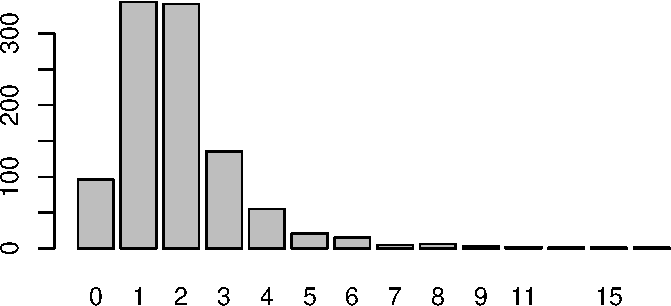
\includegraphics{./data_load_files/figure-pdf/unnamed-chunk-12-1.pdf}

}

\end{figure}

\begin{Shaded}
\begin{Highlighting}[]
\NormalTok{gg1\_core\_mDAG}\OtherTok{=}\FunctionTok{read.graph}\NormalTok{(}
  \FunctionTok{paste0}\NormalTok{(path\_exp,}\StringTok{"Global/core/core\_mDAG.graphml"}\NormalTok{), }\AttributeTok{format =} \StringTok{"graphml"}\NormalTok{)}

\NormalTok{gg1\_core\_RC}\OtherTok{=}\FunctionTok{read.graph}\NormalTok{(}
  \FunctionTok{paste0}\NormalTok{(path\_exp,                    }\StringTok{"Global/core/core\_RC.graphml"}\NormalTok{), }\AttributeTok{format =} \StringTok{"graphml"}\NormalTok{)}
\end{Highlighting}
\end{Shaded}

\begin{Shaded}
\begin{Highlighting}[]
\NormalTok{compo}\OtherTok{=}\FunctionTok{components}\NormalTok{(gg1\_mDAG,}\AttributeTok{mode =} \StringTok{"weak"}\NormalTok{)}
\FunctionTok{str}\NormalTok{(compo)}
\end{Highlighting}
\end{Shaded}

\begin{verbatim}
List of 3
 $ membership: num [1:1026] 1 1 1 1 1 1 1 1 1 1 ...
 $ csize     : num [1:167] 589 1 1 1 1 1 4 3 4 3 ...
 $ no        : int 167
\end{verbatim}

\begin{Shaded}
\begin{Highlighting}[]
\NormalTok{compo}\SpecialCharTok{$}\NormalTok{csize}
\end{Highlighting}
\end{Shaded}

\begin{verbatim}
  [1] 589   1   1   1   1   1   4   3   4   3   2   3   3   1   1   1   2   6
 [19]   3   1   3   6   1   1   1   1   1   3   1   6   2   1   1   1   2   1
 [37]   1  14   1  16   1   6   2   2   4   1   1   1   1   1   1   1   1   1
 [55]  13   1   1   1   1   2   6   5   5   2   2  10   1   1   1   2   2   1
 [73]   1   1  62   6   2   1   2   1   1   1   2   1   2  14   3   1   1   1
 [91]   1   1   1   1   1   1   3   6   1   3   1   3   2   1   1   1   2   2
[109]   3   1   1   2   5   1   1   2   3   2   1   1   2   3   4   1   1   2
[127]   1   1   2   1   1   1   1   1   3   1   2   2   1   6   1   1   1   2
[145]   1   1   1   1   1   2   7   1  15   3   1   1   1   1   2   1   3   1
[163]   1   1   1   1   2
\end{verbatim}

\begin{Shaded}
\begin{Highlighting}[]
\NormalTok{k}\OtherTok{=}\FunctionTok{which.max}\NormalTok{(compo}\SpecialCharTok{$}\NormalTok{csize}\SpecialCharTok{==}\FunctionTok{max}\NormalTok{(compo}\SpecialCharTok{$}\NormalTok{csize))}
\NormalTok{k}
\end{Highlighting}
\end{Shaded}

\begin{verbatim}
[1] 1
\end{verbatim}

\begin{Shaded}
\begin{Highlighting}[]
\FunctionTok{table}\NormalTok{(compo}\SpecialCharTok{$}\NormalTok{membership)}
\end{Highlighting}
\end{Shaded}

\begin{verbatim}

  1   2   3   4   5   6   7   8   9  10  11  12  13  14  15  16  17  18  19  20 
589   1   1   1   1   1   4   3   4   3   2   3   3   1   1   1   2   6   3   1 
 21  22  23  24  25  26  27  28  29  30  31  32  33  34  35  36  37  38  39  40 
  3   6   1   1   1   1   1   3   1   6   2   1   1   1   2   1   1  14   1  16 
 41  42  43  44  45  46  47  48  49  50  51  52  53  54  55  56  57  58  59  60 
  1   6   2   2   4   1   1   1   1   1   1   1   1   1  13   1   1   1   1   2 
 61  62  63  64  65  66  67  68  69  70  71  72  73  74  75  76  77  78  79  80 
  6   5   5   2   2  10   1   1   1   2   2   1   1   1  62   6   2   1   2   1 
 81  82  83  84  85  86  87  88  89  90  91  92  93  94  95  96  97  98  99 100 
  1   1   2   1   2  14   3   1   1   1   1   1   1   1   1   1   3   6   1   3 
101 102 103 104 105 106 107 108 109 110 111 112 113 114 115 116 117 118 119 120 
  1   3   2   1   1   1   2   2   3   1   1   2   5   1   1   2   3   2   1   1 
121 122 123 124 125 126 127 128 129 130 131 132 133 134 135 136 137 138 139 140 
  2   3   4   1   1   2   1   1   2   1   1   1   1   1   3   1   2   2   1   6 
141 142 143 144 145 146 147 148 149 150 151 152 153 154 155 156 157 158 159 160 
  1   1   1   2   1   1   1   1   1   2   7   1  15   3   1   1   1   1   2   1 
161 162 163 164 165 166 167 
  3   1   1   1   1   1   2 
\end{verbatim}

\begin{Shaded}
\begin{Highlighting}[]
\NormalTok{vertex}\OtherTok{=}\FunctionTok{which}\NormalTok{(compo}\SpecialCharTok{$}\NormalTok{membership}\SpecialCharTok{==}\NormalTok{k)}
\FunctionTok{length}\NormalTok{(vertex)}
\end{Highlighting}
\end{Shaded}

\begin{verbatim}
[1] 589
\end{verbatim}

\begin{Shaded}
\begin{Highlighting}[]
\NormalTok{vertex}
\end{Highlighting}
\end{Shaded}

\begin{verbatim}
  [1]    1    2    3    4    5    6    7    8    9   10   11   12   13   14   15
 [16]   16   17   18   19   20   21   22   23   24   25   26   27   28   29   30
 [31]   31   32   33   34   35   36   37   38   39   40   41   42   43   44   45
 [46]   46   47   48   49   50   51   52   53   54   55   56   57   58   59   60
 [61]   61   62   63   64   65   66   67   68   69   70   71   72   73   74   75
 [76]   76   77   78   79   80   81   82   83   84   85   86   87   88   89   90
 [91]   91   92   93   94   95   96   97   98   99  100  101  102  103  104  105
[106]  106  107  108  109  110  111  112  113  114  115  116  117  118  119  120
[121]  121  122  123  124  125  126  127  128  129  130  131  132  133  134  135
[136]  136  137  138  139  140  141  142  143  144  145  146  147  148  149  150
[151]  151  152  153  154  155  156  157  158  159  160  161  162  163  164  165
[166]  166  167  168  169  170  171  172  173  174  175  176  177  178  179  180
[181]  181  182  183  184  185  186  187  188  189  190  191  192  193  194  195
[196]  196  197  198  199  200  201  202  203  204  205  206  207  208  209  210
[211]  211  212  213  214  215  216  217  218  219  220  221  222  223  224  225
[226]  226  227  228  229  230  231  232  233  234  235  236  237  238  239  240
[241]  241  242  243  244  245  246  247  248  249  250  251  252  253  254  255
[256]  256  257  258  259  260  261  262  263  264  265  266  267  268  269  270
[271]  271  272  273  274  275  276  277  278  279  280  281  282  283  284  285
[286]  286  287  288  289  290  291  292  293  294  295  296  297  298  299  300
[301]  301  302  303  304  305  306  307  308  309  310  311  312  313  314  315
[316]  316  317  318  319  320  321  322  323  324  325  326  327  328  329  330
[331]  331  332  333  334  335  336  337  338  339  340  341  342  343  344  345
[346]  346  347  348  349  350  351  352  353  354  355  356  357  358  359  360
[361]  361  362  363  364  365  366  367  368  369  370  371  372  373  374  375
[376]  376  377  378  379  380  381  382  383  384  385  386  387  388  389  390
[391]  391  392  393  394  395  396  397  398  399  400  401  402  403  404  405
[406]  406  408  409  411  412  413  414  415  417  418  420  422  423  444  445
[421]  446  447  448  449  450  451  452  453  454  455  456  457  458  459  460
[436]  461  462  463  464  465  466  467  468  469  470  471  472  473  474  475
[451]  476  477  478  479  486  488  489  490  491  492  493  495  496  497  498
[466]  502  515  517  518  519  520  521  522  523  524  525  526  527  528  529
[481]  530  531  532  533  534  535  536  537  540  541  542  543  544  545  546
[496]  547  548  549  550  551  565  566  569  570  571  574  577  578  579  580
[511]  581  582  621  622  627  628  629  630  644  645  646  647  648  649  650
[526]  651  668  669  670  671  672  707  709  710  711  712  714  715  716  717
[541]  718  719  720  721  722  723  724  732  733  808  809  812  813  819  820
[556]  821  822  823  824  825  826  827  828  829  830  831  832  833  834  835
[571]  836  837  838  839  840  841  979  980  981  982  983 1003 1004 1008 1009
[586] 1010 1014 1018 1026
\end{verbatim}

\begin{Shaded}
\begin{Highlighting}[]
\FunctionTok{V}\NormalTok{(gg1\_mDAG)}
\end{Highlighting}
\end{Shaded}

\begin{verbatim}
+ 1026/1026 vertices, from b3424c4:
   [1]    1    2    3    4    5    6    7    8    9   10   11   12   13   14
  [15]   15   16   17   18   19   20   21   22   23   24   25   26   27   28
  [29]   29   30   31   32   33   34   35   36   37   38   39   40   41   42
  [43]   43   44   45   46   47   48   49   50   51   52   53   54   55   56
  [57]   57   58   59   60   61   62   63   64   65   66   67   68   69   70
  [71]   71   72   73   74   75   76   77   78   79   80   81   82   83   84
  [85]   85   86   87   88   89   90   91   92   93   94   95   96   97   98
  [99]   99  100  101  102  103  104  105  106  107  108  109  110  111  112
 [113]  113  114  115  116  117  118  119  120  121  122  123  124  125  126
 [127]  127  128  129  130  131  132  133  134  135  136  137  138  139  140
+ ... omitted several vertices
\end{verbatim}

\begin{Shaded}
\begin{Highlighting}[]
\NormalTok{CC1}\OtherTok{=}\FunctionTok{induced\_subgraph}\NormalTok{(gg1\_mDAG, }\AttributeTok{vids=}\NormalTok{vertex)}
\FunctionTok{plot}\NormalTok{(CC1)}
\end{Highlighting}
\end{Shaded}

\begin{figure}[H]

{\centering 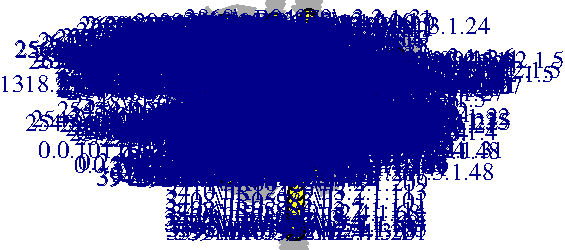
\includegraphics{./data_load_files/figure-pdf/unnamed-chunk-13-1.pdf}

}

\end{figure}

\begin{Shaded}
\begin{Highlighting}[]
\FunctionTok{summary}\NormalTok{(CC1)}
\end{Highlighting}
\end{Shaded}

\begin{verbatim}
IGRAPH b406428 D--- 589 774 -- 
+ attr: color (v/c), label (v/c), id (v/c), id (e/c)
\end{verbatim}

\bookmarksetup{startatroot}

\hypertarget{load-several-similarities-and-metadata-for-an-experiment}{%
\chapter{Load several similarities and metadata for an
experiment}\label{load-several-similarities-and-metadata-for-an-experiment}}

\begin{Shaded}
\begin{Highlighting}[]
\FunctionTok{library}\NormalTok{(tidyverse)}
\end{Highlighting}
\end{Shaded}

\begin{verbatim}
-- Attaching core tidyverse packages ------------------------ tidyverse 2.0.0 --
v dplyr     1.1.2     v readr     2.1.4
v forcats   1.0.0     v stringr   1.5.0
v ggplot2   3.4.2     v tibble    3.2.1
v lubridate 1.9.2     v tidyr     1.3.0
v purrr     1.0.1     
-- Conflicts ------------------------------------------ tidyverse_conflicts() --
x dplyr::filter() masks stats::filter()
x dplyr::lag()    masks stats::lag()
i Use the conflicted package (<http://conflicted.r-lib.org/>) to force all conflicts to become errors
\end{verbatim}

\begin{Shaded}
\begin{Highlighting}[]
\FunctionTok{library}\NormalTok{(ComplexHeatmap)}
\end{Highlighting}
\end{Shaded}

\begin{verbatim}
Loading required package: grid
========================================
ComplexHeatmap version 2.16.0
Bioconductor page: http://bioconductor.org/packages/ComplexHeatmap/
Github page: https://github.com/jokergoo/ComplexHeatmap
Documentation: http://jokergoo.github.io/ComplexHeatmap-reference

If you use it in published research, please cite either one:
- Gu, Z. Complex Heatmap Visualization. iMeta 2022.
- Gu, Z. Complex heatmaps reveal patterns and correlations in multidimensional 
    genomic data. Bioinformatics 2016.


The new InteractiveComplexHeatmap package can directly export static 
complex heatmaps into an interactive Shiny app with zero effort. Have a try!

This message can be suppressed by:
  suppressPackageStartupMessages(library(ComplexHeatmap))
========================================
\end{verbatim}

\begin{Shaded}
\begin{Highlighting}[]
\FunctionTok{library}\NormalTok{(viridis)}
\end{Highlighting}
\end{Shaded}

\begin{verbatim}
Loading required package: viridisLite
\end{verbatim}

\begin{Shaded}
\begin{Highlighting}[]
\FunctionTok{library}\NormalTok{(circlize)}
\end{Highlighting}
\end{Shaded}

\begin{verbatim}
========================================
circlize version 0.4.15
CRAN page: https://cran.r-project.org/package=circlize
Github page: https://github.com/jokergoo/circlize
Documentation: https://jokergoo.github.io/circlize_book/book/

If you use it in published research, please cite:
Gu, Z. circlize implements and enhances circular visualization
  in R. Bioinformatics 2014.

This message can be suppressed by:
  suppressPackageStartupMessages(library(circlize))
========================================
\end{verbatim}

\begin{Shaded}
\begin{Highlighting}[]
\FunctionTok{library}\NormalTok{(plotly)}
\end{Highlighting}
\end{Shaded}

\begin{verbatim}

Attaching package: 'plotly'

The following object is masked from 'package:ComplexHeatmap':

    add_heatmap

The following object is masked from 'package:ggplot2':

    last_plot

The following object is masked from 'package:stats':

    filter

The following object is masked from 'package:graphics':

    layout
\end{verbatim}

\begin{Shaded}
\begin{Highlighting}[]
\FunctionTok{library}\NormalTok{(randomcoloR)}
\CommentTok{\#library(knitr)}
\CommentTok{\#library(kableExtra)}
\FunctionTok{library}\NormalTok{(factoextra)}
\end{Highlighting}
\end{Shaded}

\begin{verbatim}
Welcome! Want to learn more? See two factoextra-related books at https://goo.gl/ve3WBa
\end{verbatim}

\begin{Shaded}
\begin{Highlighting}[]
\FunctionTok{library}\NormalTok{(RColorBrewer)}
\FunctionTok{library}\NormalTok{(kableExtra)}
\end{Highlighting}
\end{Shaded}

\begin{verbatim}

Attaching package: 'kableExtra'

The following object is masked from 'package:dplyr':

    group_rows
\end{verbatim}

\begin{Shaded}
\begin{Highlighting}[]
\NormalTok{path\_exp}\OtherTok{=}\StringTok{"data/results\_ff15c187{-}62e7{-}37c2{-}96a7{-}c824f7eab671/data/"}
\end{Highlighting}
\end{Shaded}

\hypertarget{data-analysis-whit-4-methods-distance-direct-munkrest-direct_munkrest-and-munkrest_direct}{%
\section{Data analysis whit 4 methods distance Direct, Munkrest,
Direct\_Munkrest and
Munkrest\_Direct}\label{data-analysis-whit-4-methods-distance-direct-munkrest-direct_munkrest-and-munkrest_direct}}

\hypertarget{load-several-similarities-for-mdag}{%
\section{Load several similarities for
mDag}\label{load-several-similarities-for-mdag}}

\bookmarksetup{startatroot}

\hypertarget{load-meta-data-from-experimet-all-eukariotes}{%
\chapter{Load meta data from experimet all
eukariotes}\label{load-meta-data-from-experimet-all-eukariotes}}

Meta data mDa\_Id and taxonomy sort by Kingdom,Filum,Class,mDAG\_Id

\begin{Shaded}
\begin{Highlighting}[]
\NormalTok{path\_exp}
\end{Highlighting}
\end{Shaded}

\begin{verbatim}
[1] "data/results_ff15c187-62e7-37c2-96a7-c824f7eab671/data/"
\end{verbatim}

\begin{Shaded}
\begin{Highlighting}[]
\NormalTok{Results}\OtherTok{=}\FunctionTok{read\_csv}\NormalTok{(}\FunctionTok{paste0}\NormalTok{(path\_exp,}\StringTok{"Results.csv"}\NormalTok{))}
\end{Highlighting}
\end{Shaded}

\begin{verbatim}
Rows: 884 Columns: 3997
-- Column specification --------------------------------------------------------
Delimiter: ","
chr (1924): organism, Categories, mDAG Id, Full Name, R00710(1.2.1.3), R0071...
dbl (2073): R01982(3.2.1.15), R02439(2.7.1.16), R02439_rev(2.7.1.16), R02429...

i Use `spec()` to retrieve the full column specification for this data.
i Specify the column types or set `show_col_types = FALSE` to quiet this message.
\end{verbatim}

\begin{Shaded}
\begin{Highlighting}[]
\FunctionTok{names}\NormalTok{(Results)[}\FunctionTok{c}\NormalTok{(}\DecValTok{1}\NormalTok{,}\DecValTok{3}\NormalTok{,}\DecValTok{4}\NormalTok{)]}\OtherTok{=}\FunctionTok{c}\NormalTok{(}\StringTok{"Organism"}\NormalTok{,}\StringTok{"mDAG\_Id"}\NormalTok{,}\StringTok{"Full\_Name"}\NormalTok{)}
\CommentTok{\#code=Results \%\textgreater{}\% select(Organism:mDAG\_Id)}
\NormalTok{taxo}\OtherTok{=}\NormalTok{Results }\SpecialCharTok{\%\textgreater{}\%} \FunctionTok{select}\NormalTok{(Organism}\SpecialCharTok{:}\NormalTok{Full\_Name)}
\NormalTok{index}\OtherTok{=}\FunctionTok{is.na}\NormalTok{(taxo}\SpecialCharTok{$}\NormalTok{Categories)}
\NormalTok{taxo}\OtherTok{=}\NormalTok{taxo }\SpecialCharTok{\%\textgreater{}\%} \FunctionTok{separate}\NormalTok{(Categories,}\AttributeTok{into=}\FunctionTok{c}\NormalTok{(}\StringTok{"Kingdom"}\NormalTok{,}\StringTok{"Phylum"}\NormalTok{,}\StringTok{"Class"}\NormalTok{))}
\end{Highlighting}
\end{Shaded}

\begin{verbatim}
Warning: Expected 3 pieces. Additional pieces discarded in 126 rows [27, 41, 42, 51, 62,
64, 69, 79, 80, 81, 95, 102, 109, 112, 119, 127, 132, 134, 143, 148, ...].
\end{verbatim}

\begin{verbatim}
Warning: Expected 3 pieces. Missing pieces filled with `NA` in 93 rows [11, 12, 25, 26,
43, 55, 67, 72, 78, 85, 97, 101, 108, 139, 149, 158, 165, 179, 198, 199, ...].
\end{verbatim}

\begin{Shaded}
\begin{Highlighting}[]
\NormalTok{taxo}\SpecialCharTok{$}\NormalTok{Class[index]}\OtherTok{=}\FunctionTok{paste}\NormalTok{(taxo}\SpecialCharTok{$}\NormalTok{Kingdom[index],taxo}\SpecialCharTok{$}\NormalTok{Phylum[index])}
\NormalTok{meta\_taxo}\OtherTok{=}\NormalTok{taxo }\SpecialCharTok{\%\textgreater{}\%} \FunctionTok{arrange}\NormalTok{(Kingdom,Phylum,Class)}
\CommentTok{\#order\_class=order(table(taxo$Class),decreasing = TRUE)}
\CommentTok{\#table(is.na(taxo$Class))}
\CommentTok{\#meta\_taxo= taxo \%\textgreater{}\%}
\CommentTok{\# right\_join(code,by="Organism") \%\textgreater{}\%}
\CommentTok{\#arrange(Kingdom,Phylum,Class,mDAG\_Id)}
\NormalTok{index}\OtherTok{=}\FunctionTok{which}\NormalTok{(}\FunctionTok{is.na}\NormalTok{(meta\_taxo}\SpecialCharTok{$}\NormalTok{Class))}
\NormalTok{meta\_taxo}\SpecialCharTok{$}\NormalTok{Class[index]}\OtherTok{=}\NormalTok{meta\_taxo}\SpecialCharTok{$}\NormalTok{Phylum[index]}
\end{Highlighting}
\end{Shaded}

\begin{Shaded}
\begin{Highlighting}[]
\FunctionTok{table}\NormalTok{(meta\_taxo}\SpecialCharTok{$}\NormalTok{Kingdom) }\SpecialCharTok{\%\textgreater{}\%}\NormalTok{ kable }\SpecialCharTok{\%\textgreater{}\%}
  \FunctionTok{kable\_styling}\NormalTok{(}\StringTok{"striped"}\NormalTok{, }\AttributeTok{full\_width =}\NormalTok{ F,}\AttributeTok{position=}\StringTok{"left"}\NormalTok{)}\SpecialCharTok{\%\textgreater{}\%} 
 \FunctionTok{scroll\_box}\NormalTok{(}\AttributeTok{width =} \StringTok{"400px"}\NormalTok{, }\AttributeTok{height =} \StringTok{"200px"}\NormalTok{)}
\end{Highlighting}
\end{Shaded}

\begin{tabular}{l|r}
\hline
Var1 & Freq\\
\hline
Animals & 535\\
\hline
Fungi & 154\\
\hline
Plants & 139\\
\hline
Protists & 56\\
\hline
\end{tabular}

\begin{Shaded}
\begin{Highlighting}[]
\FunctionTok{table}\NormalTok{(meta\_taxo}\SpecialCharTok{$}\NormalTok{Phylum,meta\_taxo}\SpecialCharTok{$}\NormalTok{Kingdom) }\SpecialCharTok{\%\textgreater{}\%}\NormalTok{ kable }\SpecialCharTok{\%\textgreater{}\%}
  \FunctionTok{kable\_styling}\NormalTok{(}\StringTok{"striped"}\NormalTok{, }\AttributeTok{full\_width =}\NormalTok{ F,}\AttributeTok{position=}\StringTok{"left"}\NormalTok{)}\SpecialCharTok{\%\textgreater{}\%} 
 \FunctionTok{scroll\_box}\NormalTok{(}\AttributeTok{width =} \StringTok{"500px"}\NormalTok{, }\AttributeTok{height =} \StringTok{"500px"}\NormalTok{)}
\end{Highlighting}
\end{Shaded}

\begin{tabular}{l|r|r|r|r}
\hline
  & Animals & Fungi & Plants & Protists\\
\hline
Alveolates & 0 & 0 & 0 & 25\\
\hline
Amoebozoa & 0 & 0 & 0 & 7\\
\hline
Annelids & 1 & 0 & 0 & 0\\
\hline
Arthropods & 158 & 0 & 0 & 0\\
\hline
Ascomycetes & 0 & 113 & 0 & 0\\
\hline
Basal & 0 & 0 & 2 & 0\\
\hline
Basidiomycetes & 0 & 36 & 0 & 0\\
\hline
Brachiopodas & 1 & 0 & 0 & 0\\
\hline
Cephalochordates & 2 & 0 & 0 & 0\\
\hline
Choanoflagellates & 0 & 0 & 0 & 2\\
\hline
Cnidarians & 10 & 0 & 0 & 0\\
\hline
Cryptomonads & 0 & 0 & 0 & 1\\
\hline
Echinoderms & 3 & 0 & 0 & 0\\
\hline
Eudicots & 0 & 0 & 98 & 0\\
\hline
Euglenozoa & 0 & 0 & 0 & 9\\
\hline
Ferns & 0 & 0 & 1 & 0\\
\hline
Flatworms & 4 & 0 & 0 & 0\\
\hline
Green & 0 & 0 & 11 & 0\\
\hline
Haptophyta & 0 & 0 & 0 & 1\\
\hline
Hemichordates & 1 & 0 & 0 & 0\\
\hline
Heterolobosea & 0 & 0 & 0 & 1\\
\hline
Metamonada & 0 & 0 & 0 & 2\\
\hline
Microsporidians & 0 & 5 & 0 & 0\\
\hline
Mollusks & 14 & 0 & 0 & 0\\
\hline
Monocots & 0 & 0 & 23 & 0\\
\hline
Mosses & 0 & 0 & 1 & 0\\
\hline
Nematodes & 6 & 0 & 0 & 0\\
\hline
Placozoans & 1 & 0 & 0 & 0\\
\hline
Poriferans & 1 & 0 & 0 & 0\\
\hline
Red & 0 & 0 & 3 & 0\\
\hline
Stramenopiles & 0 & 0 & 0 & 8\\
\hline
Tunicates & 2 & 0 & 0 & 0\\
\hline
Vertebrates & 331 & 0 & 0 & 0\\
\hline
\end{tabular}

\bookmarksetup{startatroot}

\hypertarget{similariries-for-method-direct}{%
\chapter{Similariries for method
Direct}\label{similariries-for-method-direct}}

In this section we will show the similarities between mDAG's using
different methods.

The experiment data set consists of 884 eurkaryotes from the animal,
plant, fungus, and protist kingdoms.

\begin{tabular}{l|r}
\hline
Kingdom & Abs. Freq.\\
\hline
Animals & 535\\
\hline
Fungi & 154\\
\hline
Plants & 139\\
\hline
Protists & 56\\
\hline
\end{tabular}

\begin{Shaded}
\begin{Highlighting}[]
\NormalTok{list\_Sim}\OtherTok{=}\FunctionTok{dir}\NormalTok{(path\_exp,}\AttributeTok{pattern=}\StringTok{"\^{}Similarities"}\NormalTok{)}
\NormalTok{list\_Sim}
\end{Highlighting}
\end{Shaded}

\begin{verbatim}
[1] "Similarities_MBB_MSAMethod.csv"               
[2] "Similarities_MBB_MunkresMethod.csv"           
[3] "Similarities_mDAG_MSAMethod.csv"              
[4] "Similarities_mDAG_MSAMethod_MunkresMethod.csv"
[5] "Similarities_mDAG_MunkresMethod.csv"          
[6] "Similarities_mDAG_MunkresMethod_MSAMethod.csv"
[7] "Similarities_mDAGOnReaction.csv"              
\end{verbatim}

\begin{Shaded}
\begin{Highlighting}[]
\NormalTok{list\_Sim\_mDAG}\OtherTok{=}\FunctionTok{dir}\NormalTok{(path\_exp,}\AttributeTok{pattern=}\StringTok{"\^{}Similarities\_mDAG"}\NormalTok{)}
\NormalTok{list\_Sim\_mDAG}
\end{Highlighting}
\end{Shaded}

\begin{verbatim}
[1] "Similarities_mDAG_MSAMethod.csv"              
[2] "Similarities_mDAG_MSAMethod_MunkresMethod.csv"
[3] "Similarities_mDAG_MunkresMethod.csv"          
[4] "Similarities_mDAG_MunkresMethod_MSAMethod.csv"
[5] "Similarities_mDAGOnReaction.csv"              
\end{verbatim}

\begin{Shaded}
\begin{Highlighting}[]
\NormalTok{Sim\_MSA\_mDAG}\OtherTok{=}\FunctionTok{read\_csv}\NormalTok{(}\FunctionTok{paste0}\NormalTok{(path\_exp,list\_Sim\_mDAG[}\DecValTok{1}\NormalTok{]))}
\end{Highlighting}
\end{Shaded}

\begin{verbatim}
New names:
Rows: 884 Columns: 885
-- Column specification
-------------------------------------------------------- Delimiter: "," chr
(1): ...1 dbl (884): 0001, 0002, 0003, 0004, 0005, 0006, 0007, 0008, 0009,
0010, 0011,...
i Use `spec()` to retrieve the full column specification for this data. i
Specify the column types or set `show_col_types = FALSE` to quiet this message.
* `` -> `...1`
\end{verbatim}

\begin{Shaded}
\begin{Highlighting}[]
\NormalTok{Sim\_MSA\_mDAG}\OtherTok{=}\FunctionTok{as.matrix}\NormalTok{(Sim\_MSA\_mDAG[,}\SpecialCharTok{{-}}\DecValTok{1}\NormalTok{])}
\FunctionTok{rownames}\NormalTok{(Sim\_MSA\_mDAG)}\OtherTok{=}\FunctionTok{colnames}\NormalTok{(Sim\_MSA\_mDAG)}
\NormalTok{Sim\_MSA\_mDAG}\OtherTok{=}\NormalTok{Sim\_MSA\_mDAG[meta\_taxo}\SpecialCharTok{$}\NormalTok{mDAG\_Id,meta\_taxo}\SpecialCharTok{$}\NormalTok{mDAG\_Id]}
\end{Highlighting}
\end{Shaded}

\begin{Shaded}
\begin{Highlighting}[]
\NormalTok{Sim\_MSA\_Mun\_mDAG}\OtherTok{=}\FunctionTok{read\_csv}\NormalTok{(}\FunctionTok{paste0}\NormalTok{(path\_exp,list\_Sim\_mDAG[}\DecValTok{2}\NormalTok{]))}
\end{Highlighting}
\end{Shaded}

\begin{verbatim}
New names:
Rows: 884 Columns: 885
-- Column specification
-------------------------------------------------------- Delimiter: "," chr
(1): ...1 dbl (884): 0001, 0002, 0003, 0004, 0005, 0006, 0007, 0008, 0009,
0010, 0011,...
i Use `spec()` to retrieve the full column specification for this data. i
Specify the column types or set `show_col_types = FALSE` to quiet this message.
* `` -> `...1`
\end{verbatim}

\begin{Shaded}
\begin{Highlighting}[]
\NormalTok{Sim\_MSA\_Mun\_mDAG}\OtherTok{=}\FunctionTok{as.matrix}\NormalTok{(Sim\_MSA\_Mun\_mDAG[,}\SpecialCharTok{{-}}\DecValTok{1}\NormalTok{])}
\FunctionTok{rownames}\NormalTok{(Sim\_MSA\_Mun\_mDAG)}\OtherTok{=}\FunctionTok{colnames}\NormalTok{(Sim\_MSA\_Mun\_mDAG)}
\NormalTok{Sim\_MSA\_Mun\_mDAG}\OtherTok{=}\NormalTok{Sim\_MSA\_Mun\_mDAG[meta\_taxo}\SpecialCharTok{$}\NormalTok{mDAG\_Id,meta\_taxo}\SpecialCharTok{$}\NormalTok{mDAG\_Id]}
\end{Highlighting}
\end{Shaded}

\begin{Shaded}
\begin{Highlighting}[]
\NormalTok{Sim\_Mun\_mDAG}\OtherTok{=}\FunctionTok{read\_csv}\NormalTok{(}\FunctionTok{paste0}\NormalTok{(path\_exp,list\_Sim\_mDAG[}\DecValTok{3}\NormalTok{]))}
\end{Highlighting}
\end{Shaded}

\begin{verbatim}
New names:
Rows: 884 Columns: 885
-- Column specification
-------------------------------------------------------- Delimiter: "," chr
(1): ...1 dbl (884): 0001, 0002, 0003, 0004, 0005, 0006, 0007, 0008, 0009,
0010, 0011,...
i Use `spec()` to retrieve the full column specification for this data. i
Specify the column types or set `show_col_types = FALSE` to quiet this message.
* `` -> `...1`
\end{verbatim}

\begin{Shaded}
\begin{Highlighting}[]
\NormalTok{Sim\_Mun\_mDAG}\OtherTok{=}\FunctionTok{as.matrix}\NormalTok{(Sim\_Mun\_mDAG[,}\SpecialCharTok{{-}}\DecValTok{1}\NormalTok{])}
\FunctionTok{rownames}\NormalTok{(Sim\_Mun\_mDAG)}\OtherTok{=}\FunctionTok{colnames}\NormalTok{(Sim\_Mun\_mDAG)}
\NormalTok{Sim\_MSA\_mDAG}\OtherTok{=}\NormalTok{Sim\_MSA\_mDAG[meta\_taxo}\SpecialCharTok{$}\NormalTok{mDAG\_Id,meta\_taxo}\SpecialCharTok{$}\NormalTok{mDAG\_Id]}
\end{Highlighting}
\end{Shaded}

\begin{Shaded}
\begin{Highlighting}[]
\NormalTok{Sim\_Mun\_MSA\_mDAG}\OtherTok{=}\FunctionTok{read\_csv}\NormalTok{(}\FunctionTok{paste0}\NormalTok{(path\_exp,list\_Sim\_mDAG[}\DecValTok{4}\NormalTok{]))}
\end{Highlighting}
\end{Shaded}

\begin{verbatim}
New names:
Rows: 884 Columns: 885
-- Column specification
-------------------------------------------------------- Delimiter: "," chr
(1): ...1 dbl (884): 0001, 0002, 0003, 0004, 0005, 0006, 0007, 0008, 0009,
0010, 0011,...
i Use `spec()` to retrieve the full column specification for this data. i
Specify the column types or set `show_col_types = FALSE` to quiet this message.
* `` -> `...1`
\end{verbatim}

\begin{Shaded}
\begin{Highlighting}[]
\NormalTok{Sim\_Mun\_MSA\_mDAG}\OtherTok{=}\FunctionTok{as.matrix}\NormalTok{(Sim\_Mun\_MSA\_mDAG[,}\SpecialCharTok{{-}}\DecValTok{1}\NormalTok{])}
\FunctionTok{rownames}\NormalTok{(Sim\_Mun\_MSA\_mDAG)}\OtherTok{=}\FunctionTok{colnames}\NormalTok{(Sim\_Mun\_MSA\_mDAG)}
\NormalTok{Sim\_Mun\_MSA\_mDAG}\OtherTok{=}\NormalTok{Sim\_Mun\_MSA\_mDAG[meta\_taxo}\SpecialCharTok{$}\NormalTok{mDAG\_Id,meta\_taxo}\SpecialCharTok{$}\NormalTok{mDAG\_Id]}
\end{Highlighting}
\end{Shaded}

\hypertarget{heatmaps}{%
\section{Heatmaps}\label{heatmaps}}

\begin{verbatim}
dis_DirectedMethod<-read_csv(paste0(path_exp,
                                    "Similarities_MBB_MSAMethod.csv"))
names(dis_DirectedMethod)[1]="mDAG_Id"
dis_DirectedMethod[,-1]=sqrt(1-dis_DirectedMethod[,-1])
dis_DirectedMethod_meta =dis_DirectedMethod %>% right_join(select(meta_taxo,mDAG_Id,Kingdom,Filum,Class),by="mDAG_Id") %>%
  arrange(Kingdom,Filum,Class)


ID=dis_DirectedMethod_meta$mDAG_Id
dis_DirectedMethod=  dis_DirectedMethod_meta %>% 
  select(-Kingdom) %>% 
  relocate(mDAG_Id,ID) %>%
  select(2:570) %>%
  as.matrix()
#dis_dir=as.matrix(sqrt(2*(1-sim0[,c(2:570)]^2)))
dimnames(dis_DirectedMethod) = list(ID,ID)
\end{verbatim}

\hypertarget{heatmap-similarity-msa-method}{%
\section{Heatmap Similarity MSA
method}\label{heatmap-similarity-msa-method}}

\begin{Shaded}
\begin{Highlighting}[]
\NormalTok{dff}\OtherTok{\textless{}{-}}\NormalTok{meta\_taxo }\SpecialCharTok{\%\textgreater{}\%} \FunctionTok{select}\NormalTok{(Kingdom)  }\SpecialCharTok{\%\textgreater{}\%} \FunctionTok{as.data.frame}\NormalTok{()}
\CommentTok{\#str(dff)}

\NormalTok{colores }\OtherTok{\textless{}{-}} \FunctionTok{list}\NormalTok{(}\AttributeTok{Kingdom=} \FunctionTok{c}\NormalTok{(}\StringTok{"Animals"}\OtherTok{=}\StringTok{"purple"}\NormalTok{,}\StringTok{"Plants"}\OtherTok{=}\StringTok{"green"}\NormalTok{,}\StringTok{"Fungi"}\OtherTok{=}\StringTok{"yellow"}\NormalTok{,}\StringTok{"Protists"}\OtherTok{=}\StringTok{"coral"}\NormalTok{))}

\NormalTok{anotacion }\OtherTok{\textless{}{-}} \FunctionTok{HeatmapAnnotation}\NormalTok{(}\AttributeTok{df=}\NormalTok{dff, }\AttributeTok{col =}\NormalTok{ colores)}

\NormalTok{S}\OtherTok{=}\NormalTok{Sim\_MSA\_mDAG}
\NormalTok{a}\OtherTok{\textless{}{-}} \FunctionTok{Heatmap}\NormalTok{(}\AttributeTok{matrix =}\NormalTok{ Sim\_MSA\_mDAG, }
                          \AttributeTok{column\_title=}\StringTok{"Similarity mDag MSA Method}\SpecialCharTok{\textbackslash{}n}\StringTok{  Eukariotas by Kingdom"}\NormalTok{,}
            \AttributeTok{name =} \StringTok{"Kingdom"}\NormalTok{,}
            \AttributeTok{heatmap\_legend\_param =} \FunctionTok{list}\NormalTok{(}
    \AttributeTok{at =} \FunctionTok{c}\NormalTok{(}\FloatTok{0.4}\NormalTok{,}\FloatTok{0.5}\NormalTok{,}\FloatTok{0.6}\NormalTok{,}\FloatTok{0.7}\NormalTok{,}\FloatTok{0.8}\NormalTok{,}\FloatTok{0.9}\NormalTok{,}\DecValTok{1}\NormalTok{)),}
        \AttributeTok{col=}\FunctionTok{rev}\NormalTok{(}\FunctionTok{viridis}\NormalTok{(}\DecValTok{256}\NormalTok{)),}
        \AttributeTok{cluster\_rows =} \ConstantTok{FALSE}\NormalTok{,}
        \AttributeTok{cluster\_columns =} \ConstantTok{FALSE}\NormalTok{,}
        \AttributeTok{top\_annotation =}\NormalTok{ anotacion,}
        \AttributeTok{show\_column\_names =} \ConstantTok{FALSE}\NormalTok{, }
        \AttributeTok{show\_row\_names =} \ConstantTok{FALSE}\NormalTok{,}
        \AttributeTok{left\_annotation =} \FunctionTok{rowAnnotation}\NormalTok{(}\AttributeTok{df =}\NormalTok{ dff, }\AttributeTok{col =}\NormalTok{ colores,}\AttributeTok{show\_annotation\_name=}\ConstantTok{FALSE}\NormalTok{))}
  
\FunctionTok{draw}\NormalTok{(a, }\AttributeTok{merge\_legend =} \ConstantTok{TRUE}\NormalTok{)}
\end{Highlighting}
\end{Shaded}

\begin{figure}[H]

{\centering 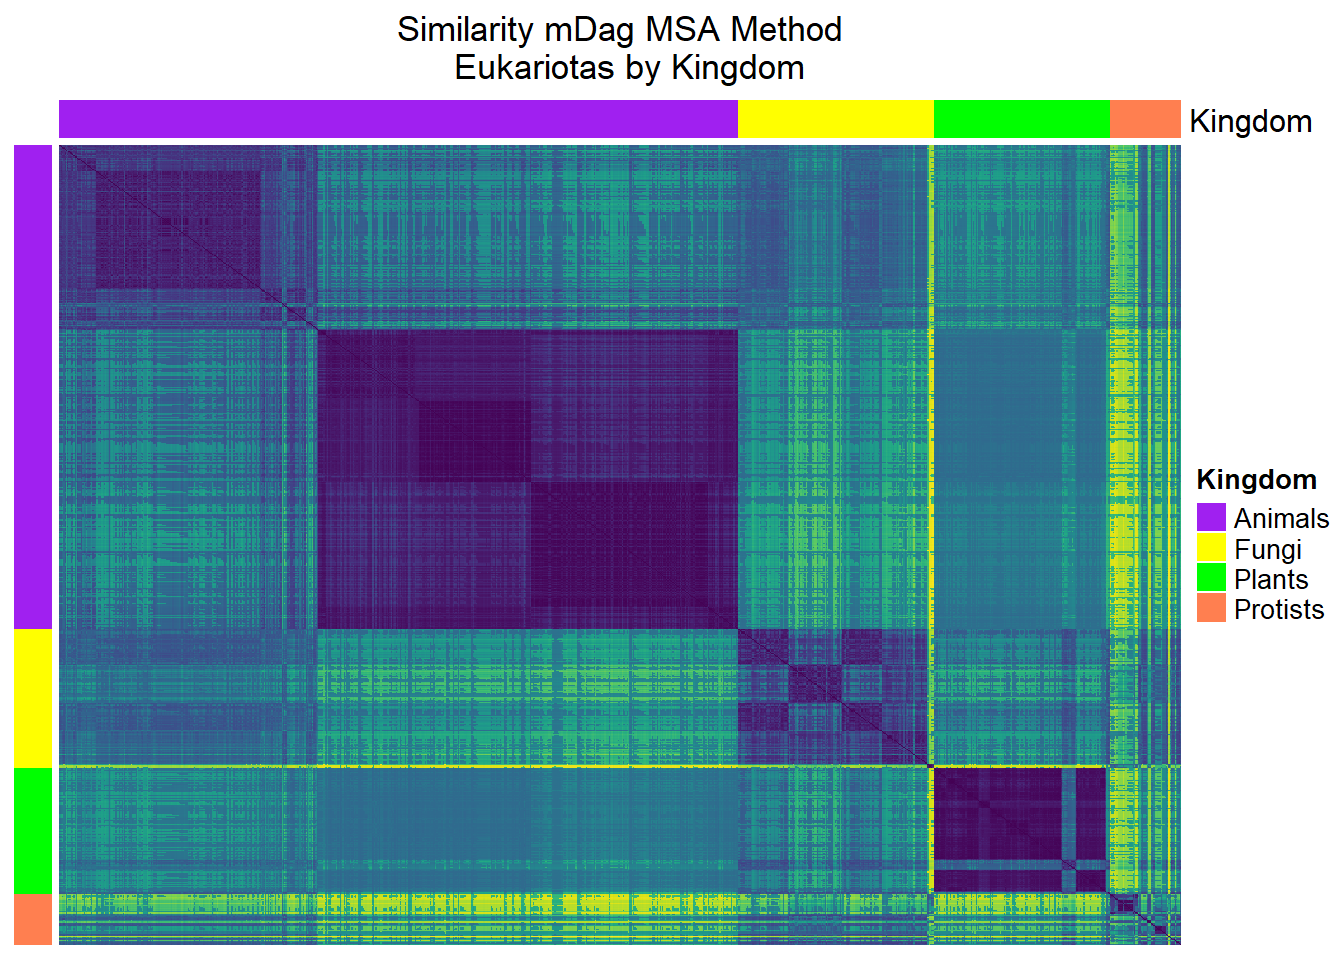
\includegraphics{./data_medag_20230321_long_report_files/figure-pdf/unnamed-chunk-10-1.pdf}

}

\end{figure}

\begin{Shaded}
\begin{Highlighting}[]
\NormalTok{meta\_animals}\OtherTok{=}\NormalTok{ meta\_taxo }\SpecialCharTok{\%\textgreater{}\%} \FunctionTok{filter}\NormalTok{(Kingdom}\SpecialCharTok{==}\StringTok{"Animals"}\NormalTok{)}
\NormalTok{nombres}\OtherTok{=}\FunctionTok{unique}\NormalTok{(meta\_animals}\SpecialCharTok{$}\NormalTok{Phylum)}
\NormalTok{aux\_order}\OtherTok{=}\FunctionTok{table}\NormalTok{(meta\_animals}\SpecialCharTok{$}\NormalTok{Phylum)}
\NormalTok{dff}\OtherTok{\textless{}{-}}\NormalTok{meta\_taxo }\SpecialCharTok{\%\textgreater{}\%} \FunctionTok{filter}\NormalTok{(Kingdom}\SpecialCharTok{==}\StringTok{"Animals"}\NormalTok{) }\SpecialCharTok{\%\textgreater{}\%} \FunctionTok{select}\NormalTok{(Class) }\SpecialCharTok{\%\textgreater{}\%} \FunctionTok{as.data.frame}\NormalTok{()}
\CommentTok{\#str(dff)}
\NormalTok{nombres}\OtherTok{=}\FunctionTok{unique}\NormalTok{(dff}\SpecialCharTok{$}\NormalTok{Class)}
\NormalTok{col}\OtherTok{=}\FunctionTok{rainbow}\NormalTok{(}\FunctionTok{length}\NormalTok{(nombres))}
\NormalTok{colores}\OtherTok{=}\FunctionTok{list}\NormalTok{(}\AttributeTok{Class=}\NormalTok{col)}
\FunctionTok{names}\NormalTok{(colores}\SpecialCharTok{$}\NormalTok{Class)}\OtherTok{=}\NormalTok{nombres}
\CommentTok{\#paste0(paste0(\textquotesingle{}"\textquotesingle{},nombres,\textquotesingle{}"="\textquotesingle{},col,\textquotesingle{}"\textquotesingle{}),collapse=",")}
\CommentTok{\# colores \textless{}{-} list(Class=c(}
\CommentTok{\# "Amphibians"="\#FF0000","Annelids"="\#FF4900",}
\CommentTok{\# "Cartilaginous"="\#FF9200","Cephalochordates"="\#FFDB00",}
\CommentTok{\# "Chelicerates"="\#DBFF00","Cnidarians"="\#92FF00",}
\CommentTok{\# "Crustaceans"="\#49FF00","Echinoderms"="\#00FF00",}
\CommentTok{\# "Fishes"="\#00FF49","Flatworms"="\#00FF92",}
\CommentTok{\# "Hemichordates"="\#00FFDB","Insects"="\#00DBFF",}
\CommentTok{\# "Mammals"="\#0092FF","Mollusks"="\#0049FF",}
\CommentTok{\# "Nematodes"="\#0000FF","Placozoans"="\#4900FF",}
\CommentTok{\# "Poriferans"="\#9200FF",}
\CommentTok{\# "Reptiles"="\#DB00FF",}
\CommentTok{\# "Tunicates"="\#FF00DB",}
\CommentTok{\# "Mammals"="\#FF0092",}
\CommentTok{\# "Reptiles"="\#FF0049"))}
\CommentTok{\# aux=names(colores$Class)}
\CommentTok{\# colores$Class=as.character(palette.colors(n=21,palette="Polychrome 36"))}
\CommentTok{\# attr(colores$Class,"names")=aux}


\NormalTok{anotacion }\OtherTok{\textless{}{-}} \FunctionTok{HeatmapAnnotation}\NormalTok{(}\AttributeTok{df=}\NormalTok{dff, }\AttributeTok{col =}\NormalTok{ colores)}


\NormalTok{a2}\OtherTok{\textless{}{-}} \FunctionTok{Heatmap}\NormalTok{(}\AttributeTok{matrix =}\NormalTok{ S[}\DecValTok{1}\SpecialCharTok{:}\DecValTok{535}\NormalTok{,}\DecValTok{1}\SpecialCharTok{:}\DecValTok{535}\NormalTok{], }
              \AttributeTok{column\_title=}\StringTok{"Distance mDag Direct Method}\SpecialCharTok{\textbackslash{}n}\StringTok{  Animals by Class"}\NormalTok{,}
            \AttributeTok{name =} \StringTok{"Class"}\NormalTok{, }
            \AttributeTok{heatmap\_legend\_param =} \FunctionTok{list}\NormalTok{(}
    \AttributeTok{at =} \FunctionTok{seq}\NormalTok{(}\DecValTok{0}\NormalTok{,}\FloatTok{1.5}\NormalTok{,}\AttributeTok{by=}\FloatTok{0.1}\NormalTok{)),}
        \AttributeTok{col=}\FunctionTok{rev}\NormalTok{(}\FunctionTok{viridis}\NormalTok{(}\DecValTok{256}\NormalTok{)),}
        \AttributeTok{cluster\_rows =} \ConstantTok{FALSE}\NormalTok{,}
        \AttributeTok{cluster\_columns =} \ConstantTok{FALSE}\NormalTok{,}
        \AttributeTok{top\_annotation =}\NormalTok{ anotacion,}
        \AttributeTok{show\_column\_names =} \ConstantTok{FALSE}\NormalTok{, }
        \AttributeTok{show\_row\_names =} \ConstantTok{FALSE}\NormalTok{,}
        \AttributeTok{left\_annotation =} \FunctionTok{rowAnnotation}\NormalTok{(}\AttributeTok{df =}\NormalTok{ dff, }\AttributeTok{col =}\NormalTok{ colores,}\AttributeTok{show\_annotation\_name=}\ConstantTok{FALSE}\NormalTok{))}
  
\FunctionTok{draw}\NormalTok{(a2, }\AttributeTok{merge\_legend =} \ConstantTok{TRUE}\NormalTok{)}
\end{Highlighting}
\end{Shaded}

\begin{figure}[H]

{\centering 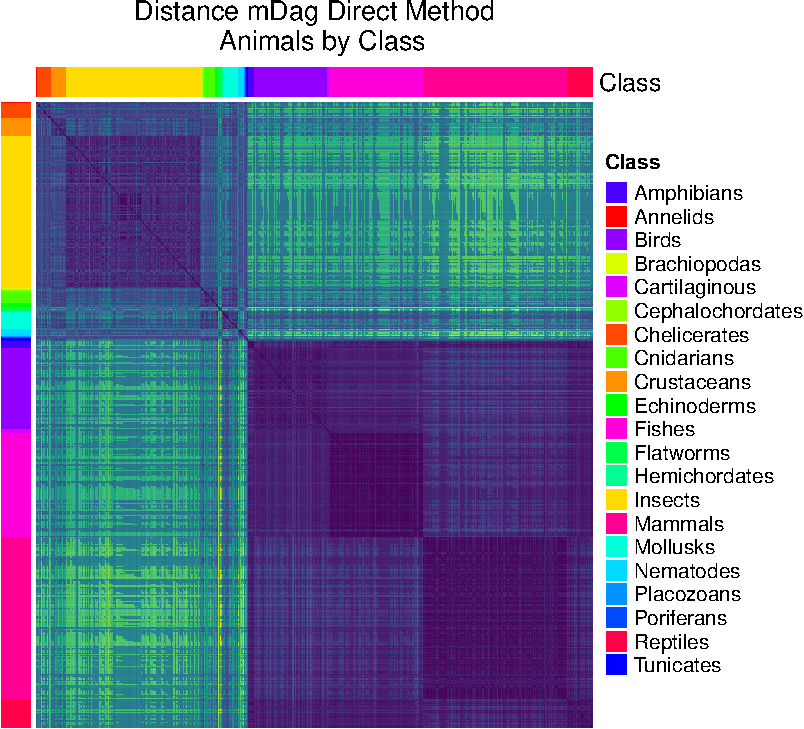
\includegraphics{./data_medag_20230321_long_report_files/figure-pdf/unnamed-chunk-11-1.pdf}

}

\end{figure}

\hypertarget{mds-multidimensional-scaling}{%
\section{MDS (Multidimensional
Scaling)}\label{mds-multidimensional-scaling}}

\begin{Shaded}
\begin{Highlighting}[]
\DocumentationTok{\#\# Metric multidimensional scaling (mMDS)}
\NormalTok{mds7 }\OtherTok{\textless{}{-}} \FunctionTok{cmdscale}\NormalTok{(}\FunctionTok{sqrt}\NormalTok{(}\DecValTok{1}\SpecialCharTok{{-}}\NormalTok{Sim\_MSA\_mDAG}\SpecialCharTok{\^{}}\DecValTok{2}\NormalTok{),}\AttributeTok{k=}\DecValTok{7}\NormalTok{,}\AttributeTok{eig=}\ConstantTok{TRUE}\NormalTok{)}
\CommentTok{\#pairs(mds7$points[,1:4])}
\NormalTok{mds7}\SpecialCharTok{$}\NormalTok{GOF}
\end{Highlighting}
\end{Shaded}

\begin{verbatim}
[1] 0.4406568 0.5541042
\end{verbatim}

\begin{Shaded}
\begin{Highlighting}[]
\NormalTok{mds }\OtherTok{\textless{}{-}}\NormalTok{ mds7}\SpecialCharTok{$}\NormalTok{points }\SpecialCharTok{\%\textgreater{}\%}  \FunctionTok{as\_tibble}\NormalTok{()}
\end{Highlighting}
\end{Shaded}

\begin{verbatim}
Warning: The `x` argument of `as_tibble.matrix()` must have unique column names if
`.name_repair` is omitted as of tibble 2.0.0.
i Using compatibility `.name_repair`.
\end{verbatim}

\begin{Shaded}
\begin{Highlighting}[]
\FunctionTok{colnames}\NormalTok{(mds) }\OtherTok{\textless{}{-}}\FunctionTok{paste0}\NormalTok{(}\StringTok{"Dim."}\NormalTok{,}\DecValTok{1}\SpecialCharTok{:}\FunctionTok{dim}\NormalTok{(mds7}\SpecialCharTok{$}\NormalTok{points)[}\DecValTok{2}\NormalTok{])}

\FunctionTok{library}\NormalTok{(GGally)}
\end{Highlighting}
\end{Shaded}

\begin{verbatim}
Registered S3 method overwritten by 'GGally':
  method from   
  +.gg   ggplot2
\end{verbatim}

\begin{Shaded}
\begin{Highlighting}[]
\FunctionTok{ggpairs}\NormalTok{(}\FunctionTok{as\_tibble}\NormalTok{(mds7}\SpecialCharTok{$}\NormalTok{points),}\AttributeTok{columns=}\DecValTok{1}\SpecialCharTok{:}\DecValTok{4}\NormalTok{,}\FunctionTok{aes}\NormalTok{(}\AttributeTok{color=}\NormalTok{meta\_taxo}\SpecialCharTok{$}\NormalTok{Kingdom,}\AttributeTok{alpha=}\FloatTok{0.5}\NormalTok{),}\AttributeTok{upper=}\FunctionTok{list}\NormalTok{(}\AttributeTok{continuous=}\StringTok{"points"}\NormalTok{)) }
\end{Highlighting}
\end{Shaded}

\begin{figure}[H]

{\centering 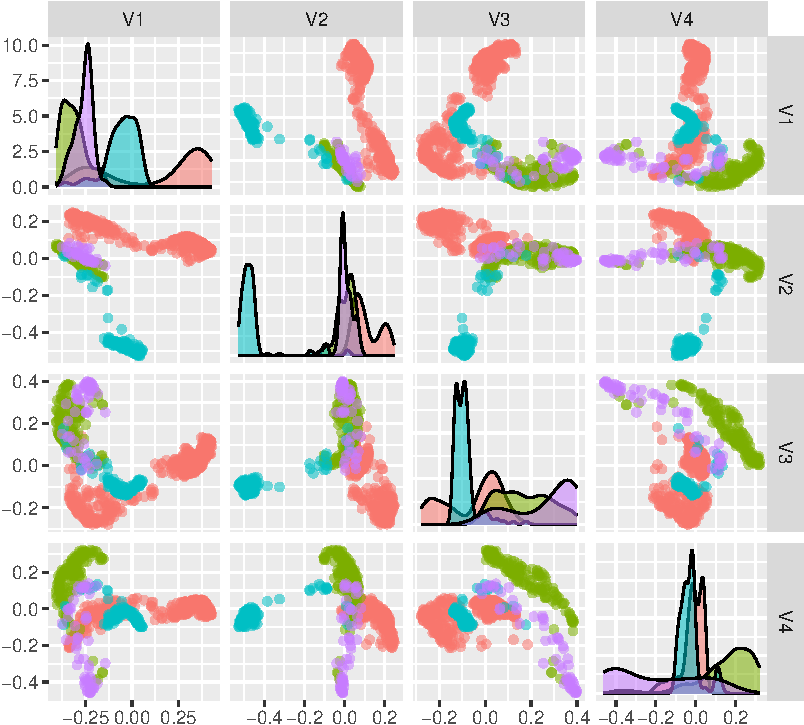
\includegraphics{./data_medag_20230321_long_report_files/figure-pdf/unnamed-chunk-12-1.pdf}

}

\end{figure}

\begin{Shaded}
\begin{Highlighting}[]
\NormalTok{mds }\OtherTok{\textless{}{-}}\NormalTok{ mds }\SpecialCharTok{\%\textgreater{}\%}
  \FunctionTok{mutate}\NormalTok{(}\AttributeTok{groups =}\FunctionTok{as.factor}\NormalTok{(meta\_taxo}\SpecialCharTok{$}\NormalTok{Kingdom))}


\CommentTok{\#,text= \textasciitilde{}paste("Age:", groups, \textquotesingle{}\textless{}br\textgreater{}Name:\textquotesingle{})}
\FunctionTok{length}\NormalTok{(}\FunctionTok{unique}\NormalTok{(meta\_taxo}\SpecialCharTok{$}\NormalTok{Phylum))}
\end{Highlighting}
\end{Shaded}

\begin{verbatim}
[1] 33
\end{verbatim}

\begin{Shaded}
\begin{Highlighting}[]
\CommentTok{\#col\_mds=c("purple","green","yellow","coral")}
\NormalTok{col\_mds}\OtherTok{=}\FunctionTok{rainbow}\NormalTok{(}\DecValTok{33}\NormalTok{)}
\CommentTok{\#mcol\_mds=bremer.pal(7,"Greens")}

\NormalTok{fig }\OtherTok{\textless{}{-}} 
\FunctionTok{plot\_ly}\NormalTok{(}
\NormalTok{  mds, }\AttributeTok{x =} \SpecialCharTok{\textasciitilde{}}\NormalTok{Dim}\FloatTok{.1}\NormalTok{, }\AttributeTok{y =} \SpecialCharTok{\textasciitilde{}}\NormalTok{Dim}\FloatTok{.2}\NormalTok{,}
  \AttributeTok{color =} \SpecialCharTok{\textasciitilde{}}\NormalTok{groups, }
  \AttributeTok{colors=}\NormalTok{ col\_mds,}
  \AttributeTok{type=}\StringTok{"scatter"}\NormalTok{,}
  \AttributeTok{mode=}\StringTok{"markers"}\NormalTok{) }\SpecialCharTok{\%\textgreater{}\%}
  \FunctionTok{layout}\NormalTok{(}
    \AttributeTok{xaxis =} \FunctionTok{list}\NormalTok{(}\AttributeTok{autorange=}\DecValTok{2}\NormalTok{,}
      \AttributeTok{range=}\FunctionTok{c}\NormalTok{(}\SpecialCharTok{{-}}\FloatTok{0.8}\NormalTok{,}\FloatTok{0.8}\NormalTok{)), }\AttributeTok{yaxis =} \FunctionTok{list}\NormalTok{(}\AttributeTok{autorange=}\DecValTok{2}\NormalTok{,}
      \AttributeTok{range=}\FunctionTok{c}\NormalTok{(}\SpecialCharTok{{-}}\FloatTok{0.8}\NormalTok{,}\FloatTok{0.8}\NormalTok{)))}


\CommentTok{\#fig}
\end{Highlighting}
\end{Shaded}

\bookmarksetup{startatroot}

\hypertarget{hierarchical-cluster}{%
\chapter{Hierarchical cluster}\label{hierarchical-cluster}}

\begin{Shaded}
\begin{Highlighting}[]
\FunctionTok{library}\NormalTok{(dendextend)}
\end{Highlighting}
\end{Shaded}

\begin{verbatim}

---------------------
Welcome to dendextend version 1.17.1
Type citation('dendextend') for how to cite the package.

Type browseVignettes(package = 'dendextend') for the package vignette.
The github page is: https://github.com/talgalili/dendextend/

Suggestions and bug-reports can be submitted at: https://github.com/talgalili/dendextend/issues
You may ask questions at stackoverflow, use the r and dendextend tags: 
     https://stackoverflow.com/questions/tagged/dendextend

    To suppress this message use:  suppressPackageStartupMessages(library(dendextend))
---------------------
\end{verbatim}

\begin{verbatim}

Attaching package: 'dendextend'
\end{verbatim}

\begin{verbatim}
The following object is masked from 'package:stats':

    cutree
\end{verbatim}

\begin{Shaded}
\begin{Highlighting}[]
\NormalTok{D}\OtherTok{=}\FunctionTok{as.dist}\NormalTok{(}\FunctionTok{sqrt}\NormalTok{(}\DecValTok{1}\SpecialCharTok{{-}}\NormalTok{Sim\_MSA\_mDAG}\SpecialCharTok{\^{}}\DecValTok{2}\NormalTok{))}
\NormalTok{hc}\OtherTok{=}\FunctionTok{hclust}\NormalTok{(}\FunctionTok{as.dist}\NormalTok{(D),}\AttributeTok{method =}\StringTok{"ward.D"}\NormalTok{)}
\FunctionTok{ggplot}\NormalTok{(}\FunctionTok{as.ggdend}\NormalTok{(}\FunctionTok{as.dendrogram}\NormalTok{(hc)))}
\end{Highlighting}
\end{Shaded}

\begin{figure}[H]

{\centering 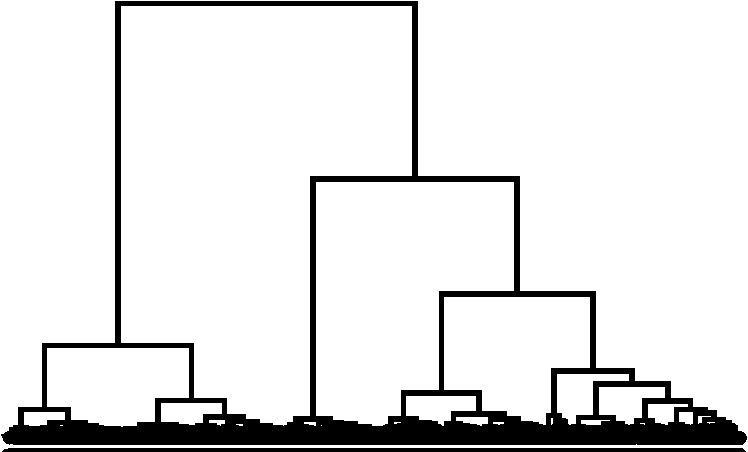
\includegraphics{./data_medag_20230321_long_report_files/figure-pdf/unnamed-chunk-13-1.pdf}

}

\end{figure}

\begin{Shaded}
\begin{Highlighting}[]
\NormalTok{clust4}\OtherTok{=}\FunctionTok{cutree}\NormalTok{(hc,}\DecValTok{4}\NormalTok{)}
\FunctionTok{table}\NormalTok{(clust4,meta\_taxo}\SpecialCharTok{$}\NormalTok{Kingdom)}
\end{Highlighting}
\end{Shaded}

\begin{verbatim}
      
clust4 Animals Fungi Plants Protists
     1     195     0      0        0
     2       9   154     14       56
     3     331     0      0        0
     4       0     0    125        0
\end{verbatim}

\hypertarget{heatmap-similarity-mun_msa-method}{%
\section{Heatmap Similarity Mun\_MSA
method}\label{heatmap-similarity-mun_msa-method}}

\begin{Shaded}
\begin{Highlighting}[]
\NormalTok{dff}\OtherTok{\textless{}{-}}\NormalTok{meta\_taxo }\SpecialCharTok{\%\textgreater{}\%} \FunctionTok{select}\NormalTok{(Kingdom)  }\SpecialCharTok{\%\textgreater{}\%} \FunctionTok{as.data.frame}\NormalTok{()}
\CommentTok{\#str(dff)}

\NormalTok{colores }\OtherTok{\textless{}{-}} \FunctionTok{list}\NormalTok{(}\AttributeTok{Kingdom=} \FunctionTok{c}\NormalTok{(}\StringTok{"Animals"}\OtherTok{=}\StringTok{"purple"}\NormalTok{,}\StringTok{"Plants"}\OtherTok{=}\StringTok{"green"}\NormalTok{,}\StringTok{"Fungi"}\OtherTok{=}\StringTok{"yellow"}\NormalTok{,}\StringTok{"Protists"}\OtherTok{=}\StringTok{"coral"}\NormalTok{))}

\NormalTok{anotacion }\OtherTok{\textless{}{-}} \FunctionTok{HeatmapAnnotation}\NormalTok{(}\AttributeTok{df=}\NormalTok{dff, }\AttributeTok{col =}\NormalTok{ colores)}

\NormalTok{S}\OtherTok{=}\NormalTok{Sim\_Mun\_MSA\_mDAG}
\NormalTok{a}\OtherTok{\textless{}{-}} \FunctionTok{Heatmap}\NormalTok{(}\AttributeTok{matrix =}\NormalTok{ Sim\_Mun\_MSA\_mDAG, }
                          \AttributeTok{column\_title=}\StringTok{"Similarity mDag Mun{-}MSA Method}\SpecialCharTok{\textbackslash{}n}\StringTok{  Eukariotas by Kingdom"}\NormalTok{,}
            \AttributeTok{name =} \StringTok{"Kingdom"}\NormalTok{,}
            \AttributeTok{heatmap\_legend\_param =} \FunctionTok{list}\NormalTok{(}
    \AttributeTok{at =} \FunctionTok{c}\NormalTok{(}\FloatTok{0.4}\NormalTok{,}\FloatTok{0.5}\NormalTok{,}\FloatTok{0.6}\NormalTok{,}\FloatTok{0.7}\NormalTok{,}\FloatTok{0.8}\NormalTok{,}\FloatTok{0.9}\NormalTok{,}\DecValTok{1}\NormalTok{)),}
        \AttributeTok{col=}\FunctionTok{rev}\NormalTok{(}\FunctionTok{viridis}\NormalTok{(}\DecValTok{256}\NormalTok{)),}
        \AttributeTok{cluster\_rows =} \ConstantTok{FALSE}\NormalTok{,}
        \AttributeTok{cluster\_columns =} \ConstantTok{FALSE}\NormalTok{,}
        \AttributeTok{top\_annotation =}\NormalTok{ anotacion,}
        \AttributeTok{show\_column\_names =} \ConstantTok{FALSE}\NormalTok{, }
        \AttributeTok{show\_row\_names =} \ConstantTok{FALSE}\NormalTok{,}
        \AttributeTok{left\_annotation =} \FunctionTok{rowAnnotation}\NormalTok{(}\AttributeTok{df =}\NormalTok{ dff, }\AttributeTok{col =}\NormalTok{ colores,}\AttributeTok{show\_annotation\_name=}\ConstantTok{FALSE}\NormalTok{))}
  
\FunctionTok{draw}\NormalTok{(a, }\AttributeTok{merge\_legend =} \ConstantTok{TRUE}\NormalTok{)}
\end{Highlighting}
\end{Shaded}

\begin{figure}[H]

{\centering 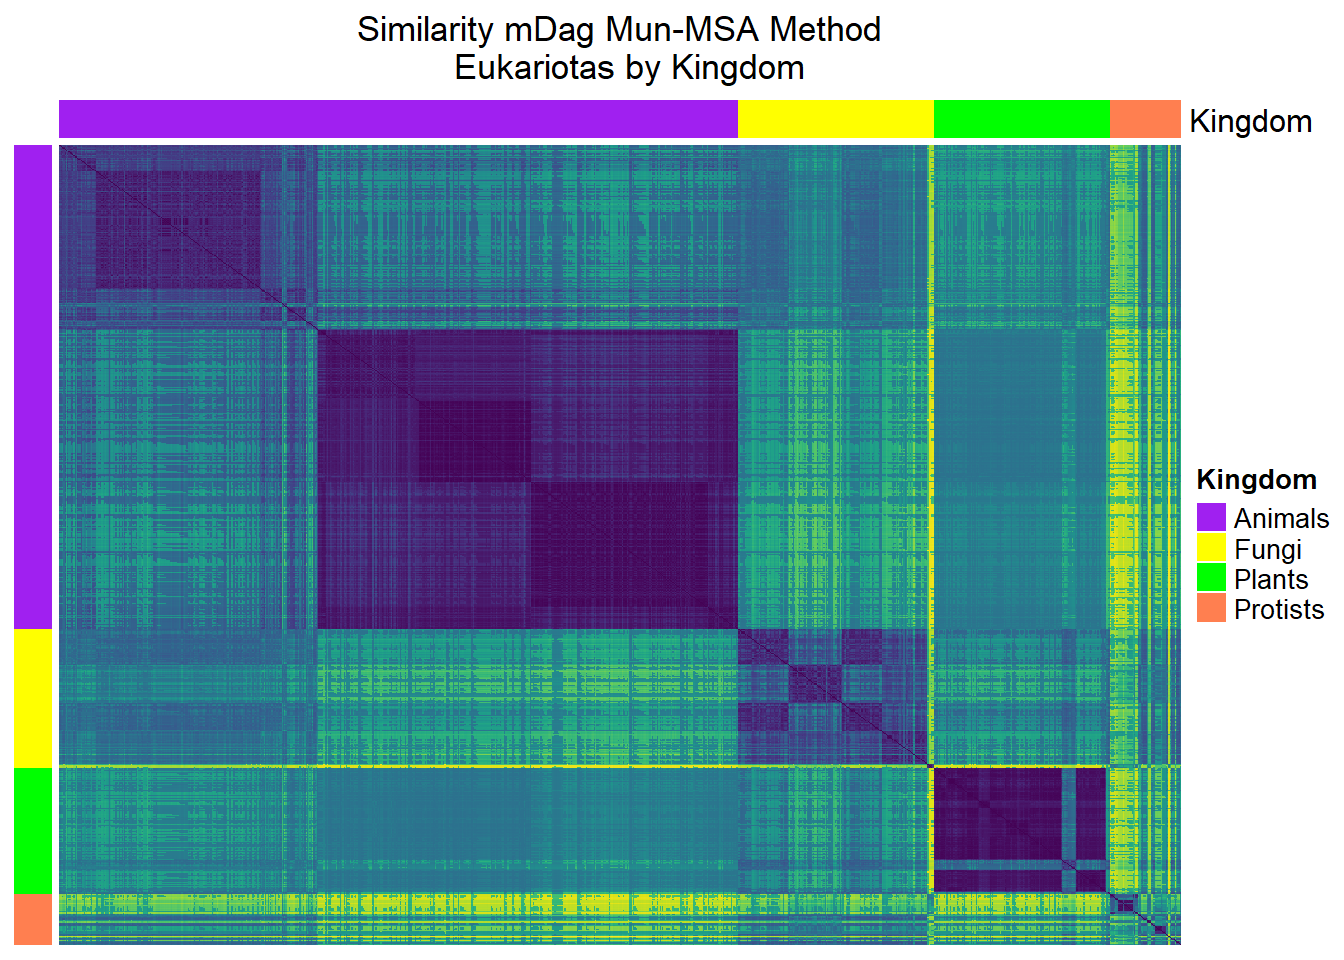
\includegraphics{./data_medag_20230321_long_report_files/figure-pdf/unnamed-chunk-15-1.pdf}

}

\end{figure}

\begin{Shaded}
\begin{Highlighting}[]
\NormalTok{meta\_animals}\OtherTok{=}\NormalTok{ meta\_taxo }\SpecialCharTok{\%\textgreater{}\%} \FunctionTok{filter}\NormalTok{(Kingdom}\SpecialCharTok{==}\StringTok{"Animals"}\NormalTok{)}
\NormalTok{nombres}\OtherTok{=}\FunctionTok{unique}\NormalTok{(meta\_animals}\SpecialCharTok{$}\NormalTok{Phylum)}
\NormalTok{aux\_order}\OtherTok{=}\FunctionTok{table}\NormalTok{(meta\_animals}\SpecialCharTok{$}\NormalTok{Phylum)}
\NormalTok{dff}\OtherTok{\textless{}{-}}\NormalTok{meta\_taxo }\SpecialCharTok{\%\textgreater{}\%} \FunctionTok{filter}\NormalTok{(Kingdom}\SpecialCharTok{==}\StringTok{"Animals"}\NormalTok{) }\SpecialCharTok{\%\textgreater{}\%} \FunctionTok{select}\NormalTok{(Class) }\SpecialCharTok{\%\textgreater{}\%} \FunctionTok{as.data.frame}\NormalTok{()}
\CommentTok{\#str(dff)}
\NormalTok{nombres}\OtherTok{=}\FunctionTok{unique}\NormalTok{(dff}\SpecialCharTok{$}\NormalTok{Class)}
\NormalTok{col}\OtherTok{=}\FunctionTok{rainbow}\NormalTok{(}\FunctionTok{length}\NormalTok{(nombres))}
\NormalTok{colores}\OtherTok{=}\FunctionTok{list}\NormalTok{(}\AttributeTok{Class=}\NormalTok{col)}
\FunctionTok{names}\NormalTok{(colores}\SpecialCharTok{$}\NormalTok{Class)}\OtherTok{=}\NormalTok{nombres}
\CommentTok{\#paste0(paste0(\textquotesingle{}"\textquotesingle{},nombres,\textquotesingle{}"="\textquotesingle{},col,\textquotesingle{}"\textquotesingle{}),collapse=",")}
\CommentTok{\# colores \textless{}{-} list(Class=c(}
\CommentTok{\# "Amphibians"="\#FF0000","Annelids"="\#FF4900",}
\CommentTok{\# "Cartilaginous"="\#FF9200","Cephalochordates"="\#FFDB00",}
\CommentTok{\# "Chelicerates"="\#DBFF00","Cnidarians"="\#92FF00",}
\CommentTok{\# "Crustaceans"="\#49FF00","Echinoderms"="\#00FF00",}
\CommentTok{\# "Fishes"="\#00FF49","Flatworms"="\#00FF92",}
\CommentTok{\# "Hemichordates"="\#00FFDB","Insects"="\#00DBFF",}
\CommentTok{\# "Mammals"="\#0092FF","Mollusks"="\#0049FF",}
\CommentTok{\# "Nematodes"="\#0000FF","Placozoans"="\#4900FF",}
\CommentTok{\# "Poriferans"="\#9200FF",}
\CommentTok{\# "Reptiles"="\#DB00FF",}
\CommentTok{\# "Tunicates"="\#FF00DB",}
\CommentTok{\# "Mammals"="\#FF0092",}
\CommentTok{\# "Reptiles"="\#FF0049"))}
\CommentTok{\# aux=names(colores$Class)}
\CommentTok{\# colores$Class=as.character(palette.colors(n=21,palette="Polychrome 36"))}
\CommentTok{\# attr(colores$Class,"names")=aux}


\NormalTok{anotacion }\OtherTok{\textless{}{-}} \FunctionTok{HeatmapAnnotation}\NormalTok{(}\AttributeTok{df=}\NormalTok{dff, }\AttributeTok{col =}\NormalTok{ colores)}


\NormalTok{a2}\OtherTok{\textless{}{-}} \FunctionTok{Heatmap}\NormalTok{(}\AttributeTok{matrix =}\NormalTok{ S[}\DecValTok{1}\SpecialCharTok{:}\DecValTok{535}\NormalTok{,}\DecValTok{1}\SpecialCharTok{:}\DecValTok{535}\NormalTok{], }
              \AttributeTok{column\_title=}\StringTok{"Distance mDag Mun\_MSA Method}\SpecialCharTok{\textbackslash{}n}\StringTok{  Animals by Class"}\NormalTok{,}
            \AttributeTok{name =} \StringTok{"Class"}\NormalTok{, }
            \AttributeTok{heatmap\_legend\_param =} \FunctionTok{list}\NormalTok{(}
    \AttributeTok{at =} \FunctionTok{seq}\NormalTok{(}\DecValTok{0}\NormalTok{,}\FloatTok{1.5}\NormalTok{,}\AttributeTok{by=}\FloatTok{0.1}\NormalTok{)),}
        \AttributeTok{col=}\FunctionTok{rev}\NormalTok{(}\FunctionTok{viridis}\NormalTok{(}\DecValTok{256}\NormalTok{)),}
        \AttributeTok{cluster\_rows =} \ConstantTok{FALSE}\NormalTok{,}
        \AttributeTok{cluster\_columns =} \ConstantTok{FALSE}\NormalTok{,}
        \AttributeTok{top\_annotation =}\NormalTok{ anotacion,}
        \AttributeTok{show\_column\_names =} \ConstantTok{FALSE}\NormalTok{, }
        \AttributeTok{show\_row\_names =} \ConstantTok{FALSE}\NormalTok{,}
        \AttributeTok{left\_annotation =} \FunctionTok{rowAnnotation}\NormalTok{(}\AttributeTok{df =}\NormalTok{ dff, }\AttributeTok{col =}\NormalTok{ colores,}\AttributeTok{show\_annotation\_name=}\ConstantTok{FALSE}\NormalTok{))}
  
\FunctionTok{draw}\NormalTok{(a2, }\AttributeTok{merge\_legend =} \ConstantTok{TRUE}\NormalTok{)}
\end{Highlighting}
\end{Shaded}

\begin{figure}[H]

{\centering 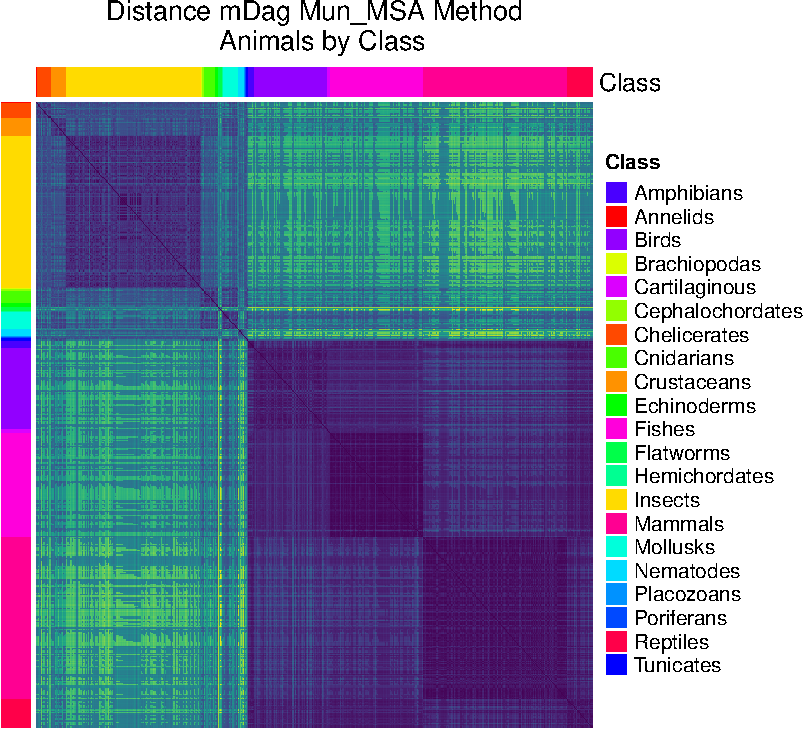
\includegraphics{./data_medag_20230321_long_report_files/figure-pdf/unnamed-chunk-16-1.pdf}

}

\end{figure}

\hypertarget{mds-multidimensional-scaling-1}{%
\section{MDS (Multidimensional
Scaling)}\label{mds-multidimensional-scaling-1}}

\begin{Shaded}
\begin{Highlighting}[]
\DocumentationTok{\#\# Metric multidimensional scaling (mMDS)}
\NormalTok{mds7 }\OtherTok{\textless{}{-}} \FunctionTok{cmdscale}\NormalTok{(}\FunctionTok{sqrt}\NormalTok{(}\DecValTok{1}\SpecialCharTok{{-}}\NormalTok{Sim\_Mun\_MSA\_mDAG}\SpecialCharTok{\^{}}\DecValTok{2}\NormalTok{),}\AttributeTok{k=}\DecValTok{7}\NormalTok{,}\AttributeTok{eig=}\ConstantTok{TRUE}\NormalTok{)}
\CommentTok{\#pairs(mds7$points[,1:4])}
\NormalTok{mds7}\SpecialCharTok{$}\NormalTok{GOF}
\end{Highlighting}
\end{Shaded}

\begin{verbatim}
[1] 0.4464797 0.5474100
\end{verbatim}

\begin{Shaded}
\begin{Highlighting}[]
\NormalTok{mds }\OtherTok{\textless{}{-}}\NormalTok{ mds7}\SpecialCharTok{$}\NormalTok{points }\SpecialCharTok{\%\textgreater{}\%}  \FunctionTok{as\_tibble}\NormalTok{()}
\FunctionTok{colnames}\NormalTok{(mds) }\OtherTok{\textless{}{-}}\FunctionTok{paste0}\NormalTok{(}\StringTok{"Dim."}\NormalTok{,}\DecValTok{1}\SpecialCharTok{:}\FunctionTok{dim}\NormalTok{(mds7}\SpecialCharTok{$}\NormalTok{points)[}\DecValTok{2}\NormalTok{])}

\FunctionTok{library}\NormalTok{(GGally)}

\FunctionTok{ggpairs}\NormalTok{(}\FunctionTok{as\_tibble}\NormalTok{(mds7}\SpecialCharTok{$}\NormalTok{points),}\AttributeTok{columns=}\DecValTok{1}\SpecialCharTok{:}\DecValTok{4}\NormalTok{,}\FunctionTok{aes}\NormalTok{(}\AttributeTok{color=}\NormalTok{meta\_taxo}\SpecialCharTok{$}\NormalTok{Kingdom,}\AttributeTok{alpha=}\FloatTok{0.5}\NormalTok{),}\AttributeTok{upper=}\FunctionTok{list}\NormalTok{(}\AttributeTok{continuous=}\StringTok{"points"}\NormalTok{)) }
\end{Highlighting}
\end{Shaded}

\begin{figure}[H]

{\centering 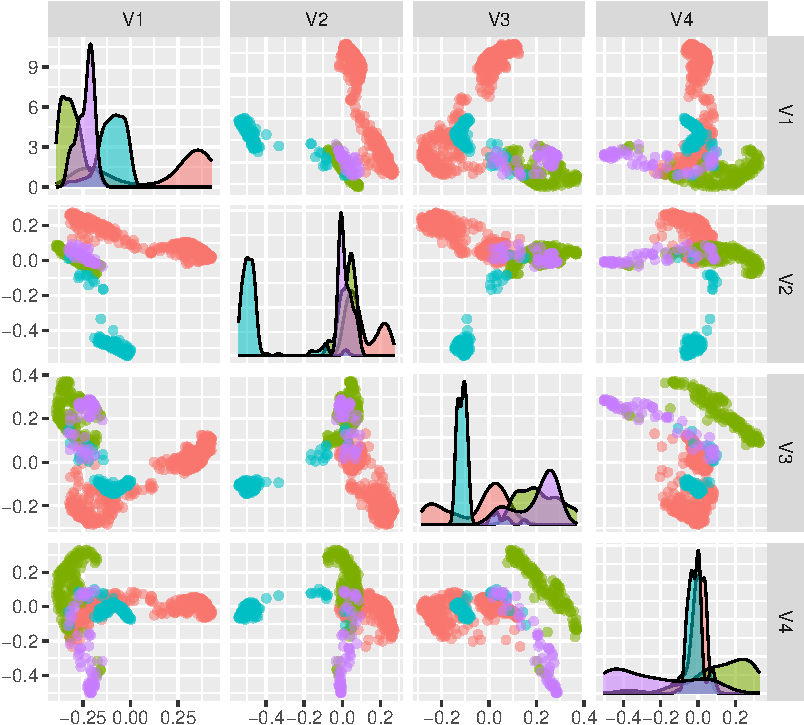
\includegraphics{./data_medag_20230321_long_report_files/figure-pdf/unnamed-chunk-17-1.pdf}

}

\end{figure}

\begin{Shaded}
\begin{Highlighting}[]
\CommentTok{\#cmdscale(D,2,eig=TRUE)$GOF}

\CommentTok{\# Plot MDS}

\CommentTok{\#mds \textless{}{-} mds \%\textgreater{}\%}
 \CommentTok{\# mutate(groups =as.factor(sim0\_meta$Kingdom))}

\NormalTok{mds }\OtherTok{\textless{}{-}}\NormalTok{ mds }\SpecialCharTok{\%\textgreater{}\%}
  \FunctionTok{mutate}\NormalTok{(}\AttributeTok{groups =}\FunctionTok{as.factor}\NormalTok{(meta\_taxo}\SpecialCharTok{$}\NormalTok{Kingdom))}


\CommentTok{\#,text= \textasciitilde{}paste("Age:", groups, \textquotesingle{}\textless{}br\textgreater{}Name:\textquotesingle{})}
\FunctionTok{length}\NormalTok{(}\FunctionTok{unique}\NormalTok{(meta\_taxo}\SpecialCharTok{$}\NormalTok{Phylum))}
\end{Highlighting}
\end{Shaded}

\begin{verbatim}
[1] 33
\end{verbatim}

\begin{Shaded}
\begin{Highlighting}[]
\CommentTok{\#col\_mds=c("purple","green","yellow","coral")}
\NormalTok{col\_mds}\OtherTok{=}\FunctionTok{rainbow}\NormalTok{(}\DecValTok{33}\NormalTok{)}
\CommentTok{\#mcol\_mds=bremer.pal(7,"Greens")}

\NormalTok{fig }\OtherTok{\textless{}{-}} 
\FunctionTok{plot\_ly}\NormalTok{(}
\NormalTok{  mds, }\AttributeTok{x =} \SpecialCharTok{\textasciitilde{}}\NormalTok{Dim}\FloatTok{.1}\NormalTok{, }\AttributeTok{y =} \SpecialCharTok{\textasciitilde{}}\NormalTok{Dim}\FloatTok{.2}\NormalTok{,}
  \AttributeTok{color =} \SpecialCharTok{\textasciitilde{}}\NormalTok{groups, }
  \AttributeTok{colors=}\NormalTok{ col\_mds}
\NormalTok{) }\SpecialCharTok{\%\textgreater{}\%}
  \FunctionTok{layout}\NormalTok{(}
    \AttributeTok{xaxis =} \FunctionTok{list}\NormalTok{(}\AttributeTok{autorange=}\DecValTok{2}\NormalTok{,}
      \AttributeTok{range=}\FunctionTok{c}\NormalTok{(}\SpecialCharTok{{-}}\FloatTok{0.8}\NormalTok{,}\FloatTok{0.8}\NormalTok{)), }\AttributeTok{yaxis =} \FunctionTok{list}\NormalTok{(}\AttributeTok{autorange=}\DecValTok{2}\NormalTok{,}
      \AttributeTok{range=}\FunctionTok{c}\NormalTok{(}\SpecialCharTok{{-}}\FloatTok{0.8}\NormalTok{,}\FloatTok{0.8}\NormalTok{)))}
\CommentTok{\#fig}
\end{Highlighting}
\end{Shaded}

\bookmarksetup{startatroot}

\hypertarget{hierarchical-cluster-1}{%
\chapter{Hierarchical cluster}\label{hierarchical-cluster-1}}

\begin{Shaded}
\begin{Highlighting}[]
\FunctionTok{library}\NormalTok{(dendextend)}
\NormalTok{D}\OtherTok{=}\FunctionTok{as.dist}\NormalTok{(}\FunctionTok{sqrt}\NormalTok{(}\DecValTok{1}\SpecialCharTok{{-}}\NormalTok{Sim\_Mun\_MSA\_mDAG}\SpecialCharTok{\^{}}\DecValTok{2}\NormalTok{))}
\NormalTok{hc}\OtherTok{=}\FunctionTok{hclust}\NormalTok{(}\FunctionTok{as.dist}\NormalTok{(D),}\AttributeTok{method =}\StringTok{"ward.D"}\NormalTok{)}
\FunctionTok{ggplot}\NormalTok{(}\FunctionTok{as.ggdend}\NormalTok{(}\FunctionTok{as.dendrogram}\NormalTok{(hc)))}
\end{Highlighting}
\end{Shaded}

\begin{figure}[H]

{\centering 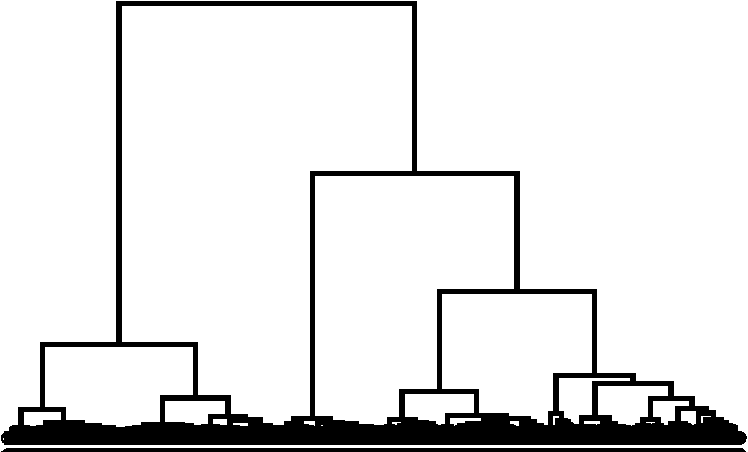
\includegraphics{./data_medag_20230321_long_report_files/figure-pdf/unnamed-chunk-18-1.pdf}

}

\end{figure}

\begin{Shaded}
\begin{Highlighting}[]
\NormalTok{clust4}\OtherTok{=}\FunctionTok{cutree}\NormalTok{(hc,}\DecValTok{4}\NormalTok{)}
\FunctionTok{table}\NormalTok{(clust4,meta\_taxo}\SpecialCharTok{$}\NormalTok{Kingdom)}
\end{Highlighting}
\end{Shaded}

\begin{verbatim}
      
clust4 Animals Fungi Plants Protists
     1     197     0      0        0
     2       7   154     14       56
     3     331     0      0        0
     4       0     0    125        0
\end{verbatim}

\bookmarksetup{startatroot}

\hypertarget{load-data-graphs}{%
\chapter{Load data graphs}\label{load-data-graphs}}

\hypertarget{read-all-graphs-from-a-level-of-the-experiment}{%
\section{Read all graphs from a level of the
experiment}\label{read-all-graphs-from-a-level-of-the-experiment}}

Read all graphs from a level from experiment; for example individuals.
We read only firts (alphabetic) two graph

\begin{Shaded}
\begin{Highlighting}[]
\NormalTok{path\_exp}\OtherTok{=}\StringTok{"data/results\_ff15c187{-}62e7{-}37c2{-}96a7{-}c824f7eab671/data/"}
\NormalTok{list\_names}\OtherTok{=}\FunctionTok{dir}\NormalTok{(}\FunctionTok{paste0}\NormalTok{(path\_exp,}\StringTok{"Individuals/"}\NormalTok{))}
\NormalTok{list\_names}
\end{Highlighting}
\end{Shaded}

\begin{verbatim}
  [1] "0000_RefPw" "aaf"        "aag"        "aalb"       "aali"      
  [6] "aalt"       "aam"        "aamp"       "aang"       "aara"      
 [11] "abe"        "abp"        "abv"        "acan"       "acar"      
 [16] "acep"       "acer"       "achc"       "ache"       "achl"      
 [21] "acoz"       "acs"        "act"        "acun"       "acyg"      
 [26] "adf"        "adl"        "adu"        "aec"        "afm"       
 [31] "afor"       "aful"       "afv"        "afz"        "aga"       
 [36] "agb"        "agen"       "agif"       "ago"        "agrg"      
 [41] "ags"        "ahf"        "aip"        "ajc"        "aje"       
 [46] "ajm"        "aju"        "alab"       "alat"       "alim"      
 [51] "aluc"       "aly"        "ame"        "amer"       "amex"      
 [56] "amil"       "amj"        "aml"        "ang"        "ani"       
 [61] "anu"        "aoce"       "aof"        "aor"        "apan"      
 [66] "api"        "apla"       "aplc"       "apln"       "aprc"      
 [71] "apro"       "apuu"       "aqu"        "arow"       "arut"      
 [76] "asn"        "aste"       "atd"        "aten"       "ath"       
 [81] "atr"        "ats"        "avit"       "bacu"       "bany"      
 [86] "bbel"       "bbif"       "bbig"       "bbis"       "bbo"       
 [91] "bbrx"       "bbub"       "bbuf"       "bcom"       "bcoo"      
 [96] "bdi"        "beq"        "bfo"        "bfu"        "bgar"      
[101] "bgh"        "bgt"        "bhj"        "bim"        "biu"       
[106] "bman"       "bmic"       "bmor"       "bmy"        "bna"       
[111] "bnn"        "bod"        "boe"        "bom"        "bor"       
[116] "bpec"       "bpg"        "bpyo"       "brhi"       "brp"       
[121] "bsc"        "bspl"       "bta"        "btab"       "btax"      
[126] "bter"       "bvan"       "bvg"        "bvk"        "bze"       
[131] "cabi"       "cal"        "cam"        "cang"       "cann"      
[136] "caty"       "caua"       "caur"       "cbai"       "cbr"       
[141] "cbrc"       "ccad"       "ccae"       "ccaj"       "ccal"      
[146] "ccan"       "ccar"       "ccat"       "ccav"       "cci"       
[151] "ccin"       "cclu"       "ccp"        "ccrc"       "ccri"      
[156] "ccw"        "cdk"        "cdu"        "cel"        "cfa"       
[161] "cfel"       "cfj"        "cfo"        "cfr"        "cge"       
[166] "cgi"        "cgib"       "cgig"       "cglo"       "cgob"      
[171] "cgr"        "chig"       "cho"        "chx"        "cic"       
[176] "cide"       "cill"       "cim"        "cimi"       "cin"       
[181] "cins"       "cit"        "cjc"        "cjo"        "clec"      
[186] "clu"        "clud"       "clup"       "clus"       "clv"       
[191] "cmac"       "cmax"       "cme"        "cmk"        "cmo"       
[196] "cmos"       "cmt"        "cmy"        "cnb"        "cne"       
[201] "cng"        "cns"        "cot"        "cpap"       "cpea"      
[206] "cpep"       "cpic"       "cpii"       "cpla"       "cpoc"      
[211] "cpoo"       "cput"       "cpv"        "cpw"        "cqi"       
[216] "cqu"        "crb"        "cre"        "crg"        "csab"      
[221] "csat"       "cscu"       "csec"       "csem"       "cset"      
[226] "csin"       "csl"        "csol"       "csti"       "csv"       
[231] "csyr"       "cten"       "cthr"       "ctig"       "ctp"       
[236] "ctul"       "cuca"       "cud"        "cvf"        "cvg"       
[241] "cvr"        "dam"        "dan"        "daz"        "dci"       
[246] "dcr"        "dct"        "ddi"        "der"        "dfa"       
[251] "dfr"        "dgr"        "dgt"        "dha"        "dhe"       
[256] "dle"        "dme"        "dmk"        "dmn"        "dmo"       
[261] "dne"        "dnm"        "dnv"        "dnx"        "dord"      
[266] "dosa"       "dpa"        "dpe"        "dpl"        "dpo"       
[271] "dpol"       "dpp"        "dpte"       "dpub"       "dpx"       
[276] "dpz"        "dqu"        "dre"        "dro"        "dse"       
[281] "dsi"        "dsm"        "dsp"        "dsq"        "dsr"       
[286] "dsv"        "dvi"        "dwi"        "dya"        "dzi"       
[291] "eaf"        "eai"        "ecad"       "ecb"        "ecra"      
[296] "ecu"        "edi"        "eee"        "efo"        "egl"       
[301] "egr"        "egt"        "egu"        "egz"        "ehe"       
[306] "ehi"        "ehs"        "ehx"        "ein"        "eiv"       
[311] "eju"        "ela"        "elk"        "els"        "ely"       
[316] "epa"        "epz"        "erc"        "ero"        "esn"       
[321] "esp"        "etf"        "etl"        "eus"        "fab"       
[326] "fas"        "fca"        "fcd"        "fch"        "fcy"       
[331] "fex"        "ffu"        "fga"        "fgr"        "fme"       
[336] "foc"        "fox"        "fpg"        "fpu"        "fve"       
[341] "fvr"        "gab"        "gae"        "gaf"        "gas"       
[346] "gat"        "gcl"        "gfr"        "gga"        "ggn"       
[351] "ggo"        "ghi"        "gja"        "gla"        "glz"       
[356] "gmu"        "gmx"        "gra"        "gsj"        "gsl"       
[361] "gste"       "gtr"        "gtt"        "gvr"        "hai"       
[366] "hald"       "hame"       "han"        "haw"        "hazt"      
[371] "hbr"        "hcg"        "hcq"        "hgl"        "hhal"      
[376] "hhip"       "hhv"        "hir"        "his"        "hle"       
[381] "hmg"        "hmh"        "hrf"        "hrj"        "hro"       
[386] "hsa"        "hsp"        "hst"        "hze"        "ini"       
[391] "ipu"        "isc"        "itr"        "jcu"        "jre"       
[396] "kaf"        "kla"        "kmr"        "kmx"        "kng"       
[401] "lak"        "lang"       "lav"        "lbc"        "lbd"       
[406] "lbz"        "lcat"       "lcf"        "lcm"        "lco"       
[411] "lcq"        "ldc"        "ldi"        "ldo"        "lel"       
[416] "lgi"        "lht"        "lhu"        "lif"        "lja"       
[421] "llv"        "lma"        "lmi"        "loa"        "loc"       
[426] "lpan"       "lper"       "lpol"       "lruf"       "lsm"       
[431] "lsq"        "lsr"        "lsv"        "lth"        "lve"       
[436] "lww"        "maj"        "malb"       "mamb"       "masi"      
[441] "maua"       "maw"        "mbe"        "mbr"        "mcaf"      
[446] "mcal"       "mcc"        "mcep"       "mcf"        "mcha"      
[451] "mcoc"       "mde"        "mdl"        "mdm"        "mdo"       
[456] "mesc"       "mfot"       "mgen"       "mgl"        "mgp"       
[461] "mgr"        "minc"       "ming"       "mis"        "mjv"       
[466] "mleu"       "mlf"        "mlr"        "mlx"        "mmer"      
[471] "mmf"        "mmu"        "mmur"       "mmyo"       "mna"       
[476] "mnb"        "mng"        "mni"        "mnt"        "more"      
[481] "morg"       "mpah"       "mpha"       "mpp"        "mpr"       
[486] "mpuf"       "mrr"        "mrt"        "mrv"        "msam"      
[491] "msex"       "msym"       "mthb"       "mtm"        "mtr"       
[496] "mui"        "mun"        "mus"        "myb"        "myd"       
[501] "myi"        "mze"        "nai"        "nasi"       "nau"       
[506] "ncar"       "ncc"        "nce"        "ncol"       "ncr"       
[511] "ncs"        "ndi"        "nfi"        "nfu"        "ngd"       
[516] "ngi"        "ngr"        "nhe"        "niq"        "nle"       
[521] "nlu"        "nmea"       "nmel"       "nni"        "nnt"       
[526] "nnu"        "npa"        "npd"        "npr"        "npt"       
[531] "nsu"        "nsy"        "nta"        "nte"        "nto"       
[536] "nve"        "nvi"        "nvl"        "nvs"        "nwh"       
[541] "oaa"        "oas"        "oau"        "obb"        "obi"       
[546] "obo"        "obr"        "ocu"        "oda"        "oeu"       
[551] "ofu"        "oga"        "ogl"        "ogo"        "oha"       
[556] "ola"        "olu"        "oml"        "omy"        "one"       
[561] "onl"        "oor"        "opa"        "opi"        "oro"       
[566] "osa"        "osn"        "ota"        "otc"        "otu"       
[571] "otw"        "ovi"        "padl"       "pale"       "palz"      
[576] "pan"        "panu"       "pavi"       "pbar"       "pbe"       
[581] "pbg"        "pbi"        "pbl"        "pbn"        "pbx"       
[586] "pcad"       "pcan"       "pcao"       "pcb"        "pcf"       
[591] "pchn"       "pcla"       "pco"        "pcoc"       "pcoo"      
[596] "pcoq"       "pcri"       "pcs"        "pcub"       "pcw"       
[601] "pcy"        "pda"        "pdam"       "pdic"       "pdp"       
[606] "pdul"       "peq"        "peu"        "pfa"        "pfd"       
[611] "pfh"        "pfj"        "pflv"       "pfor"       "pfp"       
[616] "pfuc"       "pfy"        "pgab"       "pgc"        "pgig"      
[621] "pgr"        "pgu"        "pgut"       "pguu"       "phai"      
[626] "phas"       "phi"        "phu"        "phyp"       "pic"       
[631] "pif"        "pja"        "pki"        "pkl"        "pkn"       
[636] "pkz"        "plai"       "plep"       "plet"       "pleu"      
[641] "plj"        "plop"       "pmac"       "pmaj"       "pmax"      
[646] "pmei"       "pmoa"       "pmoo"       "pmua"       "pmum"      
[651] "pmur"       "pnap"       "pno"        "pon"        "pop"       
[656] "pov"        "ppa"        "ppad"       "ppei"       "pper"      
[661] "ppl"        "ppoi"       "ppot"       "ppp"        "pprm"      
[666] "pps"        "ppug"       "ppyr"       "prap"       "prei"      
[671] "pret"       "prob"       "pruf"       "psat"       "psco"      
[676] "psex"       "psiu"       "psoj"       "psom"       "pspa"      
[681] "psq"        "pss"        "pte"        "pteh"       "ptep"      
[686] "ptg"        "pti"        "ptkz"       "ptm"        "ptr"       
[691] "ptru"       "puc"        "pvir"       "pvm"        "pvp"       
[696] "pvt"        "pvu"        "pvv"        "pvx"        "pvy"       
[701] "pxb"        "pxu"        "pxy"        "pyo"        "pyu"       
[706] "qlo"        "qsu"        "ray"        "rbb"        "rcn"       
[711] "rcu"        "rfq"        "rmd"        "rmp"        "rno"       
[716] "rro"        "rsan"       "rsz"        "rtem"       "rtp"       
[721] "rze"        "salp"       "sanh"       "sapo"       "sara"      
[726] "sasa"       "sbi"        "sbq"        "scac"       "scam"      
[731] "scan"       "sce"        "schu"       "sclv"       "scm"       
[736] "sdm"        "sdu"        "seub"       "sfm"        "sgh"       
[741] "sgre"       "shab"       "shon"       "shr"        "shs"       
[746] "shx"        "sind"       "sita"       "sko"        "sla"       
[751] "slal"       "slb"        "sliu"       "sluc"       "slud"      
[756] "sly"        "smeo"       "smin"       "smm"        "smo"       
[761] "smp"        "snh"        "soc"        "soe"        "sot"       
[766] "soy"        "spaa"       "spao"       "spar"       "spen"      
[771] "spis"       "spo"        "spu"        "sre"        "srx"       
[776] "ssc"        "ssck"       "sscv"       "ssen"       "ssl"       
[781] "sspl"       "sstn"       "stow"       "stru"       "sund"      
[786] "svg"        "svs"        "tad"        "taes"       "tala"      
[791] "tan"        "tasa"       "tbg"        "tbl"        "tbr"       
[796] "tca"        "tcc"        "tcr"        "tdc"        "tdl"       
[801] "teo"        "tet"        "tfd"        "tfn"        "tgb"       
[806] "tge"        "tgo"        "tgt"        "tgu"        "thj"       
[811] "tmf"        "tml"        "tmn"        "tms"        "tmu"       
[816] "tng"        "tnl"        "tod"        "tot"        "tpai"      
[821] "tpal"       "tpf"        "tpra"       "tpre"       "tps"       
[826] "tpv"        "tre"        "trg"        "trr"        "tru"       
[831] "tsp"        "tsr"        "tss"        "tst"        "ttt"       
[836] "tua"        "tup"        "tut"        "tva"        "tve"       
[841] "tvs"        "twl"        "uah"        "uar"        "uma"       
[846] "umr"        "ure"        "val"        "var"        "vcn"       
[851] "vda"        "vde"        "vem"        "vja"        "vko"       
[856] "vlg"        "vpc"        "vpo"        "vps"        "vra"       
[861] "vri"        "vun"        "vvi"        "vvp"        "wic"       
[866] "wse"        "xco"        "xen"        "xgl"        "xhe"       
[871] "xla"        "xma"        "xtr"        "yli"        "zab"       
[876] "zca"        "zce"        "zju"        "zma"        "zmk"       
[881] "zne"        "zof"        "zro"        "ztr"        "zvi"       
\end{verbatim}

\begin{Shaded}
\begin{Highlighting}[]
\NormalTok{list\_names}\OtherTok{=}\NormalTok{ list\_names[}\SpecialCharTok{{-}}\DecValTok{1}\NormalTok{] }\CommentTok{\# filter 0000\_RefPw}
\FunctionTok{length}\NormalTok{(list\_names)}
\end{Highlighting}
\end{Shaded}

\begin{verbatim}
[1] 884
\end{verbatim}

\begin{Shaded}
\begin{Highlighting}[]
\NormalTok{k}\OtherTok{=}\FunctionTok{length}\NormalTok{(list\_names)}
\NormalTok{list\_names}\OtherTok{=}\NormalTok{ list\_names[}\DecValTok{1}\SpecialCharTok{:}\NormalTok{k] }\CommentTok{\# select ONLY 5 individuals}
\NormalTok{list\_names}
\end{Highlighting}
\end{Shaded}

\begin{verbatim}
  [1] "aaf"  "aag"  "aalb" "aali" "aalt" "aam"  "aamp" "aang" "aara" "abe" 
 [11] "abp"  "abv"  "acan" "acar" "acep" "acer" "achc" "ache" "achl" "acoz"
 [21] "acs"  "act"  "acun" "acyg" "adf"  "adl"  "adu"  "aec"  "afm"  "afor"
 [31] "aful" "afv"  "afz"  "aga"  "agb"  "agen" "agif" "ago"  "agrg" "ags" 
 [41] "ahf"  "aip"  "ajc"  "aje"  "ajm"  "aju"  "alab" "alat" "alim" "aluc"
 [51] "aly"  "ame"  "amer" "amex" "amil" "amj"  "aml"  "ang"  "ani"  "anu" 
 [61] "aoce" "aof"  "aor"  "apan" "api"  "apla" "aplc" "apln" "aprc" "apro"
 [71] "apuu" "aqu"  "arow" "arut" "asn"  "aste" "atd"  "aten" "ath"  "atr" 
 [81] "ats"  "avit" "bacu" "bany" "bbel" "bbif" "bbig" "bbis" "bbo"  "bbrx"
 [91] "bbub" "bbuf" "bcom" "bcoo" "bdi"  "beq"  "bfo"  "bfu"  "bgar" "bgh" 
[101] "bgt"  "bhj"  "bim"  "biu"  "bman" "bmic" "bmor" "bmy"  "bna"  "bnn" 
[111] "bod"  "boe"  "bom"  "bor"  "bpec" "bpg"  "bpyo" "brhi" "brp"  "bsc" 
[121] "bspl" "bta"  "btab" "btax" "bter" "bvan" "bvg"  "bvk"  "bze"  "cabi"
[131] "cal"  "cam"  "cang" "cann" "caty" "caua" "caur" "cbai" "cbr"  "cbrc"
[141] "ccad" "ccae" "ccaj" "ccal" "ccan" "ccar" "ccat" "ccav" "cci"  "ccin"
[151] "cclu" "ccp"  "ccrc" "ccri" "ccw"  "cdk"  "cdu"  "cel"  "cfa"  "cfel"
[161] "cfj"  "cfo"  "cfr"  "cge"  "cgi"  "cgib" "cgig" "cglo" "cgob" "cgr" 
[171] "chig" "cho"  "chx"  "cic"  "cide" "cill" "cim"  "cimi" "cin"  "cins"
[181] "cit"  "cjc"  "cjo"  "clec" "clu"  "clud" "clup" "clus" "clv"  "cmac"
[191] "cmax" "cme"  "cmk"  "cmo"  "cmos" "cmt"  "cmy"  "cnb"  "cne"  "cng" 
[201] "cns"  "cot"  "cpap" "cpea" "cpep" "cpic" "cpii" "cpla" "cpoc" "cpoo"
[211] "cput" "cpv"  "cpw"  "cqi"  "cqu"  "crb"  "cre"  "crg"  "csab" "csat"
[221] "cscu" "csec" "csem" "cset" "csin" "csl"  "csol" "csti" "csv"  "csyr"
[231] "cten" "cthr" "ctig" "ctp"  "ctul" "cuca" "cud"  "cvf"  "cvg"  "cvr" 
[241] "dam"  "dan"  "daz"  "dci"  "dcr"  "dct"  "ddi"  "der"  "dfa"  "dfr" 
[251] "dgr"  "dgt"  "dha"  "dhe"  "dle"  "dme"  "dmk"  "dmn"  "dmo"  "dne" 
[261] "dnm"  "dnv"  "dnx"  "dord" "dosa" "dpa"  "dpe"  "dpl"  "dpo"  "dpol"
[271] "dpp"  "dpte" "dpub" "dpx"  "dpz"  "dqu"  "dre"  "dro"  "dse"  "dsi" 
[281] "dsm"  "dsp"  "dsq"  "dsr"  "dsv"  "dvi"  "dwi"  "dya"  "dzi"  "eaf" 
[291] "eai"  "ecad" "ecb"  "ecra" "ecu"  "edi"  "eee"  "efo"  "egl"  "egr" 
[301] "egt"  "egu"  "egz"  "ehe"  "ehi"  "ehs"  "ehx"  "ein"  "eiv"  "eju" 
[311] "ela"  "elk"  "els"  "ely"  "epa"  "epz"  "erc"  "ero"  "esn"  "esp" 
[321] "etf"  "etl"  "eus"  "fab"  "fas"  "fca"  "fcd"  "fch"  "fcy"  "fex" 
[331] "ffu"  "fga"  "fgr"  "fme"  "foc"  "fox"  "fpg"  "fpu"  "fve"  "fvr" 
[341] "gab"  "gae"  "gaf"  "gas"  "gat"  "gcl"  "gfr"  "gga"  "ggn"  "ggo" 
[351] "ghi"  "gja"  "gla"  "glz"  "gmu"  "gmx"  "gra"  "gsj"  "gsl"  "gste"
[361] "gtr"  "gtt"  "gvr"  "hai"  "hald" "hame" "han"  "haw"  "hazt" "hbr" 
[371] "hcg"  "hcq"  "hgl"  "hhal" "hhip" "hhv"  "hir"  "his"  "hle"  "hmg" 
[381] "hmh"  "hrf"  "hrj"  "hro"  "hsa"  "hsp"  "hst"  "hze"  "ini"  "ipu" 
[391] "isc"  "itr"  "jcu"  "jre"  "kaf"  "kla"  "kmr"  "kmx"  "kng"  "lak" 
[401] "lang" "lav"  "lbc"  "lbd"  "lbz"  "lcat" "lcf"  "lcm"  "lco"  "lcq" 
[411] "ldc"  "ldi"  "ldo"  "lel"  "lgi"  "lht"  "lhu"  "lif"  "lja"  "llv" 
[421] "lma"  "lmi"  "loa"  "loc"  "lpan" "lper" "lpol" "lruf" "lsm"  "lsq" 
[431] "lsr"  "lsv"  "lth"  "lve"  "lww"  "maj"  "malb" "mamb" "masi" "maua"
[441] "maw"  "mbe"  "mbr"  "mcaf" "mcal" "mcc"  "mcep" "mcf"  "mcha" "mcoc"
[451] "mde"  "mdl"  "mdm"  "mdo"  "mesc" "mfot" "mgen" "mgl"  "mgp"  "mgr" 
[461] "minc" "ming" "mis"  "mjv"  "mleu" "mlf"  "mlr"  "mlx"  "mmer" "mmf" 
[471] "mmu"  "mmur" "mmyo" "mna"  "mnb"  "mng"  "mni"  "mnt"  "more" "morg"
[481] "mpah" "mpha" "mpp"  "mpr"  "mpuf" "mrr"  "mrt"  "mrv"  "msam" "msex"
[491] "msym" "mthb" "mtm"  "mtr"  "mui"  "mun"  "mus"  "myb"  "myd"  "myi" 
[501] "mze"  "nai"  "nasi" "nau"  "ncar" "ncc"  "nce"  "ncol" "ncr"  "ncs" 
[511] "ndi"  "nfi"  "nfu"  "ngd"  "ngi"  "ngr"  "nhe"  "niq"  "nle"  "nlu" 
[521] "nmea" "nmel" "nni"  "nnt"  "nnu"  "npa"  "npd"  "npr"  "npt"  "nsu" 
[531] "nsy"  "nta"  "nte"  "nto"  "nve"  "nvi"  "nvl"  "nvs"  "nwh"  "oaa" 
[541] "oas"  "oau"  "obb"  "obi"  "obo"  "obr"  "ocu"  "oda"  "oeu"  "ofu" 
[551] "oga"  "ogl"  "ogo"  "oha"  "ola"  "olu"  "oml"  "omy"  "one"  "onl" 
[561] "oor"  "opa"  "opi"  "oro"  "osa"  "osn"  "ota"  "otc"  "otu"  "otw" 
[571] "ovi"  "padl" "pale" "palz" "pan"  "panu" "pavi" "pbar" "pbe"  "pbg" 
[581] "pbi"  "pbl"  "pbn"  "pbx"  "pcad" "pcan" "pcao" "pcb"  "pcf"  "pchn"
[591] "pcla" "pco"  "pcoc" "pcoo" "pcoq" "pcri" "pcs"  "pcub" "pcw"  "pcy" 
[601] "pda"  "pdam" "pdic" "pdp"  "pdul" "peq"  "peu"  "pfa"  "pfd"  "pfh" 
[611] "pfj"  "pflv" "pfor" "pfp"  "pfuc" "pfy"  "pgab" "pgc"  "pgig" "pgr" 
[621] "pgu"  "pgut" "pguu" "phai" "phas" "phi"  "phu"  "phyp" "pic"  "pif" 
[631] "pja"  "pki"  "pkl"  "pkn"  "pkz"  "plai" "plep" "plet" "pleu" "plj" 
[641] "plop" "pmac" "pmaj" "pmax" "pmei" "pmoa" "pmoo" "pmua" "pmum" "pmur"
[651] "pnap" "pno"  "pon"  "pop"  "pov"  "ppa"  "ppad" "ppei" "pper" "ppl" 
[661] "ppoi" "ppot" "ppp"  "pprm" "pps"  "ppug" "ppyr" "prap" "prei" "pret"
[671] "prob" "pruf" "psat" "psco" "psex" "psiu" "psoj" "psom" "pspa" "psq" 
[681] "pss"  "pte"  "pteh" "ptep" "ptg"  "pti"  "ptkz" "ptm"  "ptr"  "ptru"
[691] "puc"  "pvir" "pvm"  "pvp"  "pvt"  "pvu"  "pvv"  "pvx"  "pvy"  "pxb" 
[701] "pxu"  "pxy"  "pyo"  "pyu"  "qlo"  "qsu"  "ray"  "rbb"  "rcn"  "rcu" 
[711] "rfq"  "rmd"  "rmp"  "rno"  "rro"  "rsan" "rsz"  "rtem" "rtp"  "rze" 
[721] "salp" "sanh" "sapo" "sara" "sasa" "sbi"  "sbq"  "scac" "scam" "scan"
[731] "sce"  "schu" "sclv" "scm"  "sdm"  "sdu"  "seub" "sfm"  "sgh"  "sgre"
[741] "shab" "shon" "shr"  "shs"  "shx"  "sind" "sita" "sko"  "sla"  "slal"
[751] "slb"  "sliu" "sluc" "slud" "sly"  "smeo" "smin" "smm"  "smo"  "smp" 
[761] "snh"  "soc"  "soe"  "sot"  "soy"  "spaa" "spao" "spar" "spen" "spis"
[771] "spo"  "spu"  "sre"  "srx"  "ssc"  "ssck" "sscv" "ssen" "ssl"  "sspl"
[781] "sstn" "stow" "stru" "sund" "svg"  "svs"  "tad"  "taes" "tala" "tan" 
[791] "tasa" "tbg"  "tbl"  "tbr"  "tca"  "tcc"  "tcr"  "tdc"  "tdl"  "teo" 
[801] "tet"  "tfd"  "tfn"  "tgb"  "tge"  "tgo"  "tgt"  "tgu"  "thj"  "tmf" 
[811] "tml"  "tmn"  "tms"  "tmu"  "tng"  "tnl"  "tod"  "tot"  "tpai" "tpal"
[821] "tpf"  "tpra" "tpre" "tps"  "tpv"  "tre"  "trg"  "trr"  "tru"  "tsp" 
[831] "tsr"  "tss"  "tst"  "ttt"  "tua"  "tup"  "tut"  "tva"  "tve"  "tvs" 
[841] "twl"  "uah"  "uar"  "uma"  "umr"  "ure"  "val"  "var"  "vcn"  "vda" 
[851] "vde"  "vem"  "vja"  "vko"  "vlg"  "vpc"  "vpo"  "vps"  "vra"  "vri" 
[861] "vun"  "vvi"  "vvp"  "wic"  "wse"  "xco"  "xen"  "xgl"  "xhe"  "xla" 
[871] "xma"  "xtr"  "yli"  "zab"  "zca"  "zce"  "zju"  "zma"  "zmk"  "zne" 
[881] "zof"  "zro"  "ztr"  "zvi" 
\end{verbatim}

\begin{Shaded}
\begin{Highlighting}[]
\FunctionTok{dir}\NormalTok{(}\FunctionTok{paste0}\NormalTok{(}\StringTok{"Individuals/"}\NormalTok{,list\_names[}\DecValTok{1}\NormalTok{],}\StringTok{"/"}\NormalTok{))}
\end{Highlighting}
\end{Shaded}

\begin{verbatim}
character(0)
\end{verbatim}

\begin{Shaded}
\begin{Highlighting}[]
\FunctionTok{library}\NormalTok{(igraph)}
\end{Highlighting}
\end{Shaded}

\begin{verbatim}

Attaching package: 'igraph'
\end{verbatim}

\begin{verbatim}
The following objects are masked from 'package:stats':

    decompose, spectrum
\end{verbatim}

\begin{verbatim}
The following object is masked from 'package:base':

    union
\end{verbatim}

\begin{Shaded}
\begin{Highlighting}[]
\NormalTok{graphs\_list}\OtherTok{=}\FunctionTok{paste0}\NormalTok{(path\_exp,}\StringTok{"Individuals/"}\NormalTok{,list\_names,}\StringTok{"/"}\NormalTok{,list\_names,}\StringTok{"\_MDAG.graphml"}\NormalTok{)}
\NormalTok{g\_MDAG\_list}\OtherTok{=}
  \FunctionTok{lapply}\NormalTok{(graphs\_list,}\AttributeTok{FUN=}\ControlFlowTok{function}\NormalTok{(x) }\FunctionTok{read.graph}\NormalTok{(}\AttributeTok{file=}\NormalTok{x,}
                    \AttributeTok{format=}\StringTok{"graphml"}\NormalTok{))}
\FunctionTok{names}\NormalTok{(g\_MDAG\_list)}\OtherTok{=}\NormalTok{list\_names}
\FunctionTok{summary}\NormalTok{(g\_MDAG\_list[[}\DecValTok{1}\NormalTok{]])}
\end{Highlighting}
\end{Shaded}

\begin{verbatim}
IGRAPH c3835f5 D--- 534 477 -- 
+ attr: color (v/c), label (v/c), id (v/c), id (e/c)
\end{verbatim}

\begin{Shaded}
\begin{Highlighting}[]
\FunctionTok{head}\NormalTok{(}\FunctionTok{as\_long\_data\_frame}\NormalTok{(g\_MDAG\_list[[}\DecValTok{1}\NormalTok{]]))}
\end{Highlighting}
\end{Shaded}

\begin{verbatim}
  from to              id from_color                   from_label from_id
1    2  1       2431x1532     yellow    2431\\nR07762\\n2.3.1.179    2431
2    3  2    0.0.237x2431       gray                MBB\\n0.0.237 0.0.237
3    4  3 0.0.752x0.0.237     yellow 0.0.752\\nR04968\\n2.3.1.179 0.0.752
4    5  4 0.0.238x0.0.752       gray                MBB\\n0.0.238 0.0.238
5    6  5 0.0.753x0.0.238     yellow 0.0.753\\nR04726\\n2.3.1.179 0.0.753
6    7  6 0.0.239x0.0.753       gray                MBB\\n0.0.239 0.0.239
  to_color                     to_label   to_id
1     gray                   MBB\\n1532    1532
2   yellow    2431\\nR07762\\n2.3.1.179    2431
3     gray                MBB\\n0.0.237 0.0.237
4   yellow 0.0.752\\nR04968\\n2.3.1.179 0.0.752
5     gray                MBB\\n0.0.238 0.0.238
6   yellow 0.0.753\\nR04726\\n2.3.1.179 0.0.753
\end{verbatim}

\textbf{Graph Kernels package}

\href{https://academic.oup.com/bioinformatics/article/34/3/530/4209994?login=true}{graphkernels:
R and Python packages for graph comparison} statGraph'
\href{https://journals.plos.org/plosone/article?id=10.1371/journal.pone.0049949}{Discriminating
Different Classes of Biological Networks by Analyzing the Graphs Spectra
Distribution}

\begin{Shaded}
\begin{Highlighting}[]
\FunctionTok{plot.igraph}\NormalTok{(g\_MDAG\_list[[}\DecValTok{1}\NormalTok{]],}\AttributeTok{layout=}\NormalTok{layout\_as\_tree,}
            \AttributeTok{label=}\ConstantTok{NA}\NormalTok{,}\AttributeTok{label.cex=}\DecValTok{0}\NormalTok{)}
\end{Highlighting}
\end{Shaded}

\begin{figure}[H]

{\centering 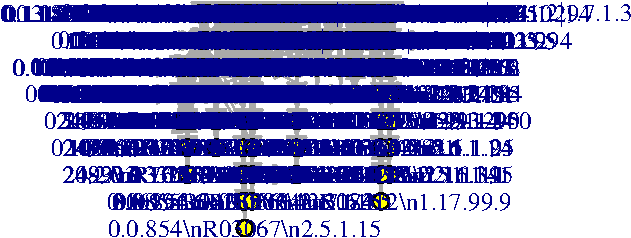
\includegraphics{./kernel_1_files/figure-pdf/unnamed-chunk-2-1.pdf}

}

\end{figure}

\begin{Shaded}
\begin{Highlighting}[]
\NormalTok{knitr}\SpecialCharTok{::}\FunctionTok{include\_graphics}\NormalTok{(}
  \FunctionTok{paste0}\NormalTok{(path\_exp,}\StringTok{"Individuals/cang/cang\_mDAG.svg"}\NormalTok{))}
\end{Highlighting}
\end{Shaded}

\begin{figure}[H]

{\centering 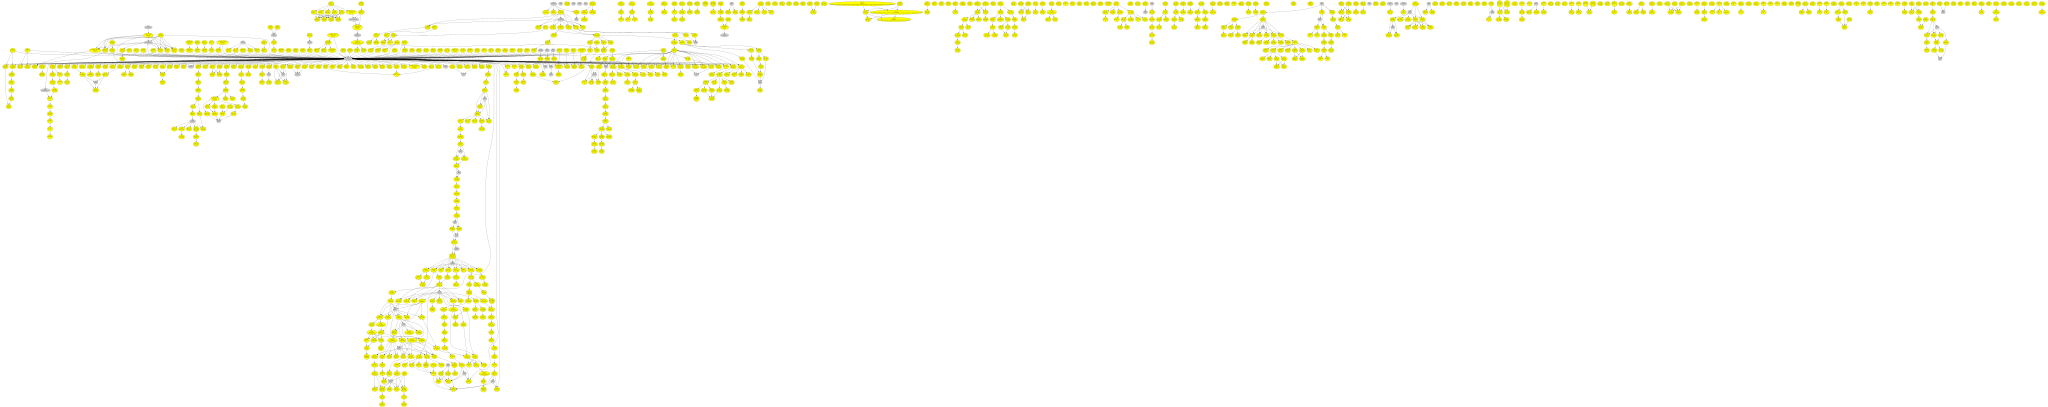
\includegraphics{./data/results_ff15c187-62e7-37c2-96a7-c824f7eab671/data/Individuals/cang/cang_mDAG.svg}

}

\end{figure}

\begin{Shaded}
\begin{Highlighting}[]
\NormalTok{knitr}\SpecialCharTok{::}\FunctionTok{include\_graphics}\NormalTok{(}\FunctionTok{paste0}\NormalTok{(path\_exp,}\StringTok{"Individuals/cang/cang\_mDAG\_essential.svg"}\NormalTok{))}
\end{Highlighting}
\end{Shaded}

\begin{figure}[H]

{\centering 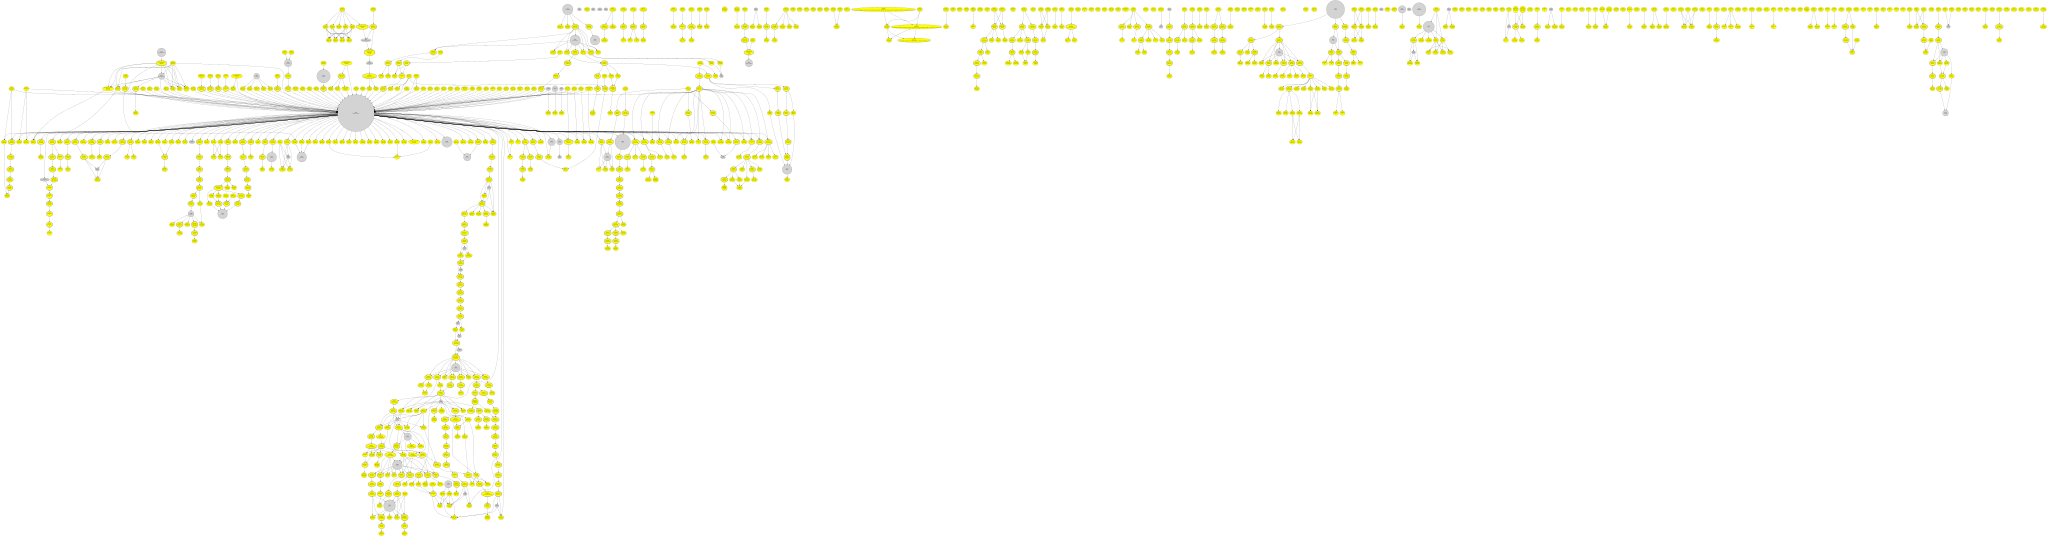
\includegraphics{./data/results_ff15c187-62e7-37c2-96a7-c824f7eab671/data/Individuals/cang/cang_mDAG_essential.svg}

}

\end{figure}

\begin{Shaded}
\begin{Highlighting}[]
\NormalTok{knitr}\SpecialCharTok{::}\FunctionTok{include\_graphics}\NormalTok{(}
  \FunctionTok{paste0}\NormalTok{(path\_exp,}\StringTok{"Individuals/cang/cang\_RC.svg"}\NormalTok{))}
\end{Highlighting}
\end{Shaded}

\begin{figure}[H]

{\centering \includegraphics{./data/results_ff15c187-62e7-37c2-96a7-c824f7eab671/data/Individuals/cang/cang_RC.svg}

}

\end{figure}

\begin{verbatim}
library(DOT)
dot(paste0(path_exp,"Individuals/aag/aag_mDAG2.dot"),
    return="svg")
\end{verbatim}

\bookmarksetup{startatroot}

\hypertarget{references}{%
\chapter*{References}\label{references}}
\addcontentsline{toc}{chapter}{References}

\markboth{References}{References}

\hypertarget{refs}{}
\begin{CSLReferences}{0}{0}
\end{CSLReferences}



\end{document}
